% Importamos el preámbulo con la configuración del documento
% Definición de la clase del documento
\documentclass[a4paper, 11pt]{book} % A4 paper and 11pt font size

% Entrada y salida de texto
\usepackage[T1]{fontenc}
\usepackage[utf8]{inputenc}
\usepackage[sfdefault]{roboto} % Option 'sfdefault' only if the base font of the document is to be sans serif

% Idioma
\usepackage[spanish, es-tabla]{babel} % Selecciona el español y el uso de la palabra "tabla" en lugar de "cuadro"

% Información reutilizable
\newcommand{\asunto}{Trabajo de Fin de Grado}
\newcommand{\titulo}{Juego de tablero aumentado utilizando ARCore}
\newcommand{\tituloEng}{Augmented board game using ARCore}
\newcommand{\subtitulo}{Desarrollo de un juego de mesa aumentado mediante uso de tecnologías de realidad aumentada}
\newcommand{\subtituloEng}{Development of augmented board game using augmented reality technologies}
\newcommand{\grado}{Grado en Ingeniería Informática}
\newcommand{\autor}{Miguel Ángel Torres López}
\newcommand{\email}{matl1995@correo.ugr.es}
\newcommand{\tutor}{Francisco Luis Gutiérrez Vela}
\newcommand{\escuela}{Escuela Técnica Superior de Ingenierías Informática y de Telecomunicación}
\newcommand{\departamento}{Departamento de Lenguajes y Sistemas Informáticos}
\newcommand{\universidad}{Universidad de Granada}
\newcommand{\ciudad}{Granada}
\providecommand{\keywords}{ARCore, Unity, Android, juegos de mesa}
\providecommand{\keywordsEng}{ARCore, Unity, Android, board games}

% Otros paquetes importantes para el proyecto
\usepackage[hyphens]{url}
\usepackage{eurosym}
\usepackage{graphicx}
\usepackage{colortbl}
\usepackage{fancyhdr}
\usepackage{pdfpages}
\usepackage{longtable}
\usepackage[hidelinks]{hyperref}
\usepackage{placeins}
\usepackage{verbatim}

\setcounter{tocdepth}{4}
\setcounter{secnumdepth}{4}

% Añade aquí las carpetas de imágenes para que el compilador las pueda analizar
\graphicspath{{../images/}{../screenshots/}{../images/applications/}{../images/integration/}{../images/techniques/}{../images/mockups/}{../images/headmounted/}{../images/tangibleinterfaces/}{../images/estudiomercado1/}{../images/estudiomercado2/}{../images/metodologias/}{../images/desarrollo/}{../images/entrega2/}}

% Información del archivo
\hypersetup{
  pdfauthor = {\autor\ (\email)},
  pdftitle = {\titulo: \subtitulo},
  pdfsubject = {\asunto},
  pdfkeywords = {\keywords},
  pdfcreator = {LaTeX, con la distribución TeX Live},
  pdfproducer = {pdflatex}
}

% Modificación para que las páginas en blanco no tengan cabecera
\makeatletter
\def\clearpage{
  \ifvmode
    \ifnum \@dbltopnum = \m@ne
      \ifdim \pagetotal < \topskip
        \hbox{}
      \fi
    \fi
  \fi
  \newpage
  \thispagestyle{empty}
  \write\m@ne{}
  \vbox{}
  \penalty -\@Mi
}
\makeatother

% Definición del estilo de las cabeceras
\pagestyle{fancy}
\fancyhf{}
\fancyhead[LO]{\leftmark}
\fancyhead[RE]{\rightmark}
\fancyhead[RO,LE]{\textbf{\thepage}}
\setlength{\headheight}{1.5\headheight}

% Definición de colores
\definecolor{Gray}{gray}{0.9}

% Redefinición de comandos
\renewcommand{\chaptermark}[1]{\markboth{\textbf{#1}}{}}
\renewcommand{\sectionmark}[1]{\markright{\textbf{\thesection. #1}}{}}
% \renewcommand{\lstlistingname}{Fragmento de código}
% \renewcommand{\lstlistlistingname}{Índice de fragmentos de código}

% Creación de comandos
% \newcommand{\HRule}{\rule{\linewidth}{0.5mm}}
% \newcommand{\bigrule}{\titlerule[0.5mm]}

% Ajuste para minimizar el fragmentado de listados
% \lstnewenvironment{listing}[1][]
%   {\lstset{#1}\pagebreak[0]}{\pagebreak[0]}


\begin{document}

% Portada del documento
\begin{titlepage}

\newlength{\centeroffset}
\setlength{\centeroffset}{-0.5\oddsidemargin}
\addtolength{\centeroffset}{0.5\evensidemargin}

\noindent\hspace*{\centeroffset}

\begin{minipage}{\textwidth}

\centering


\includegraphics[width=0.9\textwidth]{logo_ugr}\\[1.4cm]

\textsc{\Large\asunto\\[0.2cm]}
\textsc{\grado}\\[1cm]

{\Huge\bfseries\titulo\\}
\noindent\rule[-1ex]{\textwidth}{3pt}\\[3.5ex]
{\large\bfseries\subtitulo}

\end{minipage}

\vspace{1.5cm}
\noindent\hspace*{\centeroffset}

\begin{minipage}{\textwidth}

\centering

\textbf{Autor}\\{\autor}\\[2.5ex]
\textbf{Tutor}\\{\tutor}\\[1.5cm]


\includegraphics[width=0.3\textwidth]{logo_etsiit}\\[0.1cm]

\textsc{\escuela}\\
\textsc{---}\\
\ciudad, \today\\

\end{minipage}

\end{titlepage}


% Prefacio del documento
\cleardoublepage
\thispagestyle{empty}

\begin{center}
{\LARGE\bfseries\titulo: \subtitulo}\\
\end{center}
\begin{center}
\autor
\end{center}

\bigskip
\noindent{\textbf{Palabras clave}: \textit{\keywords}\\

\section*{Resumen}
Este documento expone mi trabajo de fin de grado, y los contenidos asociados al mismo.\\

Este proyecto se va a centrar en la planificación y desarrollo de un juego de mesa, que mediante las tecnologías de realidad aumentada, mas concretamente ARCore, aportará un nuevo enfoque sobre los juegos de esta temática, aprovechando las singulares características que la realidad aumentada ofrece.\\

El objetivo principal del juego es explorar que ventajas puede aportar la realidad aumentada a los juegos en dispositivos móviles, y mas específicamente a los juegos de mesa en dispositivos móviles.\\

El proyecto explorará también la integración de diferentes formas de interacción en juegos, permitiendo funcionalidades que se tendrán que llevar a cabo mediante interacción con elementos físicos, y otras funcionalidades que se desarrollarán con interacción únicamente con el dispositivo móvil.\\

\cleardoublepage
\thispagestyle{empty}

\begin{center}
{\LARGE\bfseries\tituloEng: \subtituloEng}\\
\end{center}
\begin{center}
\autor
\end{center}

\bigskip
\noindent{\textbf{Keywords}: \textit{\keywordsEng}\\

\section*{Abstract}
This document shows my end-of-degree project and the contents associated with it.\\

This project will focus on the planning and development of a board game, that using the augmented reality technologies available, specifically using ARCore, will bring a new approach to the games of this theme, taking advantage of the singular characteristics that augmented reality offers.\\

The main objective of the game is to explore the advantages that augmented reality can bring to mobile devices games, and more specifically to board games in mobile devices.\\

The project will also explore the integration of different ways of interaction in games, allowing functionalities that will have to be done by interacting with physical elements, and other functionalities that will have to be done interacting only with the mobile device.\\

\chapter*{}
\thispagestyle{empty}

\noindent\rule[-1ex]{\textwidth}{2pt}\\[4.5ex]

Yo, \textbf{\autor}, alumno de la titulación \textbf{\grado} de la \textbf{\escuela} de la \textbf{\universidad}, con DNI 71358141C, autorizo la ubicación de la siguiente copia de mi Trabajo de Fin de Grado en la biblioteca del centro para que pueda ser consultada por las personas que lo deseen.\\

Así mismo, el código fuente del proyecto y esta documentación pueden consultarse en la dirección \url{https://github.com/matl1995/TFG} para que aquellos que lo deseen puedan probar el proyecto.

\vspace{5cm}

\noindent \textbf{Fdo: \autor}

\vspace{2cm}

\begin{flushright}
\ciudad, a \today
\end{flushright}

\chapter*{}
\thispagestyle{empty}

\noindent\rule[-1ex]{\textwidth}{2pt}\\[4.5ex]

D. \textbf{\tutor}, profesor del \textbf{\departamento} de la \textbf{\universidad}.

\vspace{0.5cm}

\textbf{Informa:}

\vspace{0.5cm}

Que el presente trabajo, titulado \textit{\textbf{\titulo: \subtitulo}}, ha sido realizado bajo su supervisión por \textbf{\autor}, y autoriza la defensa de dicho trabajo ante el tribunal que corresponda.

\vspace{0.5cm}

Y para que conste, expide y firma el presente informe en \ciudad, a \today.

\vspace{1cm}

\textbf{El tutor:}

\vspace{5cm}

% \begin{figure}[H]
% \includegraphics[width=0.3\textwidth]{firma_tutor}
% \end{figure}

\noindent\textbf{\tutor}

\chapter*{Agradecimientos}
\thispagestyle{empty}

\vspace{1cm}

A mi tutor del TFG por toda la ayuda y apoyo durante el proyecto.\\

A mi familia por estar ahi siempre que lo he necesitado.\\

A mis amigos y amigas por todas las veces que me han ayudado y apoyado durante todas las etapas de mi vida.\\

A mis profesores por su incansable esfuerzo durante estos años de carrera para que aprendamos lo máximo posible y de la mejor manera.\\


\frontmatter
\begingroup
\let\cleardoublepage\clearpage
  \tableofcontents
  % \listoffigures
  % \listoftables
  % \lstlistoflistings
\endgroup

\newpage
\thispagestyle{empty}

% Capítulos del documento
\mainmatter
\chapter{Introducción y objetivo}
\label{ch:introduccion}

\section{Introducción}
La realidad aumentada es una tecnología que está en pleno auge, no paramos de ver noticias que nos muestran todo lo que esta permite, las diferentes utilizades que tiene y como va a mejorarnos la vida. No obstante esto no era así hace un año, como se puede observar en el grafico del "Hype Cycle" de Gartner sobre tecnologías emergentes en 2017, Figura \ref{figura-gartner}, la realidad aumentada se situaba en el tramo de desilusión, lo que significa que despues de estar en lo alto de la gráfica años anteriores, cuando se hablaba mucho de la tecnología y todo lo que ofrecía, en julio de 2017 se encontraba en lo mas bajo, apenas se hablaba de dicha tecnología, lo que significa que aun hay mucho por hacer, y queda mucho por trabajar sobre esta tecnología.\\

\begin{figure}[h]
  \centering
  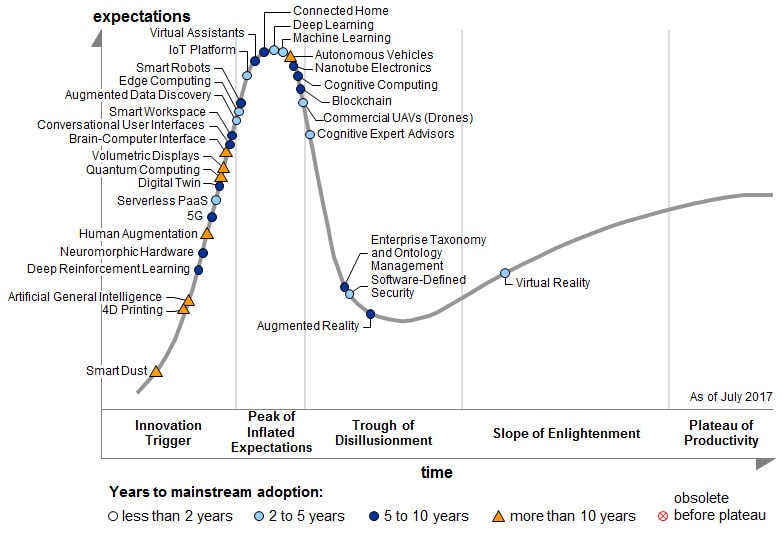
\includegraphics[scale=0.5]{gartner-hype-cycle}
  \caption{Imagen que muestra el "Hype cycle" de Gartner para tecnologías emergentes en 2017.\protect\footnotemark}
  \label{figura-gartner}
\end{figure}

\footnotetext{ \url{https://www.gartner.com/newsroom/id/3784363}, Gartner (July 2017)}

Sin embargo, desde que Apple y Google lanzaran sus respectivas librerías hace apenas un año, la realidad aumentada ha mejorado su situación notablemente, distanciándose de la realidad aumentada vista hasta el momento, estas nuevas librerias permiten, con los componentes de un dispositivo móvil de masas sea posible reconocer y entender el mundo que le rodea, así como su posición en el mundo. Esto supone una diferenciación en las tecnologías hasta entonces presentes, que o bien necesitaban de mucho hardware para ser capaces de conseguir esto, o en dispositivos móviles de masas, tenían capacidades reducidas.\\

Actualmente la realidad aumentada abre un mundo de grandes posibilidades que pueden revolucionar muchos ámbitos, entre ellos el de los juegos, un juego ya no tiene que quedarse dentro de una pantalla o un mundo virtual, ahora puede dar el salto el mundo real, esto aporta un grado de realismo y espectacularidad que puede suponer una reinvención de los juegos como ahora los conocemos.\\

Por otro lado, la mayoría de la población dispone de un dispositivo móvil, como podemos ver en la Figura \ref{figura-ine}, en el año 2017, un 97.4\% de los hogares españoles contaba con al menos un dispositivo móvil \cite{ine}, esto implica que casi la totalidad de los españoles tiene acceso a dispositivos móviles, y por tanto, a las aplicaciones que utilizan realidad aumentada.

\begin{figure}[h]
  \centering
  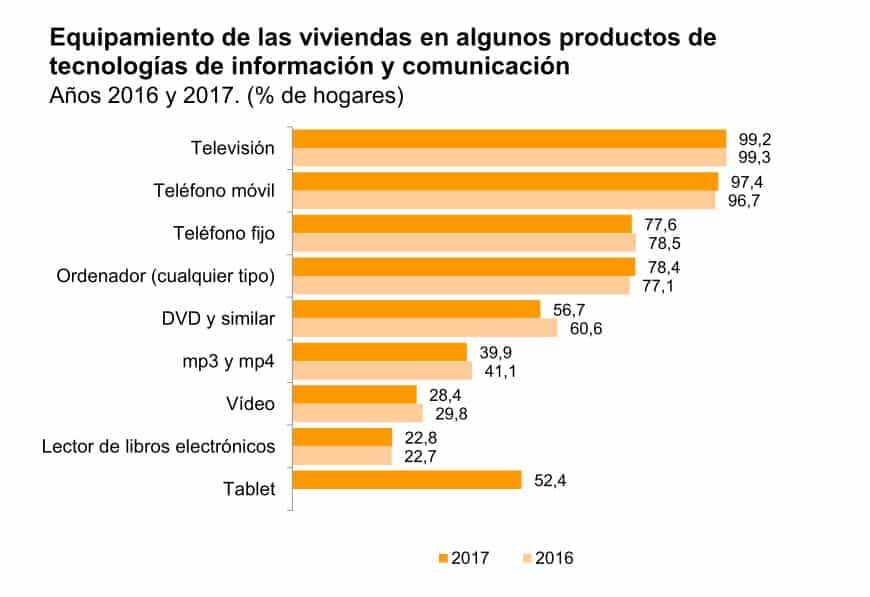
\includegraphics[scale=0.4]{ine2017}
  \caption{Imagen que muestra los porcentajes de hogares que cuentan con cada dispositivo tecnológico.\protect\footnotemark}
  \label{figura-ine}
\end{figure}

\footnotetext{{\em Encuesta sobre Equipamiento y Uso de Tecnologías de la Información y Comunicación en los Hogares.} INE, B. (2017).}

\newpage

\section{Motivación}
Personalmente el estar una gran parte del tiempo de cada dia utilizando mi teléfono móvil y jugando con el me despertó la curiosidad acerca de como se desarrollan los videojuegos, y que es lo que hay detras del producto que al final el usuario descarga de una tienda de aplicaciones.\\

Por otro lado, mi interés por el desarrollo del software me lleva a querer conocer y explorar este mundo, la experiencia de planificar y desarrollar un proyecto software al completo por mi mismo.\\

Las nuevas tecnologías siempre me han llamado la atención y me gusta estar informado sobre ellas, y viendo la revolución de la realidad aumentada me pareció un mundo apasionante por las capacidades ofrece, el poder fusionar el mundo virtual y real, y llevar a cabo aplicaciones y juegos con ella, me pareció algo fascinante y que sin duda me gustaría explorar.\\

La amplia disponibilidad de dispositivos móviles entre la población, y el alto nivel de uso diario que hacen los usuarios de estos, hace del desarrollo para estos dispositivos algo atractivo, ya que es probablemente la mayor plataforma para desarrolladores de software actualmente.\\

Esto en conjunto con el crecimiento de la realidad aumentada, hace que un juego para dispositivos móviles que hace uso de esta tecnología, sea una opción muy interesante para un proyecto, que permite adquirir conocimientos en el desarrollo de videojuegos, en el desarrollo de aplicaciones móviles, y exploarar la realidad aumentada y lo que puede aportar a las aplicaciones de dispositivos móviles actuales.

\section{Estructura del documento}
Este documento se divide en 4 capítulos, a continuación se detalla el contenido de cada uno de los capítulos del documento:
\begin{itemize}
  \item \textbf{Capítulo 1, Introducción y objetivo:} En este capítulo se hace una pequeña introducción al proyecto, explicando la motivación por la que surgió el proyecto, la estructura del documento, y también se exponen los objetivos que han sido establecidos para este proyecto.
  \item \textbf{Capítulo 2, Estado del arte:} En este capítulo se hará una exposición de cual es el estado actual de la realidad aumentada, diferencias con tecnologías similares, que aplicaciones tiene, etc.
  \item \textbf{Capítulo 3, Análisis inicial del problema:} En este capítulo se llevará acabo un analisis de cual es el problema y como este puede ser resuelto.
  \item \textbf{Capítulo 4, Metodologías a usar en el proyecto:} En este capítulo se recogen las diferentes metodologías utilizadas para el desarrollo del proyecto, y se explica como serán utilizadas en el proyecto.
  \item \textbf{Capítulo 5, Plan de entregas:} En este capítulo se detalla el plan de entregas llevado a cabo, y las historias de usuario realizadas para definir los requisitos que tendrá el sistema.
  \item \textbf{Capítulo 6, Desarrollo. Entregas e iteraciones:} En esta capitulo se recogerá el trabajo realizado durante las diferentes iteraciones, así como el resultado de las distintas entregas.
  \item \textbf{Capítulo 7, Conclusiones y Trabajos Futuros:} En este capítulo se recoge el resultado del proyecto, las conclusiones obtenidas del desarrollo de éste y los trabajos futuros a realizar en el proyecto.
\end{itemize}

\section{Objetivo}
El objetivo principal de este proyecto es explorar que ventajas puede aportar la realidad aumentada, mas concretamente el SDK ARCore, a los juegos en dispositivos móviles, y mas específicamente a los juegos de mesa en dispositivos móviles. Por tanto, mediante este proyecto se adquirirá experiencia en el desarrollo con tecnologías de realidad aumentada.\\

Objetivos secundarios:
\begin{itemize}
  \item Investigar una implementación para juegos de mesa virtuales que aporte un enfoque diferente al habitual.
  \item Adquirir conocimientos sobre la planificación y desarrollo de proyectos de software, mas concretamente de videojuegos.
  \item Adquirir conocimientos sobre la realidad aumentada, como ésta funciona y cuales son las mejores SDK para desarrollar utilizando dicha tecnología.
\end{itemize}

\chapter{Objetivos}
\label{ch:objetivos}

\chapter{Metodología de trabajo multidisciplinar}
\label{ch:metodologia}

Este capítulo describe la metodología de trabajo que se ha seguido para llevar a cabo el proyecto. Detalla las tareas y actividades que se planean realizar, así como el conjunto de herramientas de trabajo que se han visto con mayor utilidad para lograr un flujo de trabajo más productivo.\\

Como se mencionó anteriormente, mi tarea consistirá no solo en el desarrollo de una plataforma web, sino también la gestión del equipo, a modo de \textit{project manager}. Como tal, nos encontramos ante la situación de organizar a un equipo de personas que mayormente no son del mismo grado, por lo que pueden no estar acostumbrados o ser conocedores de las mismas herramientas que utlizamos habitualmente.\\

En el presente capítulo se tratará de buscar aquellas herramientas que sean sencillas y tengan una curva de aprendizaje baja. El motivo es múltiple, ya que se han de encontrar recursos aptos para todos, que no los abrumen o les frustren, para que así los utilicen y beneficie al proyecto en si.

\section{Líneas de trabajo}
En el nacimiento de este equipo, se planteó que debemos funcionar de forma similar a una Startup \cite{startup}. Siguiendo esa lógica, trabajamos sobre una idea innovadora para resolver un problema complejo, empleando la tecnología para llegar a cumplir el objetivo.\\

Sobre el concepto de SmartU, nacen una serie de \textbf{líneas de trabajo} que son importantes para lograr un producto completo y útil para su público objetivo, por ello es necesario que se trabaje en ellas de forma correcta.

\begin{description}
    \item[Software] La línea de trabajo donde crear aplicaciones web y móviles que el público objetivo usará con el fin de facilitar la tarea de la creación de proyectos multidisciplinares.
    \item[Marketing] Esta línea de trabajo concentra sus esfuerzos en la búsqueda de formas de promoción adecuadas al público y que garanticen que SmartU llegue al máximo número de personas posibles. Destacamos por ejemplo el uso de las redes institucionales ya existentes para dar difusión, así como la creación de redes sociales propias de la plataforma como forma de acercamiento a los demás.
    \item[Diseño gráfico] La identidad visual es el reto al que se enfrenta esta línea de trabajo. Se ha de encontrar un estilo y diseño diferenciador que además sea agradable al usuario, y que de alguna forma represente los conceptos sobre los que trabajamos, como por ejemplo el concepto principal de ciudades inteligentes.
    \item[Plan de empresa] El plan de empresa tiene como objetivo encontrar una estrategia de negocio que sirva para que esta \textit{startup} sea viable en el futuro.
\end{description}

\section{El equipo}
El equipo de trabajo se ha compuesto de diferentes \textbf{profesores y estudiantes} de diversas disciplinas de la universidad. Podemos ver su nombre y ocupación en la \textbf{tabla \ref{miembrossmartu}}. Todos han aportado conocimientos de su campo al proyecto para intentar lograr los mejores resultados, recibiendo opiniones y puntos de vista muy diferentes que ayudan y complementan.

\begin{table}
    \begin{center}
        \begin{tabular}{|p{4.5cm}|p{6.5cm}|}
            \hline
                \rowcolor{Gray}\multicolumn{1}{|c|}{\textbf{Integrante}}
                & \multicolumn{1}{|c|}{\textbf{Ocupación}} \\
            \hline
                Juan Árbol Gutiérrez & Estudiante de CC.EE. y Empresariales \\
            \hline
                Irene Castillo Pardo & Estudiante de Comunicación y Audiovisuales \\
            \hline
                Emilio Chica Jiménez & Estudiante de Ingeniería Informática \\
            \hline
                Victoria Guerra Molina & Estudiante de Comunicación y Audiovisuales \\
            \hline
                Juan José Jiménez García & Estudiante de Ingeniería Informática \\
            \hline
                Javier Labrat Rodríguez & Estudiante de Ingeniería Informática \\
            \hline
                Germán Zayas Cabrera & Estudiante de Bellas Artes \\
            \hline
                Miguel Gea Megías & Profesor de Ingeniería Informática \\
            \hline
                Guillermo Maraver Tarifa & Profesor de CC.EE. y Empresariales \\
            \hline
                Alejandro Grindlay Moreno & Profesor de Ingeniería Civil \\
            \hline
        \end{tabular}
        \caption{Integrantes del proyecto multidisciplinar SmartU}
        \label{miembrossmartu}
    \end{center}
\end{table}

\subsection{Obligaciones del equipo}
A cada uno de los miembros del equipo se le asigna un rol o tarea. Es importante que cada uno se dedique a algo relacionado con sus conocimientos, de esta manera se esperaba conseguir mejores resultados, al \textbf{delegar en la persona adecuada la tarea adecuada}. Podemos ver el reparto de roles en la \textbf{tabla \ref{rolessmartu}}.\\

\begin{table}
    \begin{center}
        \begin{tabular}{|p{5cm}|p{6cm}|}
            \hline
                \rowcolor{Gray}\multicolumn{1}{|c|}{\textbf{Integrante/s}}
                & \multicolumn{1}{|c|}{\textbf{Rol o tarea}} \\
            \hline
                Juan Árbol Gutiérrez & Emprendedor y gestor de estrategia empresarial \\
            \hline
                Juan José Jiménez García & Gestor de proyecto y desarrollador de software \\
            \hline
                Emilio Chica Jiménez & Gestor tecnológico y desarrollador de software \\
            \hline
                Irene Castillo Pardo y Victoria Guerra Molina & Gestoras de audiovisuales \\
            \hline
                Germán Zayas Cabrera & Diseñador gráfico \\
            \hline
                Javier Labrat Rodríguez, Miguel Gea Megías, Guillermo Maraver Tarifa y Alejandro Grindlay Moreno & Tutores y consultores para dudas \\
            \hline
        \end{tabular}

        \caption{Roles y tareas de los miembros del equipo SmartU}
        \label{rolessmartu}
    \end{center}
\end{table}

En la \textbf{tabla \ref{tareassmartu}} se puede ver un resumen general del trabajo que va a realizar cada uno de los miembros del equipo.

\newpage
\begin{longtable}{|m{4.5cm}|m{6.5cm}|}
    \hline
        \rowcolor{Gray}\multicolumn{1}{|c|}{\textbf{Integrante}}
        & \multicolumn{1}{|c|}{\textbf{Aportaciones}} \\
    \hline
        Juan Árbol Gutiérrez & \begin{itemize}
            \item Organizador del Design Thinking y Brainstorming
            \item Creador del plan estratégico de empresa
            \item Responsable de realización de entrevistas a posibles usuarios objetivo del sistema
            \item Presentador del proyecto en la Facultad de Ciencias de la Actividad Física y del Deporte
        \end{itemize} \\
    \hline
        Irene Castillo Pardo & \begin{itemize}
            \item Colaborador en el Design Thinking y Brainstorming
            \item Creadora del video de presentación del proyecto
            \item Creación del making of del proyecto
        \end{itemize} \\
    \hline
        Emilio Chica Jiménez & \begin{itemize}
            \item Creador de la aplicación móvil del proyecto
            \item Organizador del Design Thinking y Brainstorming
            \item Moderador de seminario de tecnologías emergentes
            \item Gestor de reuniones
        \end{itemize} \\
    \hline
        Victoria Guerra Molina & \begin{itemize}
            \item Colaborador en el Design Thinking y Brainstorming
            \item Investigadora de una campaña de difusión del proyecto en redes sociales y medios de publicidad
        \end{itemize} \\
    \hline
        Juan José Jiménez García & \begin{itemize}
            \item Organizador del Design Thinking y Brainstorming
            \item Gestor del proyecto
            \item Creador de la aplicación web
            \item Coordinador y documentador de reuniones
            \item Coordinador del repositorio de archivos y calendario
        \end{itemize} \\
    \hline
        Javier Labrat Rodríguez & \begin{itemize}
            \item Presentador del proyecto en la Facultad de Ciencias de la Actividad Física y del Deporte
            \item Creador de un proyecto que servirá de muestra para nuestro sistema SmartU
        \end{itemize} \\
    \hline
        Germán Zayas Cabrera & \begin{itemize}
            \item Colaborador en el Design Thinking y Brainstorming
            \item Creador de la identidad visual del proyecto
            \item Creador del diseño de la página web de presentación del proyecto
        \end{itemize} \\
    \hline
        Miguel Gea Megías & \begin{itemize}
            \item Creador de la idea original
            \item Agrupador de los miembros del equipo
            \item Consejero para el desarrollo del proyecto
            \item Colaborador en el Design Thinking y Brainstorming
            \item Gestor de las reuniones
        \end{itemize} \\
    \hline
        Guillermo Maraver Tarifa & \begin{itemize}
            \item Colaborador en el Design Thinking y Brainstorming
            \item Consejero de Juan para el desarrollo del proyecto
            \item Consejero de marketing y promoción del proyecto
        \end{itemize} \\
    \hline
        Alejandro Grindlay Moreno & \begin{itemize}
            \item Colaborador en el Design Thinking y Brainstorming
            \item Consejero para el desarrollo del proyecto
        \end{itemize} \\
    \hline
    \caption{Aportaciones de los miembros del equipo}
    \label{tareassmartu}
\end{longtable}

\subsection{Dependencias entre miembros del equipo}
En un proyecto multidisciplinar, es muy importante \textbf{encontrar sinergias} entre los miembros del mismo, es decir, encontrar puntos comunes que permitan una colaboración fructuosa entre dos personas. Así, el trabajo que teníamos que hacer cada uno se vería más reforzado al contar con el punto de vista y la ayuda proporcionada por otra persona de diferente disciplina.\\\\

Las sinergias son muy populares en el mundo empresarial, en concreto entre los campos de \textit{marketing} o economía, y se valora mucho el resultado obtenido de esa cooperación. Por ello, en este tipo de proyectos, es muy deseable realizar un esfuerzo por encontrarlas.

\section{Gestión del trabajo}
Como gestor del proyecto (una de mis obligaciones además del desarrollo de software), junto con mi tutor Miguel realizaremos la \textbf{organización del trabajo} con el objetivo de conseguir la mayor agilidad posible para la comunicación y para documentar los progresos. En las siguientes secciones de este apartado se describe con más detalle lo que se va a realizar para cada uno de los puntos de gestión.

\subsection{Temporización}
Uno de los aspectos más importante a la hora de gestionar un proyecto es la temporización, es decir, definir los tiempos que se estima requerirán las posibles tareas que surjan para llevarlo a cabo. Es vital tener en mente siempre que los cambios existen y con una alta probabilidad van a aparecer, por lo que se ha de estar preparado para asumirlos e intentar integrarlos en el proyecto, intentando que afecte lo menos posible a la planificación inicial.\\

Para este apartado se puede hacer uso del \textbf{diagrama de Gantt}, que establece tareas y el tiempo requerido de estas, así como los recursos necesarios (tanto humanos como materiales) para poder realizarlas. Permite estudiar mejor posibles bloqueos y dependencias entre tareas, y ver de forma más gráfica si el tiempo se está distribuyendo bien entre integrantes y en el espacio.

\subsection{Comunicación}
Un proyecto de esta índole necesita de varias \textbf{reuniones}, donde poder debatir asuntos y tomar decisiones, así como para realizar ciertas técnicas creativas de generación de ideas y establecer las funcionalidades de los productos a desarrollar. Estos puntos son tratados más adelante en esta documentación.\\

Es deseable que las reuniones sean siempre, en la medida de lo posible, en el mismo lugar, como forma de hacer más estable el proceso del proyecto y no crear demasiada confusión al equipo. De no poder hacer esto posible, se puede intentar hacer uso de instalaciones de la universidad como salas insonorizadas o aulas de seminario, pensadas para trabajos en equipo. Contar con proyector o pizarra en la sala es muy recomendable para hacer una mejor dinámica de reuniones.\\

Debido a la diferencia de disciplinas que presentaban los integrantes, se hace necesario establecer un \textbf{horario semanal} donde se ajuste la disponibilidad de todos los miembros para que puedan asistir el máximo número de personas. Este horario no ha de ser fijo obligatoriamente, semana a semana se puede actualizar para un mejor ajuste a las circunstancias que puedan tener los miembros del equipo.\\

Podemos describir el \textbf{proceso de organización de reuniones} de la siguiente manera:

\begin{enumerate}
    \item Como gestión previa a una reunión, se ha de hacer lo siguiente:
    \begin{enumerate}
        \item Se \textbf{comunica a los gestores} la necesidad de realizar una reunión para tratar un asunto importante del proyecto.
        \item Los gestores se \textbf{reunen} para establecer los puntos de la próxima reunión.
        \item Se \textbf{comunica al resto del equipo} la necesidad de realizar la reunión y se les pide que indiquen en el horario los días que mejor le convenían, para encontrar el punto común para que puedan asistir todos.
        \item Los profesores, debido a la posibilidad que presentan de \textbf{reservar salas de reuniones} más adecuadas que los que los estudiantes tenían permitido, se pueden encargar de encontrar sitio para celebrar la reunión en base a la disponibilidad de los asistentes.\\
        También se pueden encargar de comprobar que la sala que se reserve cuente con material adecuado para la reunión, como un \textbf{proyector, pizarra}, etc.
        \item Se establece en el calendario oficial del proyecto (con \textbf{Google Calendar} \cite{googlecalendar}) y se informaba al resto del equipo por el medio correspondiente.
    \end{enumerate}
    \item Al comenzar la reunión, se han de resumir los puntos tratados en la \textbf{reunión anterior}, a modo de recordatorio y para aquellos miembros que no hubieran podido asistir a dicha reunión. Tras el resumen, se procede a informar de los puntos a debatir en la reunión actual.
    \item Al acabar la reunión se han de comentar los \textbf{nuevos puntos a tratar} de cara a la próxima reunión, y se anotan para no olvidarlos y que los gestores puedan prepararlos.
    \item El gestor del proyecto crea un \textbf{acta de reunión} donde se detallan los puntos debatidos y se apuntan los temas a tratar para la próxima reunión.
\end{enumerate}

Entre las muchas herramientas de comunicación disponibles actualmente, existen algunas muy enfocadas al ámbito profesional, que pueden ser igual de útiles para un entorno de trabajo en equipo universitario. El \textbf{correo electrónico} es un clásico que aun perdura y muchos utilizan, además de aplicaciones de mensajería instantánea como \textbf{WhatsApp}, o el chat de equipos \textbf{Slack}.\\

Se destaca en este punto Slack, al ser una plataforma de comunicación muy pensada para equipos de trabajo de empresas, permitiendo definir canales de comunicación para tratar asuntos concretos, y que agrupen a un subconjunto de personas del equipo, de modo que puedan tratar algo sin molestar al resto de integrantes. Podemos ver una captura de ejemplo de Slack en la imagen \ref{slackimage}.

\begin{figure}
    \centering
    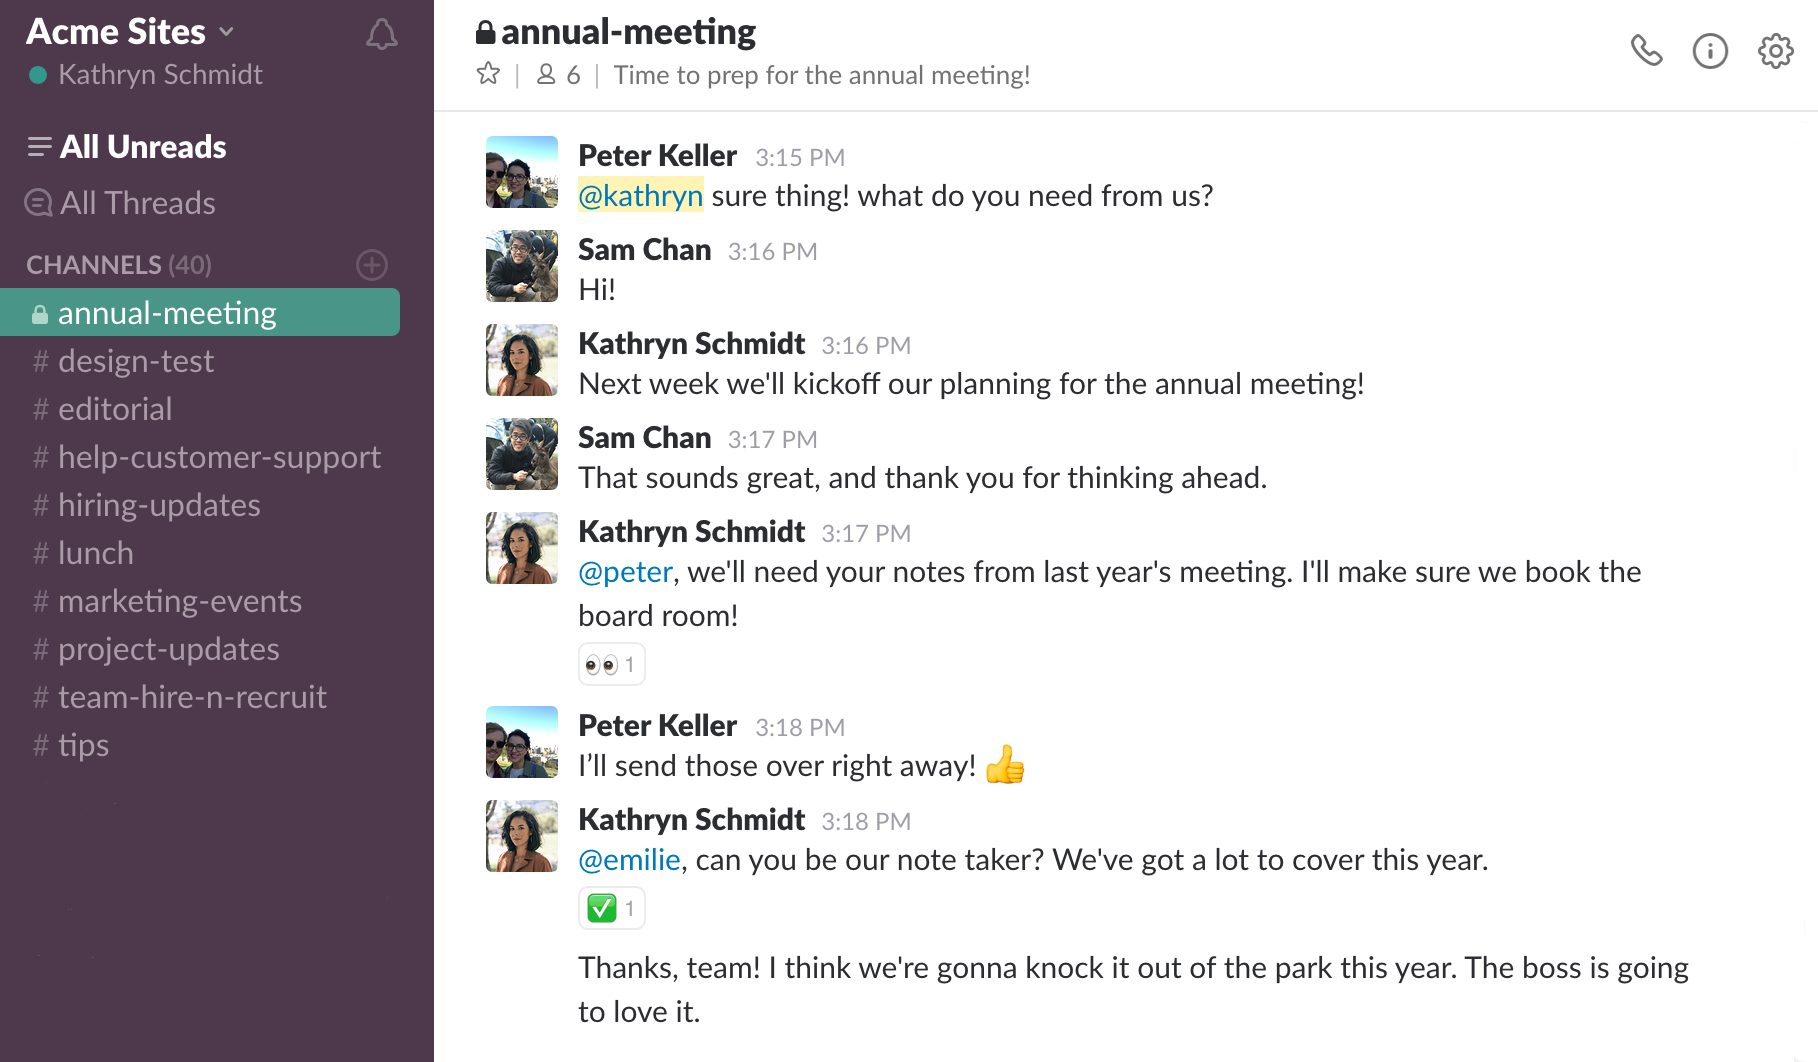
\includegraphics[scale=0.2]{slack}
    \caption{Pantalla principal de Slack - \textcopyright\ Slack}
    \label{slackimage}
\end{figure}

\subsection{Documentación}
Para gestionar la documentación y todo el contenido que el equipo produzca a lo largo del tiempo, es necesario contar con un espacio común de alojamiento de archivos. Para esto se puede optar por utilizar el servicio de almacenamiento en la nube \textbf{Google Drive} \cite{googledrive}.\\

Todos han de tener acceso a dicho directorio online, y ahí se han de ir dejando los documentos que el equipo genere, como pueden ser:
\begin{itemize}
    \item Presentaciones para exponer en reuniones.
    \item Actas de reuniones.
    \item Bocetos de diseño de aplicaciones o de identidad visual.
    \item Calendario semanal actualizado.
\end{itemize}

\subsection{Seminarios y divulgación}
Otro aspecto importante a la hora de realizar un proyecto de este tipo son los seminarios. Los seminarios permiten realizar una presentación y explicación de algún tema o concepto concreto de cualquier área del conocimiento, y generalmente pueden ser para un público más conocedor del tema, o hacerlo más divulgativo para que puedan comprender sus contenidos personas de todos los ámbitos.\\

En un equipo formado por diferentes estudiantes y profesores, es importante dar a conocer conceptos o técnicas habituales en algunas ramas del conocimiento, con el fin de que todos conozcan, no en un nivel avanzado, aspectos importantes para el proyecto, y que a algunos miembros no les resulte extraño o desconocido lo que hacen.\\

Por medio de los seminarios, podemos explicar algo a todo el equipo, y existen diversas técnicas de creatividad que los pueden hacer partícipes en los seminarios, para así motivarlos más y que logren afianzar mejor los nuevos conocimientos.

\subsubsection{Catálogo de seminarios}
Existen multitud de métodos de generación de ideas, que abarcan procesos de análisis, investigación/descubrimiento y definición de estrategias:

\begin{itemize}
    \item Card sorting
    \item Design Thinking
    \item Brainstorming
    \item SCAMPER
    \item Business Model Canvas
\end{itemize}

En esta documentación no vamos a hablar de cada uno de esos métodos, sino que nos centraremos en el que consideramos más interesante y que usaremos en este proyecto, el \textbf{Design Thinking}

\subsubsection{Design Thinking}
Una de las técnicas de creatividad más útiles es la del \textit{Design Thinking}. Tal y como podemos ver en \cite{designthinkinglink}, podemos definirlo como:\\

\textit{``Es un método para generar ideas innovadoras que centra su eficacia en entender y dar solución a las necesidades reales de los usuarios. Proviene de la forma en la que trabajan los diseñadores de producto. De ahí su nombre, que en español se traduce de forma literal como "Pensamiento de Diseño", aunque nosotros preferimos hacerlo como "La forma en la que piensan los diseñadores".''}\\

El Design Thinking es una herramienta muy visual que le da importancia a la experimentación y el prototipado. Su eficacia radica en la capacidad de entender y dar solución a las necesidades reales de los usuarios.\\

Es una técnica muy recomendable y que cada vez se usa más, por lo que es muy recomendable ponerla en práctica con el equipo, ya que puede ser un gran estímulo para obtener ideas, además de que ayuda a que el equipo se conozca mejor y haya más complicidad entre integrantes.

\section{Conclusión}
En este capítulo se han descrito las técnicas y actividades que se pueden realizar para gestionar un equipo multidisciplinar. Los resultados obtenidos tras su aplicación pueden verse en el capítulo \ref{ch:conclusiones}, así como un análisis de los mismos.

\chapter{Proceso de desarrollo}
\label{ch:desarrollo}
Este capítulo abarca mi parte de desarrollo de software de la aplicación web de SmartU. Se describe el análisis y los requisitos que hemos obtenido para este sistema, pasando por el diseño e implementación del mismo. Al final del capítulo se incluye un apartado de herramientas que han sido utilizadas para el desarrollo de este software.

\section{Introducción}
Al comenzar el desarrollo, se pudo apreciar que había una alta posibilidad de sufrir cambios a lo largo del proceso debido a que el alcance del mismo no estaba muy delimitado. Es por ello que se optó por seguir una metodología principalmente ágil, la cual permitía mayor flexibilidad y facilidad para adaptar posibles cambios.\\

En el desarrollo ágil es importante la comunicación entre todos los miembros del equipo y que éstos, de alguna forma, participen activamente durante el desarrollo. No todos los miembros de este equipo multidisciplinar trabajan en el ámbito de la Ingeniería Informática, pero sabíamos que podían colaborar en las primeras fases aportando ideas y posibles requisitos. Sin embargo, sí que era importante que hubiera comunicación y consenso entre los miembros del área de Informática. Con mi compañero Emilio se realizó una puesta en común para intentar unificar las plataformas que cada uno teníamos que desarrollar.\\

Siguiendo algunos de los principios del desarrollo ágil, se ha evitado realizar documentación innecesaria, y se ha optado por ir a lo primordial y esencial, sin que ello repercuta en la calidad del software. Hay que tener en cuenta que este desarrollo pretende ser continuado y mejorado en el tiempo, por lo que una documentación base correcta es importante.\\

Por último, añadiremos que se ha preferido optar por establecer una lista de requisitos del sistema en lugar de emplear la técnica de las \textbf{historias de usuario}, ya que no son de obligado cumplimiento el desarrollarlas, y se ha de tener en cuenta el hecho de que el desarrollo será continuado por otras personas en el futuro.

\section{Análisis}
La fase de análisis se distribuye en \textbf{dos grandes bloques}:

\begin{itemize}
    \item El primer bloque comprende el análisis en equipo del problema y la extracción de unos primeros requisitos y usuarios base sobre los que basaremos nuestras decisiones futuras a la hora de desarrollar el sistema. Aquí se realizarán diversas técnicas de generación de ideas y prototipado para acotar y definir mejor el sistema.
    \item El segundo bloque es más habitual del proceso de desarrollo de software, ya que se va a dedicar a recopilar y mostrar los requisitos del sistema ya definidos correctamente, tras haber terminado el análisis del primer bloque.
\end{itemize}

\subsection{Generación de ideas y extracción de requisitos}
Tal y como se describió en el capítulo \ref{ch:metodologia}, es importante realizar sesiones de generación de ideas para empezar a recopilar ideas para el desarrollo. Se realizó un seminario sobre tecnologías emergentes, y otro sobre \textit{Design Thinking/Brainstorming}. Esto se describe con más detalle en el capítulo \ref{ch:conclusiones}.\\

Más adelante se obtuvo más información gracias a la presentación del proyecto multidisciplinar que se hizo en la Facultad de Ciencias de la Actividad Física y del Deporte, realizada por los compañeros Javier y Juan. Allí se pudo enseñar el proyecto a potenciales usuarios (\textit{stakeholders}) y recibimos opiniones muy interesantes de posibles características que les gustaría ver para que fuese una aplicación web más completa y funcional.

\subsubsection{Usuarios del sistema}
Tras las reuniones de generación de ideas, se llegó a la siguiente conclusión respecto a \textbf{quiénes son los usuarios potenciales del sistema}. Es importante poder definir a los posibles futuros usuarios de nuestra aplicación para así poder enfocar mejor los requisitos y el diseño de nuestra aplicación web. Nuestro equipo en si consta de algunos de ellos: son los estudiantes y profesores, o en general, la comunidad educativa.

\begin{itemize}
    \item Los \textbf{estudiantes} son potenciales usuarios registrados de nuestra aplicación web. Podemos concretar más e irnos al segmento de estudiantes de último año de grado o máster que necesitan una idea para realizar un proyecto de final de grado/máster, pero también están aquellos estudiantes que cuentan con una idea para un proyecto y necesitan a otros estudiantes con los que conformar un equipo.\\
    Este grupo de usuarios es el que se prevee que sería el que utilizase el sistema con mayor frecuencia.
    \item Otro segmento de usuarios es los \textbf{habitantes de la ciudad}. La diferencia radica en que por lo general, es un colectivo no asociado a la universidad y desconocedor de lo que ocurre dentro de ésta. Por ello, no son considerados potenciales usuarios que se van a registrar en el sistema, pero si entrarán y consultarán las ideas que se han publicado.\\
    Pueden ser participantes activos de un proyecto que se esté creando si éste es un proyecto que le interese o afecte a su entorno (barrio, movilidad, economía, etc).
    \item Por último, tenemos el grupo de \textbf{usuarios empresarios}. Estos son aquellas personas que, o bien tienen una idea, o encuentran interesante una idea que han visto publicada en la aplicación. Pueden ponerse en contacto con un equipo de un proyecto y ayudarles con financiación o promoción de su idea, entre otras posibilidades.
\end{itemize}

Para representar de una forma más visual a estos usuarios, se han creado una serie de bocetos de usuario (o \textit{User Persona}), que esquematizan y ayudan a definir de un vistazo el tipo de perfil de usuario que hemos definido. Podemos verlos en las figuras \ref{usuario_estudiante}, \ref{usuario_ciudadano} y \ref{usuario_empresario}.\\

Como podemos ver, el conjunto de potenciales usuarios intenta abarcar a todo el conjunto de la población, por lo que una buena implantación del mismo podría \textbf{reportar enormes beneficios} para todos ellos, ya sea encontrando un proyecto en el que trabajar, como llevar a cabo una idea que mejore la vida en general de los ciudadanos.

\begin{figure}
    \centering
    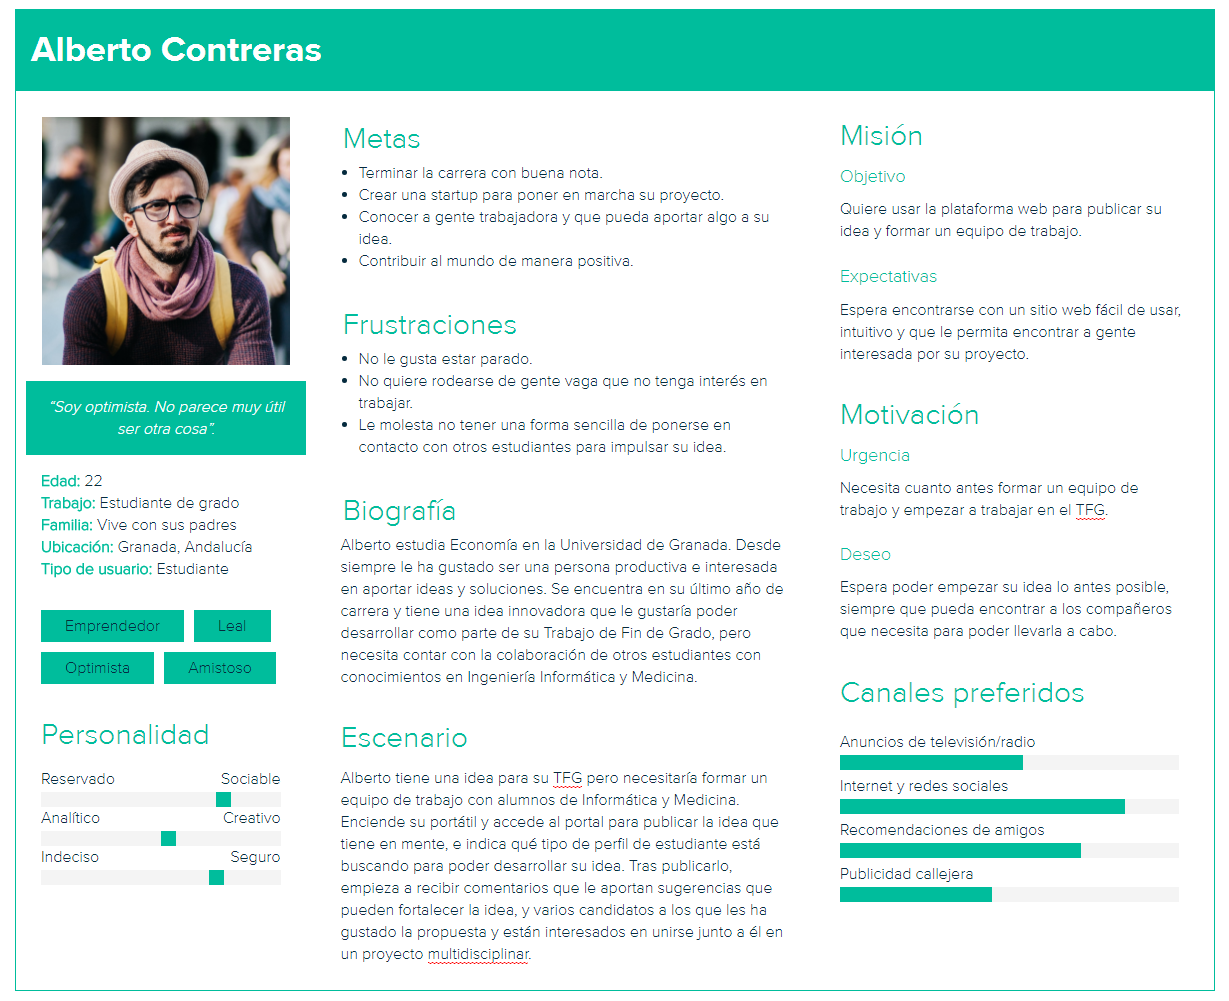
\includegraphics[scale=0.275]{usuario_estudiante}
    \caption{\textit{User Persona} de un estudiante}
    \label{usuario_estudiante}
\end{figure}

\begin{figure}
    \centering
    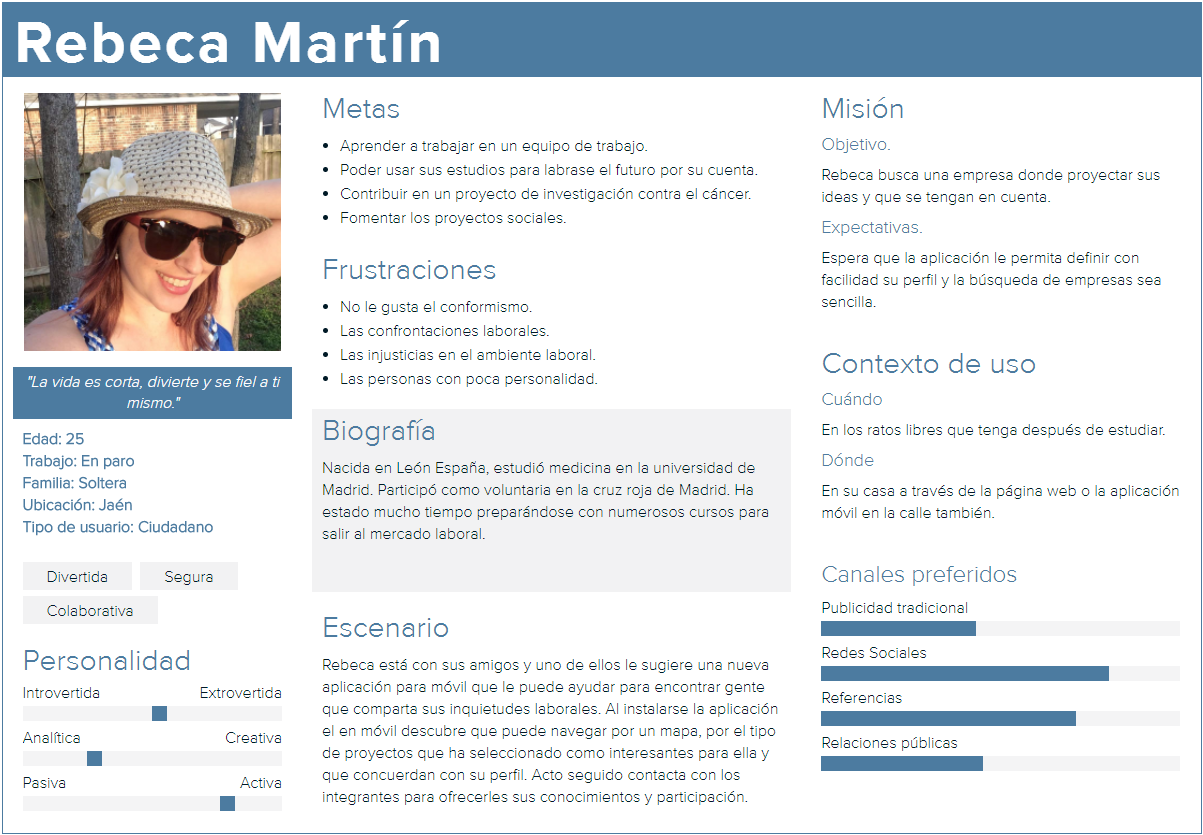
\includegraphics[scale=0.275]{usuario_ciudadano}
    \caption{\textit{User Persona} de un ciudadano}
    \label{usuario_ciudadano}
\end{figure}

\begin{figure}
    \centering
    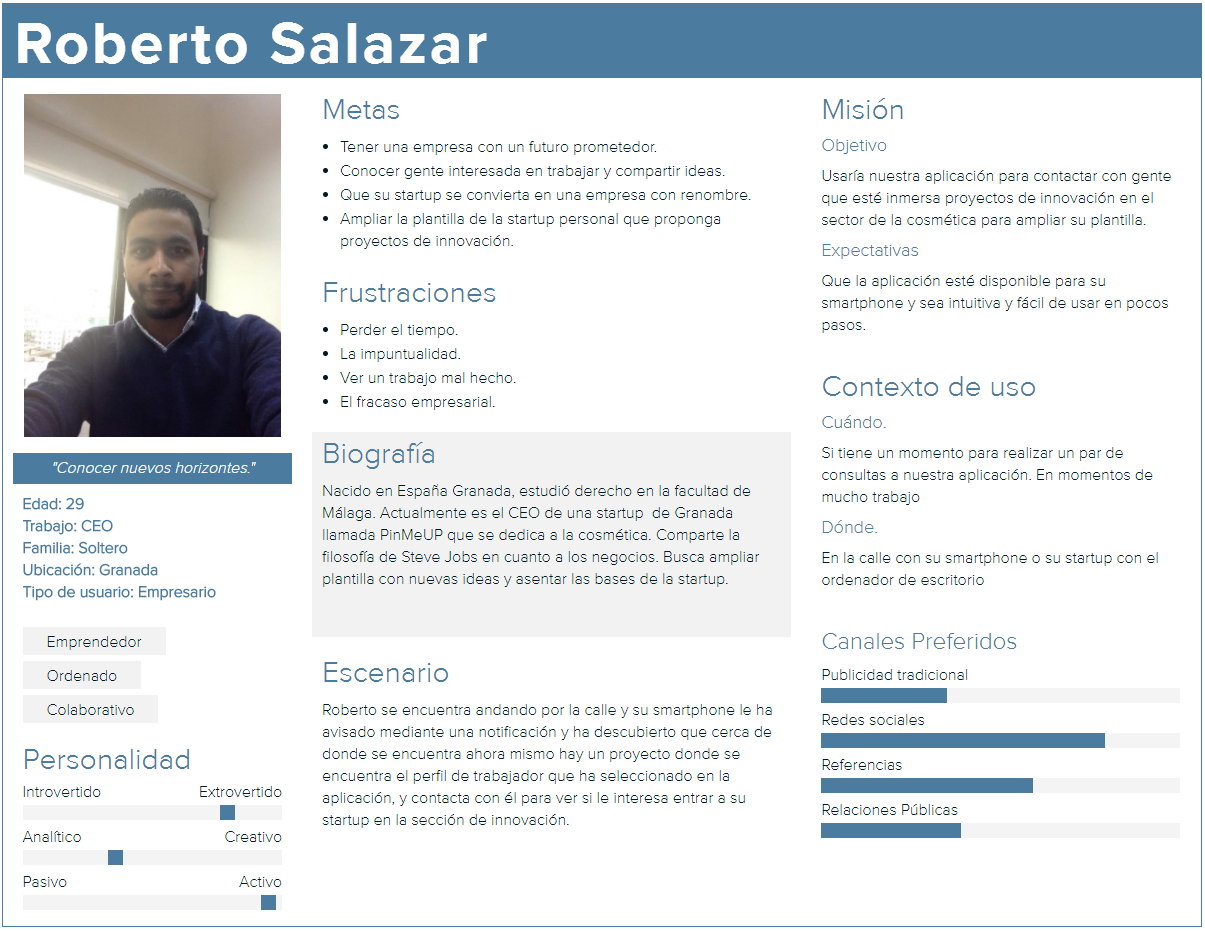
\includegraphics[scale=0.275]{usuario_empresario}
    \caption{\textit{User Persona} de un empresario}
    \label{usuario_empresario}
\end{figure}

\subsection{Requisitos del sistema}
En base a todas las reuniones e información recabada de las mismas y de posibles stakeholders, se ha confeccionado la siguiente lista de requisitos del sistema.

\subsection*{Requisitos de datos}
Se quiere implementar un sistema de información basado en web que sea capaz de almacenar la información relativa a proyectos para la universidad, permitiendo la asignación de información más detallada como área de conocimiento del proyecto, descripción y avances del mismo, así como la información perteneciente a los usuarios que se registren en la plataforma, sus comentarios e información de perfil.

\begin{description}
    \item[RD1. Proyecto:] Un proyecto necesita almacenar la siguiente información:
        \begin{description}
            \item[Nombre:] Cadena de caracteres.
            \item[Descripción:] Cadena de caracteres.
            \item[Página web:] Cadena de caracteres.
            \item[Localización:] Cadena de caracteres.
            \item[Coordenadas:] Cadena de caracteres.
            \item[Fecha de creación:] Fecha de alta del proyecto en el sistema.
            \item[Fecha de eliminación:] Fecha estimada de finalización del proyecto.
            \item[Fecha de actualización:] Fecha de última actualización del proyecto.
            \item[Propietario:] Identificador del usuario registrado que creó el proyecto.
            \item[Imagen destacada:] Cadena de caracteres del nombre de un archivo de imagen.
        \end{description}
    \item[RD2. Redes sociales:] Los proyectos y los usuarios pueden definir sus propias redes sociales para darse a conocer, y necesitan la siguiente información:
        \begin{description}
            \item[Nombre:] Cadena de caracteres.
            \item[URL:] Cadena de caracteres.
            \item[ID de usuario:] Identificador del usuario.
            \item[ID del proyecto:] Identificador del proyecto.
        \end{description}
        Una red social petenece a un usuario o a un proyecto, se han unificado para evitar redundancia.
    \item[RD3. Área del proyecto:] Los proyectos tienen una o varias áreas, y se necesita la siguiente información para poder guardarlas.
        \begin{description}
            \item[Nombre:] Cadena de caracteres.
            \item[Descripción:] Cadena de caracteres.
        \end{description}
    \item[RD4. Buena Idea:] Una buena idea se asemeja a un ``Me gusta'' de redes como Facebook o Twitter. Necesita la siguiente información:
        \begin{description}
            \item[ID del proyecto:] Identificador del proyecto.
            \item[ID del usuario:] Identificador del usuario.
            \item[Tipo:] Indica el tipo de recurso al que se le da ¡Buena Idea!, pensado para ampliar esta funcionalidad a otro tipo de recursos.
            \item[Borrado:] Indica si el ¡Buena Idea! dado se quitó o no.
        \end{description}
    \item[RD5. Especialidad:] La especialidad es algo a lo que un usuario se dedica o que tiene experiencia en ello. Sirve para encontrar a gente de un determinado campo que necesita un proyecto. Se necesita la siguiente información:
        \begin{description}
            \item[Nombre:] Cadena de caracteres.
            \item[Descripción:] Cadena de caracteres.
        \end{description}
    \item[RD6. Experiencia en especialidad:] Partiendo del requisito de dato anterior, un usuario cuenta con un cierto nivel de experiencia en una especialidad, lo cual requiere almacenar la siguiente información:
        \begin{description}
            \item[Experiencia:] Cadena de caracteres.
            \item[ID de la especialidad:] Identificador de la especialidad.
            \item[ID del usuario:] Identificador del usuario.
        \end{description}
    \item[RD7. Comentario:] Los usuarios registrados pueden dejar comentarios en sus proyectos o en los de otros usuarios. Se necesita la siguiente información:
        \begin{description}
            \item[Contenido:] Cadena de caracteres.
            \item[Fecha de creación:] Fecha insertada cuando se creó el comentario.
            \item[ID del usuario:] Identificador del usuario que hace el comentario.
            \item[ID del proyecto:] Identificador del proyecto donde se comenta.
        \end{description}
    \item[RD8. Avance:] Un proyecto puede tener un conjunto de avances que muestre a los usuarios el progreso que se está logrando con el proyecto. Necesita la siguiente información:
        \begin{description}
            \item[Nombre:] Cadena de caracteres.
            \item[Descripción:] Cadena de caracteres.
            \item[Fecha de creación:] Fecha de publicación del avance
            \item[Imagen destacada:] Cadena de caracteres del nombre de un archivo de imagen.
            \item[ID del proyecto:] Identificador del proyecto al que va asociado.
        \end{description}
    \item[RD9. Vacante:] Una vacante representa una disponibilidad de un puesto, en una determinada disciplina, como integrante en un proyecto. Se necesita la siguiente información:
        \begin{description}
            \item[Experiencia:] Una cadena de caracteres.
            \item[Especialidad:] Un identificador de una especialidad concreta.
        \end{description}
    \item[RD10. Hashtag:] Uno o varios proyectos pueden tener etiquetas conocidas como \textit{hastags}, y se necesita guardar para ello:
        \begin{description}
            \item[Nombre:] Una cadena de caracteres.
        \end{description}
    \item[RD11. Usuario:] Un usuario necesita almacenar la siguiente información:
        \begin{description}
            \item[Nombre:] Cadena de caracteres.
            \item[Apellidos:] Cadena de caracteres.
            \item[Email:] Cadena de caracteres.
            \item[Contraseña:] Cadena de caracteres.
            \item[Biografía:] Cadena de caracteres.
            \item[Página web:] Cadena de caracteres.
            \item[Localización:] Cadena de caracteres.
            \item[Puntos:] Número entero.
            \item[CIF:] Cadena de caracteres.
            \item[Admin:] Booleano.
            \item[Verificado:] Booleano.
            \item[Avatar:] Cadena de caracteres del nombre de un archivo de imagen.
        \end{description}
    \item[RD12. Solicitud colaboración:] Los usuarios pueden solicitar colaborar en un proyecto que tenga vacantes disponibles. Se necesita almacenar la siguiente información:
        \begin{description}
            \item[Fecha:] Fecha de creación de la solicitud.
            \item[Descripción:] Una cadena de caracteres.
            \item[Usuario solicitante:] Identificador del usuario que solicita colaborar.
            \item[Proyecto solicitado:] Identificador del proyecto en el que se desea colaborar.
        \end{description}
    \item[RD13. Colaborador:] Un usuario puede ser colaborador de un proyecto en una determinada especialidad. Se necesita almacenar:
        \begin{description}
            \item[ID del usuario:] Identificador del usuario colaborador.
            \item[ID del proyecto:] Identificador del proyecto donde colabora.
            \item[ID de especialidad:] Identificador de la especialidad del colaborador.
        \end{description}
    \item[RD14. Intereses:] Los usuarios pueden marcar intereses en determinadas áreas. Para ello se necesita guardar:
        \begin{description}
            \item[ID del usuario:] Identificador del usuario que marca un interés.
            \item[ID del área:] Identificador del área donde el usuario marca un interés.
        \end{description}
    \item[RD15. Status:] Un ususario puede tener un status en base a su participación en la aplicación web, por ejemplo publicando proyectos o bien dando ``Buena Idea'' a otros. Se requiere la siguiente información:
        \begin{description}
            \item[Nombre:] Cadena de caracteres. Es el nombre que recibe el status.
            \item[Puntos:] Número entero que representa los puntos que se han de alcanzar para llegar a dicho status.
        \end{description}
    \item[RD16. Seguidor:] Un usuario puede seguir a otro para estar al tanto de sus proyectos y de lo que hace en la aplicación web. Se necesita almacenar lo siguiente:
        \begin{description}
            \item[ID del usuario seguido:] Identificador del usuario al que se sigue.
            \item[ID del usuario seguidor:] Identificador del usuario que está siguiendo.
        \end{description}
\end{description}

\subsection*{Restricciones semánticas}
\begin{description}
    \item[RS1.] Un usuario no registrado no puede participar en la aplicación web salvo para consultar la información.
    \item[RS2.] Un usuario no puede tener el mismo email o nombre de usuario que otro registrado anteriormente.
    \item[RS3.] Un proyecto solo puede tener un usuario propietario.
    \item[RS4.] Los usuarios solo pueden modificar o eliminar proyectos de los que son propietarios.
    \item[RS5.] Un usuario puede solicitar unirse al proyecto si hay vacantes y si no es ya propietario o colaborador.
    \item[RS6.] Un usuario no puede seguirse a sí mismo.
    \item[RS7.] Un usuario no puede dar Buena Idea a su/s propio/s proyecto/s.
    \item[RS8.] Los usuarios con correo corporativo reconocido serán registrados automáticamente como usuarios ``verificados''.
\end{description}

\subsection*{Requisitos funcionales}
\subsubsection{Requisitos funcionales de inserción}
\begin{description}
    \item[RF1. Registrar usuario:] un usuario invitado puede registrarse en el sistema para poder utilizar el resto de funcionalidades.
    \item[RF2. Crear proyecto:] Un usuario registrado puede crear un nuevo proyecto en el sistema para dar a conocer su idea.
    \item[RF3. Dar Buena Idea:] Un usuario puede dar un Buena Idea a un proyecto
    \item[RF4. Dejar un comentario:] Un usuario registrado puede dejar un comentario en un proyecto.
    \item[RF5. Elegir áreas de interés:] Un usuario registrado puede seleccionar una o más áreas que sean de su interés para encontrar proyectos afines.
    \item[RF6. Seguir a un usuario:] Un usuario registrado en el sistema puede seguir a otro usuario para estar al tanto de su actividad en la aplicación.
    \item[RF7. Crear vacante:] Un usuario propietario de un proyecto puede crear una vacante para buscar colaboradores para su proyecto.
    \item[RF8. Solicitar colaboración:] Un usuario puede solicitar colaborar en un proyecto que no sea suyo si éste tiene una vacante disponible.
    \item[RF9. Insertar avance:] Un usuario propietario de un proyecto puede crear un avance de un proyecto que muestre algun tipo de progreso.
    \item[RF10. Insertar nuevo colaborador:] Un usuario propietario de un proyecto puede aceptar o rechazar una petición de colaboración para una vacante.
\end{description}

\subsubsection{Requisitos funcionales de consulta}
\begin{description}
    \item[RF11. Listar solicitudes:] Un usuario propietario de un proyecto puede listar las solicitudes de colaboración en su proyecto pendientes de aprobación.
    \item[RF12. Listar vacantes:] Cualquier usuario puede listar las vacantes existentes para un proyecto.
    \item[RF13. Listar avances:] Cualquier usuario puede listar los avances realizados en un proyecto.
    \item[RF14. Listar proyectos:] Cualquier usuario puede listar los proyectos existentes en la aplicación.
    \item[RF15. Listar usuarios:] Cualquier usuario puede listar usuarios registrados en la aplicación.
    \item[RF16. Listar comentarios:] Cualquier usuario puede listar los comentarios de un proyecto.
    \item[RF17. Listar áreas:] Cualquier usuario puede listar las áreas disponibles en el sistema.
    \item[RF18. Listar colaboradores:] Cualquier usuario puede listar los colaboradores actuales de un proyecto.
    \item[RF19. Consultar detalles de un proyecto:] Cualquier usuario puede ver los detalles de un proyecto.
    \item[RF20. Consultar detalles de un usuario:] Cualquier usuario puede ver el perfil de otro usuario registrado en la aplicación.
\end{description}

\subsubsection{Requisitos funcionales de eliminación}
\begin{description}
    \item[RF21. Eliminar áreas de interés:] Un usuario registrado puede modificar su perfil y eliminar una o varias áreas que sean de su interés.
    \item[RF22. Eliminar Buena Idea de un proyecto:] Un usuario puede eliminar el Buena Idea que le ha dado a un proyecto.
    \item[RF23. Dejar de seguir a un usuario:] Un usuario registrado puede dejar de seguir a otro usuario registrado en el sistema.
\end{description}

\subsection*{Requisitos no funcionales}
\begin{description}
    \item[RNF1.] La aplicación web debe estar finalizada para septiembre de 2017.
    \item[RNF2.] La aplicación web debe tener un diseño adaptable a todo tipo de tamaños de pantalla de dispositivo.
    \item[RNF3.] La aplicación web debe funcionar correctamente en la mayoría de navegadores de Internet más utilizados y en sus últimas versiones disponibles.
    \item[RNF4.] El código de la aplicación debe estar correctamente comentado para facilitar la tarea de mejorarlo a los futuros desarrolladores que continúen el proyecto.
\end{description}

\section{Diseño e Implementación}
Tras el proceso de análisis de nuestro sistema y extracción de los requisitos que necesitaría nuestra aplicación web, procedemos a describir los principales aspectos de diseño e implementación de la misma, incidiendo en aspectos importantes e inherentes al proceso de desarrollo de un sistema de información web.\\

La codificación de la aplicación web de SmartU venía condicionada por la necesidad de un desarrollo que fuese agilizado e iterativo, intentando completar funcionalidades específicas en cada \textit{``paso''} que se diese a lo largo de este proceso. Esto me llevó a tomar una serie de decisiones respecto al lenguage de programación que utilizaría, así como el conjunto de herramientas que me ayudarían con esta tarea, pero siempre teniendo como máxima un desarrollo correcto y bien realizado.

\subsection{Laravel}
Para este proyecto, opté por el framework \textbf{Laravel} \cite{laravel}. La elección del mismo no fue fácil, y llevó algo de tiempo debido al análisis de pros y contras que podría encontrarme a lo largo del proceso de desarrollo. Existen numerosos lenguages de programación como Python, JavaScript, Java, etc, todos con diferentes soluciones de desarrollo web. En el caso de Laravel, se basa en el lenguage PHP, que es ya bien conocido en el mundo de la programación web, y a lo largo de los años ha ido mejorando su potencial con nuevas versiones que incorporaban características que si estaban presentes en otros lenguages.\\

Laravel es un framework de desarrollo web basado en PHP creado por Taylor Otwell en el año 2011. Fue creado con el intento de proporcionar una alternativa más avanzada a \textbf{CodeIgniter}. En muchos lugares de Internet, Laravel es conocido por darle un muy necesitado lavado de cara a PHP, y hacerlo de nuevo más atractivo a la vista de los desarrolladores.\\

Laravel agiliza los procesos en casi todos los apartados existentes del desarrollo de una aplicación web. Proporciona un conjunto de herramientas para gestionar la autenticación de usuarios, bases de datos rutas, entre otros elementos que a continuación se detallan:

\begin{itemize}
    \item Está basado en el conocido patrón de diseño MVC \textbf{(Modelo-Vista-Controlador)}, lo cual permite separar la lógica de nuestra aplicación de la interfaz de usuario, usando como intermediario un controlador que mueva los datos entre modelos y vistas. Con esta idea en mente es fácil obtener un diagrama de clases general del sistema, como el que podemos ver en la imagen \ref{diagramaclases}.
    \item Cuenta con soporte para \textbf{Composer}, lo cual nos permite gestionar de forma sencilla las dependencias de nuestro proyecto, por ejemplo para realizar el despliegue.
    \item Al estar basado en PHP, contamos con el extenso conjunto de funciones que ya nos proporciona el lenguage. Para los programadores actuales de PHP, empezar a usar Laravel \textbf{no supone un mayor esfuerzo}, ya que usa todos los elementos y sintaxis del mismo.
    \item Cuenta con un motor de plantillas, \textbf{Blade}, que permite construir la interfaz web de forma dinámica, recibiendo datos como parámetros y utilizarlos para mostrar la información al usuario.
    \item Laravel dispone de una \textbf{extensa comunidad} de desarrolladores que proporcionan consejos y soluciones a los diversos problemas que puedan surgir a la hora de desarrollar con este framework. En este sentido es fácil encontrar la respuesta a cualquier duda, lo cual hace que el aprendizaje sea mucho más sencillo.
\end{itemize}

\begin{figure}
    \centering
    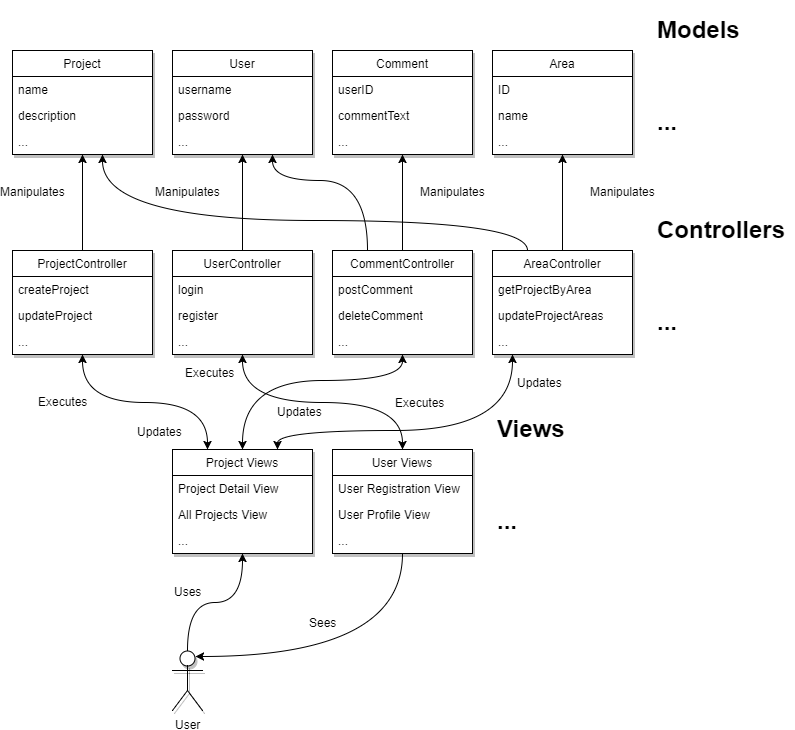
\includegraphics[scale=0.6]{diagramaclases}
    \caption{Diagrama de clases general del sistema}
    \label{diagramaclases}
\end{figure}

La razón por la que elegí este framework era por la sencillez con la que resolvía muchos de los aspectos técnicos que esta aplicación web necesita, además de que se basa en un lenguage de programación que conozco. Siempre es importante estar al tanto de las novedades en los lenguages de programación, pero cuando el tiempo es una restricción muy importante, se hace necesario usar soluciones basadas en algo que ya se conoce. Además, la documentación de este framework es bastante extensa, y cuenta con diversas guías y tutoriales, lo que agillizó bastante su manejo y aprendizaje \cite{laraveldocs}.

\subsection{Estructura del proyecto}
El proyecto se divide en una serie de carpetas generadas automáticamente al crear un nuevo proyecto de Laravel. El código logra una mayor legibilidad y mantenibilidad al separar en diferentes directorios la arquitectura de nuestra aplicación web. En la figura \ref{directorios} podemos ver la estructura completa de ficheros y carpetas, destacando las siguientes:

\begin{description}
    \item [App] En esta carpeta encontramos toda la \textbf{lógica} de nuestra aplicación. Alberga todos los controladores y modelos de datos, así como otros conjuntos de clases que el framework utiliza para poder funcionar. También podemos destacar otros elementos como los \textbf{\textit{Requests}} o los \textbf{\textit{Middlewares}}, pero hablaré de ellos más adelante.
    \item [Config] La carpeta de configuración de nuestro proyecto. En ella se encuentran muchas variables que permiten ajustar la base de datos que vamos a usar, el idioma por defecto de la aplicación, la zona horaria, entre otros muchos aspectos.
    \item [Database] En esta carpeta alojamos todo lo relativo a la base de datos. Principalmente tenemos las \textbf{migraciones} y los \textbf{\textit{seeders}}, y permiten establecer las tablas y columnas que necesitaremos. Hablaremos también de estos aspectos más adelante.
    \item [Public] La carpeta public es el \textbf{punto de inicio} de nuestra aplicación web. Es el único sitio que es visible para los usuarios, o dicho de otra manera, la única carpeta que el servidor web puede ``ver''.
    \item [Resources] Esta carpeta contiene todo lo relacionado con la vista. Incluye carpetas para las diferentes \textbf{plantillas} de la aplicación, ficheros de \textbf{lenguage}, así como archivos de \textbf{hojas de estilo} y scripts. Más adelante hablaremos de este punto.
    \item [Routes] Esta carpeta contiene las rutas de nuestra aplicación. Permite definir URLs que el usuario puede introducir en su navegador, y cada una dará lugar a una acción diferente, como puede ser mostrar la página de inicio o subir un nuevo proyecto al servidor. Las rutas hacen un uso completo de los verbos de HTTP como \textbf{GET}, \textbf{POST}, \textbf{DELETE}, \textbf{UPDATE}, etc.
\end{description}

\begin{figure}
    \centering
    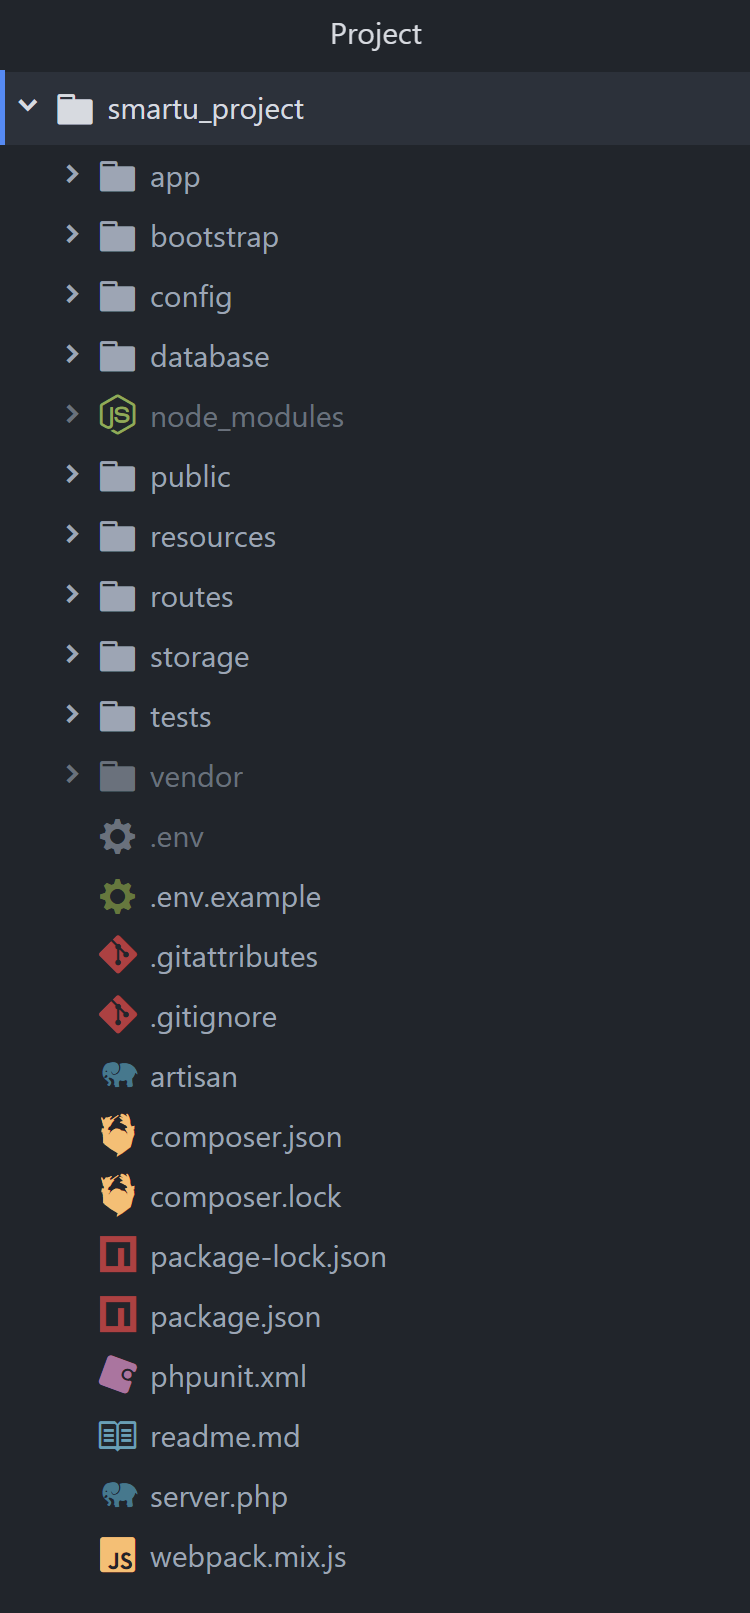
\includegraphics[scale=1.25]{directorios}
    \caption{Estructura de carpetas y ficheros del proyecto}
    \label{directorios}
\end{figure}

\subsection{Middlewares}
Laravel hace un extenso uso de los \textit{Middlewares}. Podemos definirlos como software intermediario que proporciona una capa de abstracción entre una aplicación y otra. En el caso de Laravel, nos proporciona por defecto una serie de middlewares que realizan varias tareas sin que nosotros tengamos que intervenir en ellas, liberando al programador de carga de trabajo.\\

Uno de los principales middleware que proporciona este framework es el de autenticación. Permite, por ejemplo, que un usuario autentificado en el sistema pueda realizar ciertas tareas y evita que aquellos que no lo están las puedan hacer, en cuyo caso los redigire a otra dirección que si tengan permitida. Otro middleware importante es el de la verificación del token CSRF, pero esto lo hablaremos con más detalle en el apartado de seguridad.

\subsubsection{Middleware de localización}
Con el objetivo de lograr que la aplicación web tuviera soporte \textbf{multilenguaje}, se ha hecho uso de un middleware personalizado que captura los parámetros de la URL y detecta si existe un código de idioma correcto, y en caso de no tenerlo, le añade el del idioma por defecto de la aplicación. Como se puede comprobar, los middlewares nos permiten delegar ciertas tareas para no tener que preocuparnos de nada y poder continuar el desarrollo.

\subsection{Patrones de diseño}
El uso de patrones de diseño es muy recomendable a la hora de desarrollar software. Laravel, por su funcionamiento interno, logra aplicar el patrón MVC mencionado anteriormente, pero no es el único que encontramos. Existen más patrones de diseño que se aplican para determinadas características, como por ejemplo:

\begin{description}
    \item [Builder] El patrón Builder permite separar la creación de un objeto complejo de su representación, con el fin de que el mismo proceso de construcción pueda usarse para crear diferentes representaciones. En Laravel podemos tomar como ejemplo la clase \textit{AuthManager}, que hereda de \textit{Manager}, siendo esta última la clase Builder que se encarga de construir los componentes seguros necesarios para almacenar informaciónde autentificación, ya sea en una variable de sesión o en una cookie.
    \item [Factoría] Este patrón permite definir una interfaz común de creación de objetos, pero deja a las subclases que sean ellas las que decidan qué objeto es el que quieren instanciar. Laravel hace un extenso uso de este patrón, por ejemplo, a la hora de crear conjuntos de reglas de validación de datos (usados habitualmente para comprobar los que se reciben a través de un formulario).
    \item [Estrategia] El patrón Estrategia o también conocido como \textit{Policy}, define una familia de algoritmos y los encapsula cada uno, haciendo que estos puedan ser reutilizados en cualquier momento.
    \item [Fachada] El patrón Fachada proporciona una interfaz unificada a un conjunto de interfaces de un subsistema. La fachada define una interfaz de alto nivel que hace que el subsistema sea más sencillo de usar. Laravel está construido con el uso de este patrón en casi todas partes, agrupando funcionalidades complejas en unas más simples de usar.
\end{description}

\section{Pruebas}
Para realizar la fase de pruebas de este proyecto, se ha seguido el proceso habitual de una \textbf{metodología ágil}, es decir, probar que las funcionalidades de la aplicación web funcionan correctamente en todos los posibles casos de uso. En concreto, se ha seguido el siguiente proceso:

\begin{itemize}
    \item El desarrollo se ha realizado implementando en primer lugar las \textbf{funcionalidades \textit{core}} o ensenciales de la aplicación, es decir, la gestión de los usuarios y los proyectos, así como la gestión de los diferentes idiomas que pueda haber disponibles.\\
    Se ha garantizado mediante pruebas que en este punto es posible crear usuarios y proyectos, y los usuarios invitados (no registrados) sólo pueden hacer operaciones de consulta.\\
    También se ha garantizado que el cambio de idioma de la aplicación se hace correctamente.
    \item Tras la funcionalidad esencial, se han implementado las \textbf{pequeñas funcionalidades} que no presentan un fuerte acoplamiento con otras y que no dependen del funcionamiento de éstas, de modo que se puede garantizar más rápidamente su correcto funcionamiento.\\
    Entre las funcionalidades que se consideran ``auto-contenidas'' encontramos los comentarios de un proyecto, los avances, los ``Buena Idea'', las áreas y las especialidades.
    \item Por último, una vez que se ha realizado todo lo necesario para probar la funcionalidad esencial y las pequeñas funcionalidades auto-contenidas, se procedió a la implementación de las \textbf{funcionalidades más complejas} que requerían de la interacción entre otros componentes de la aplicación. Cada funcionalidad se iba probando en todos los posibles casos de uso. Aquí se incluye toda la funcionalidad relativa a las vacantes y las solicitudes para incorporarse como integrantes de un proyecto, y las notificaciones.
\end{itemize}

Debido a los problemas de tiempo que he tenido para realizar este proyecto, no he podido realizar pruebas más exahustivas de la implementación, o incluso pruebas unitarias. Para futuras ampliaciones de este proyecto (ya que se espera una continuación del mismo), sería apropiado realizar una colección de pruebas que se pudieran ejecutar de forma automatizada antes de proceder a incrementar el conjunto de funcionalidades de la aplicación web.

\section{Herramientas de desarrollo}
Para el desarrollo de este proyecto he utilizado el siguiente conjunto de herramientas y programas de desarrollo:

\begin{itemize}
    \item Laravel 5.5 con la versión 7 del lenguaje PHP.
    \item Servidor de pruebas XAMPP con instalación de Apache y MariaDB.
    \item Editor de texto Atom 1.19.
    \item Draw.io (diagramas del proyecto).
    \item Windows 10 Pro Versión 1703.
\end{itemize}

\subsection{Capturas de pantalla de la aplicación}
En esta sección se muestran una serie de capturas de pantalla de la aplicación que muestran lo que se ha implementado hasta ahora. Como se ha mencionado anteriormente, y se remarca en el capítulo \ref{ch:conclusiones}, aun quedan funcionalidades por implementar, que en sucesivas iteraciones del proyecto deberán ser terminadas.\\

Para poder ilustrar la aplicación y ver cómo quedan algunas de sus secciones, se ha rellenado con datos de ejemplo y el uso del \textit{Lorem Ipsum} como relleno para los cuadros de texto.\\

En las imágenes \ref{welcome} y \ref{dashboard} podemos ver la pantalla de bienvenida de SmartU y la página principal de proyectos/comentarios destacados, así como los últimos proyectos publicados y una zona para buscar por diferentes áreas.\\

\begin{figure}
    \centering
    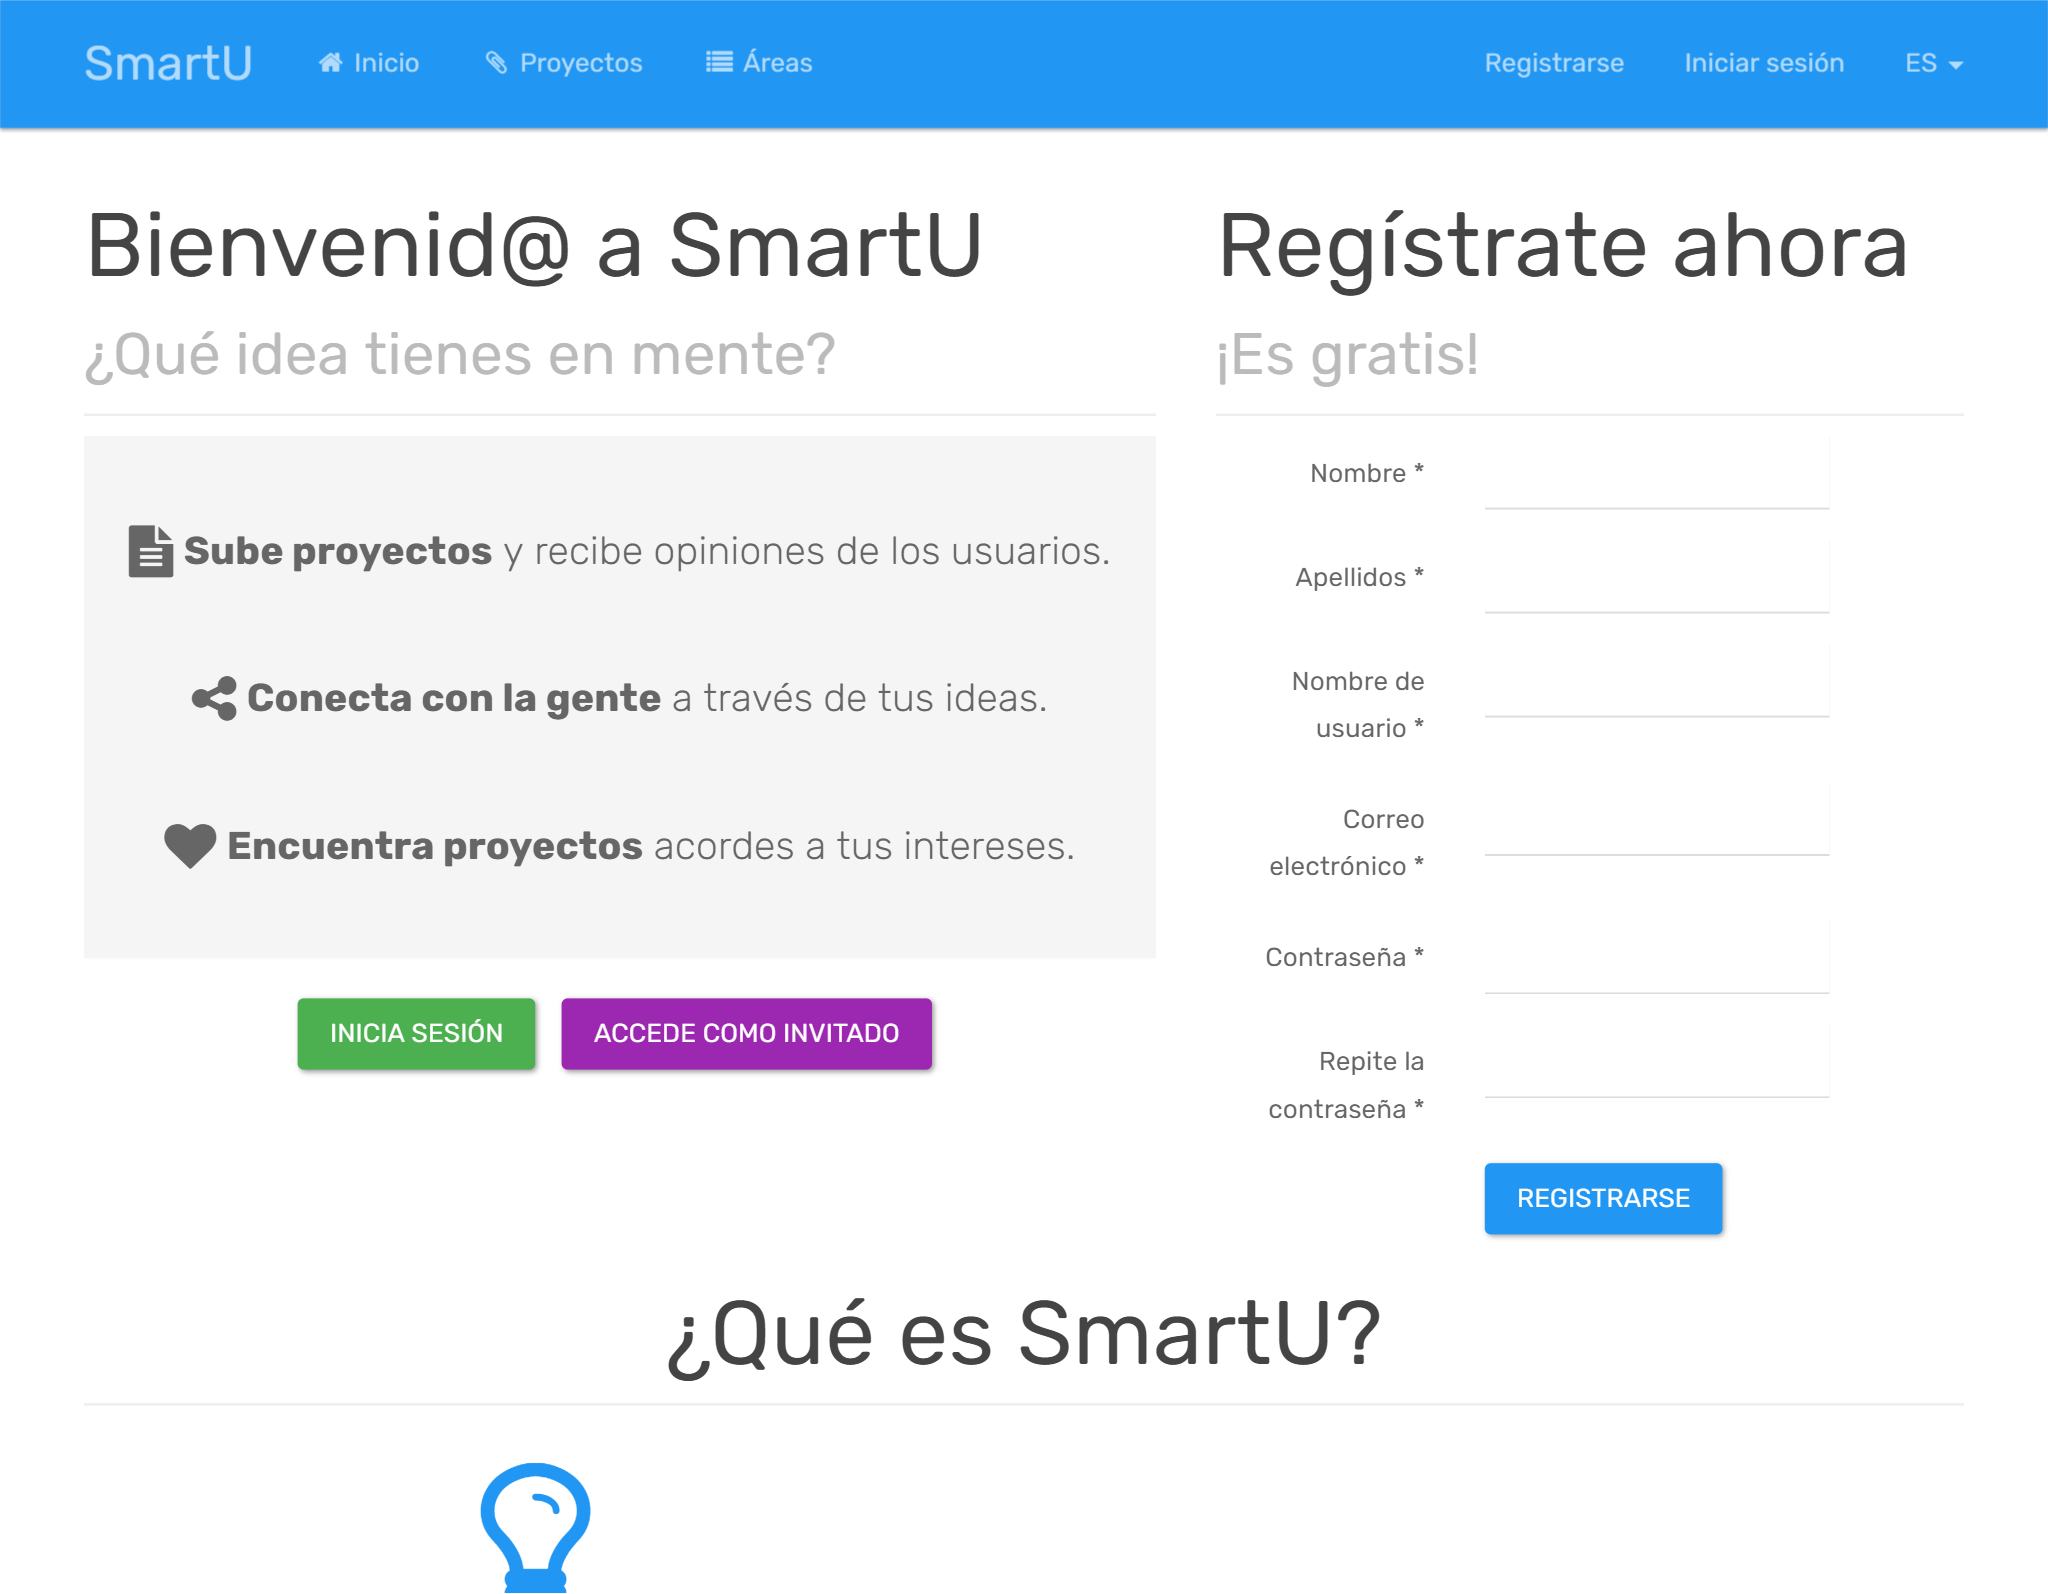
\includegraphics[scale=0.16]{welcome}
    \caption{Página de bienvenida de SmartU}
    \label{welcome}
\end{figure}

\begin{figure}
    \centering
    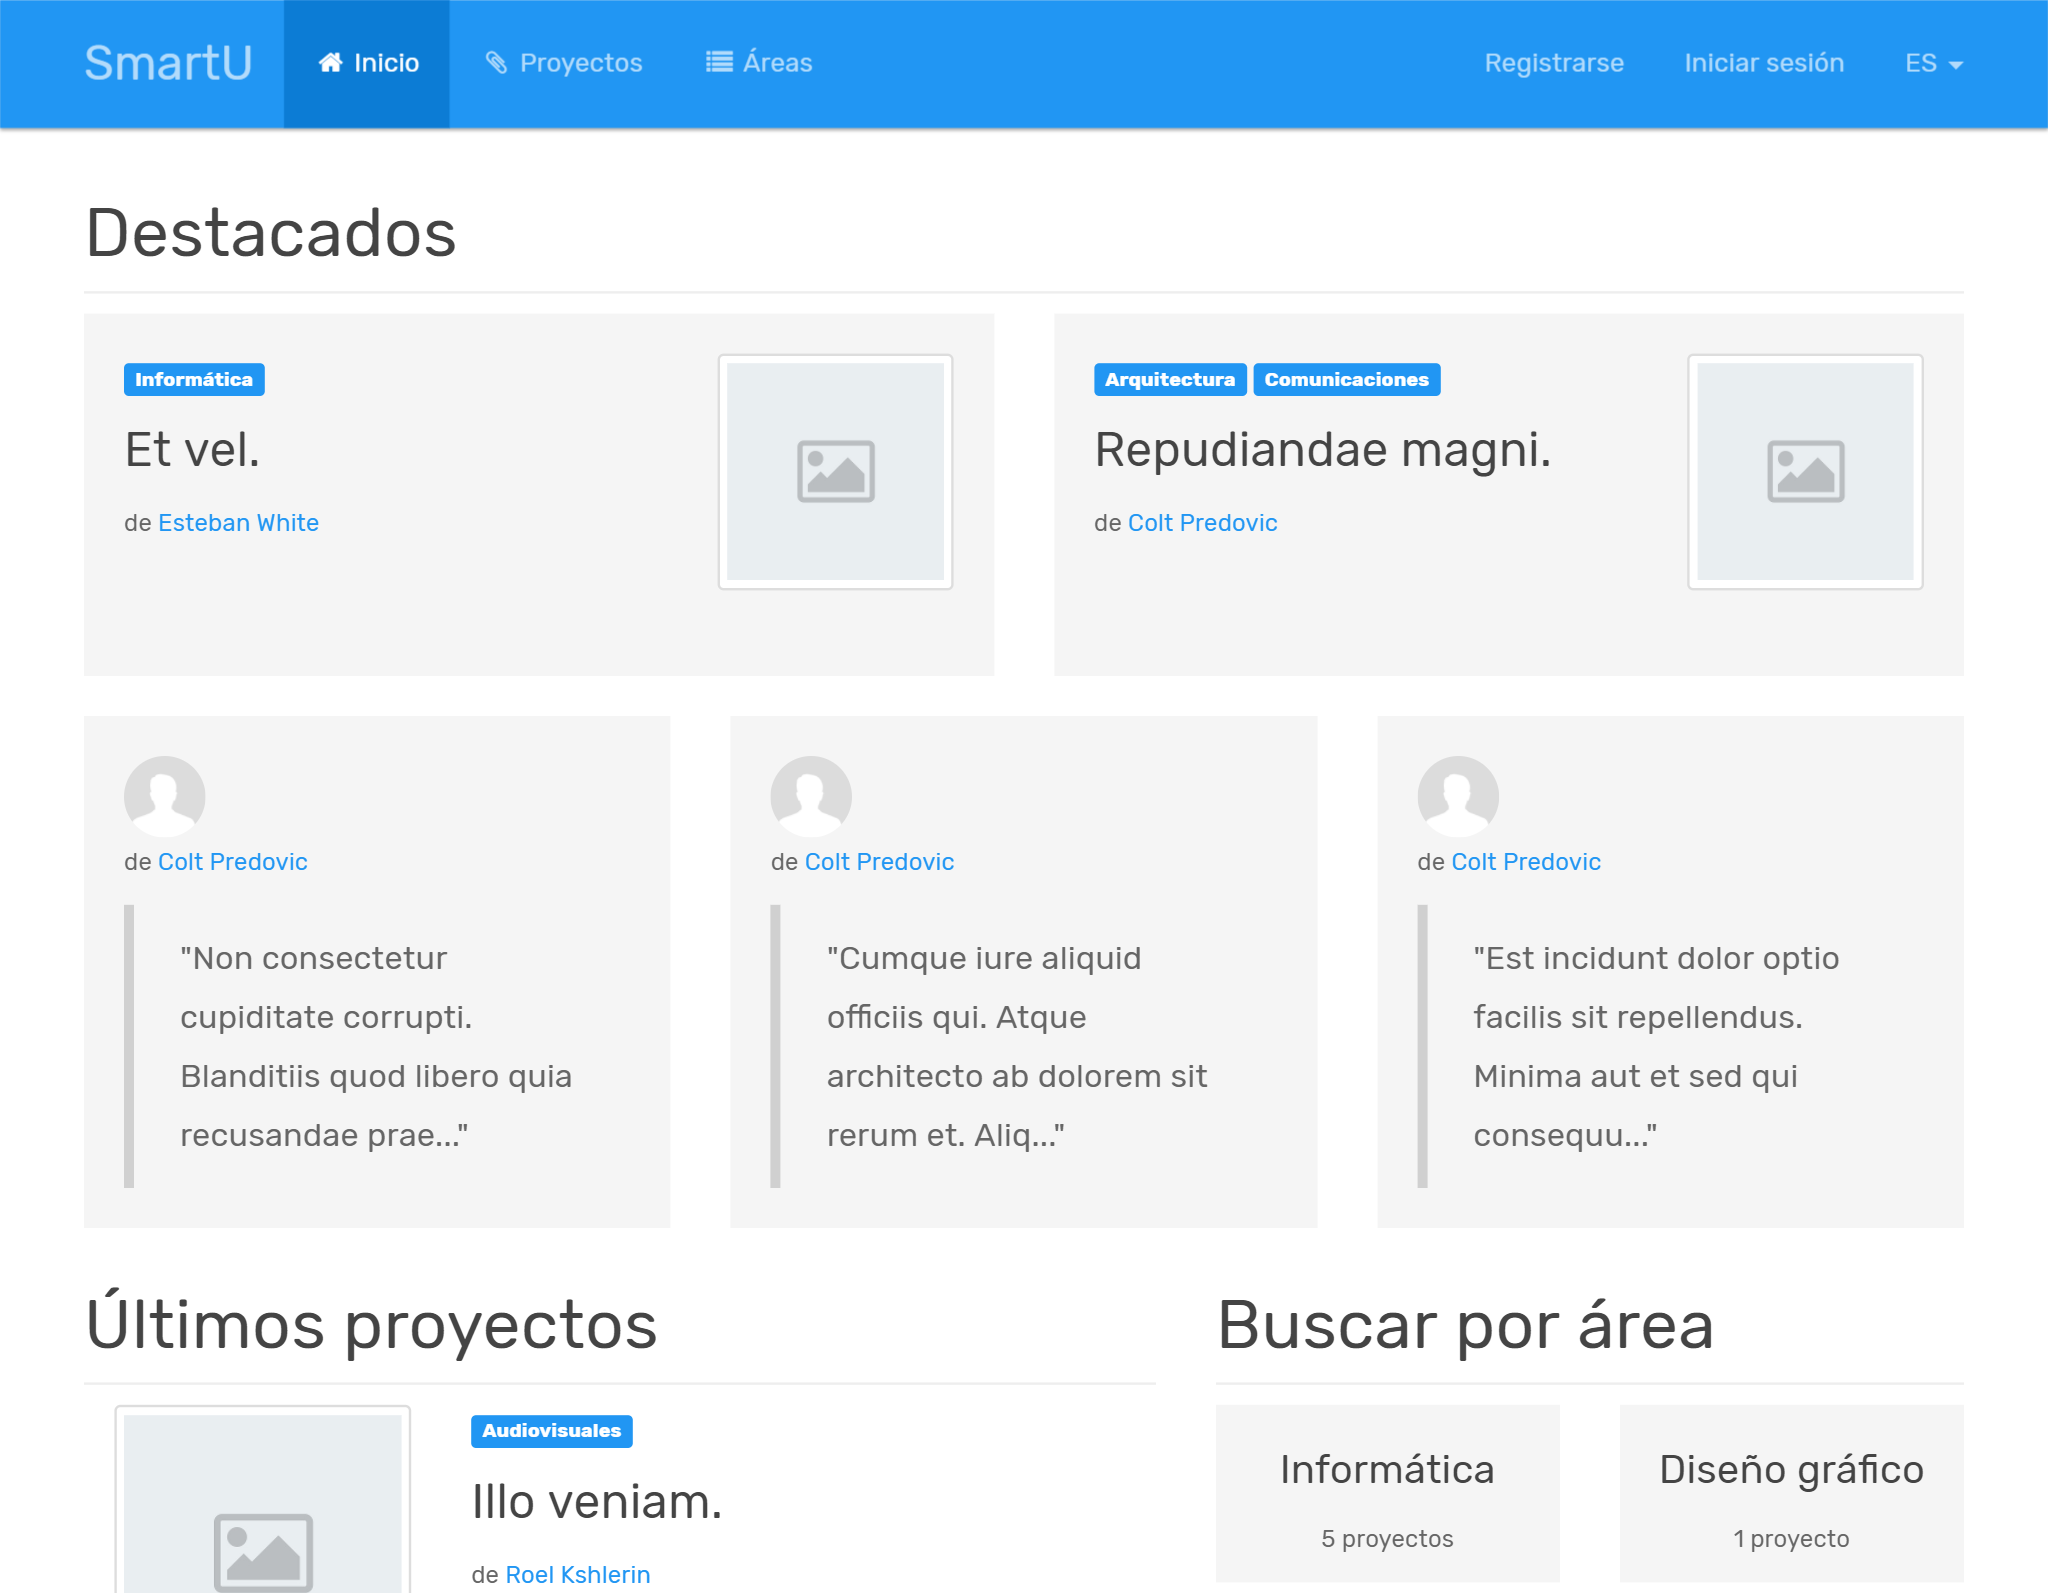
\includegraphics[scale=0.16]{dashboard}
    \caption{Página inicial de SmartU (Destacados)}
    \label{dashboard}
\end{figure}

En la figura \ref{dashboardenglish} se puede apreciar la característica de multilenguaje de la aplicación en la misma página de destacados. Cualquier usuario puede entrar y ver los proyectos, pero para poder interactuar más en SmartU, como por ejemplo dejar un comentario, o publicar un proyecto, nuevo, primero hay que registrarse, tal y como se ve en la imagen \ref{register}.\\

\begin{figure}
    \centering
    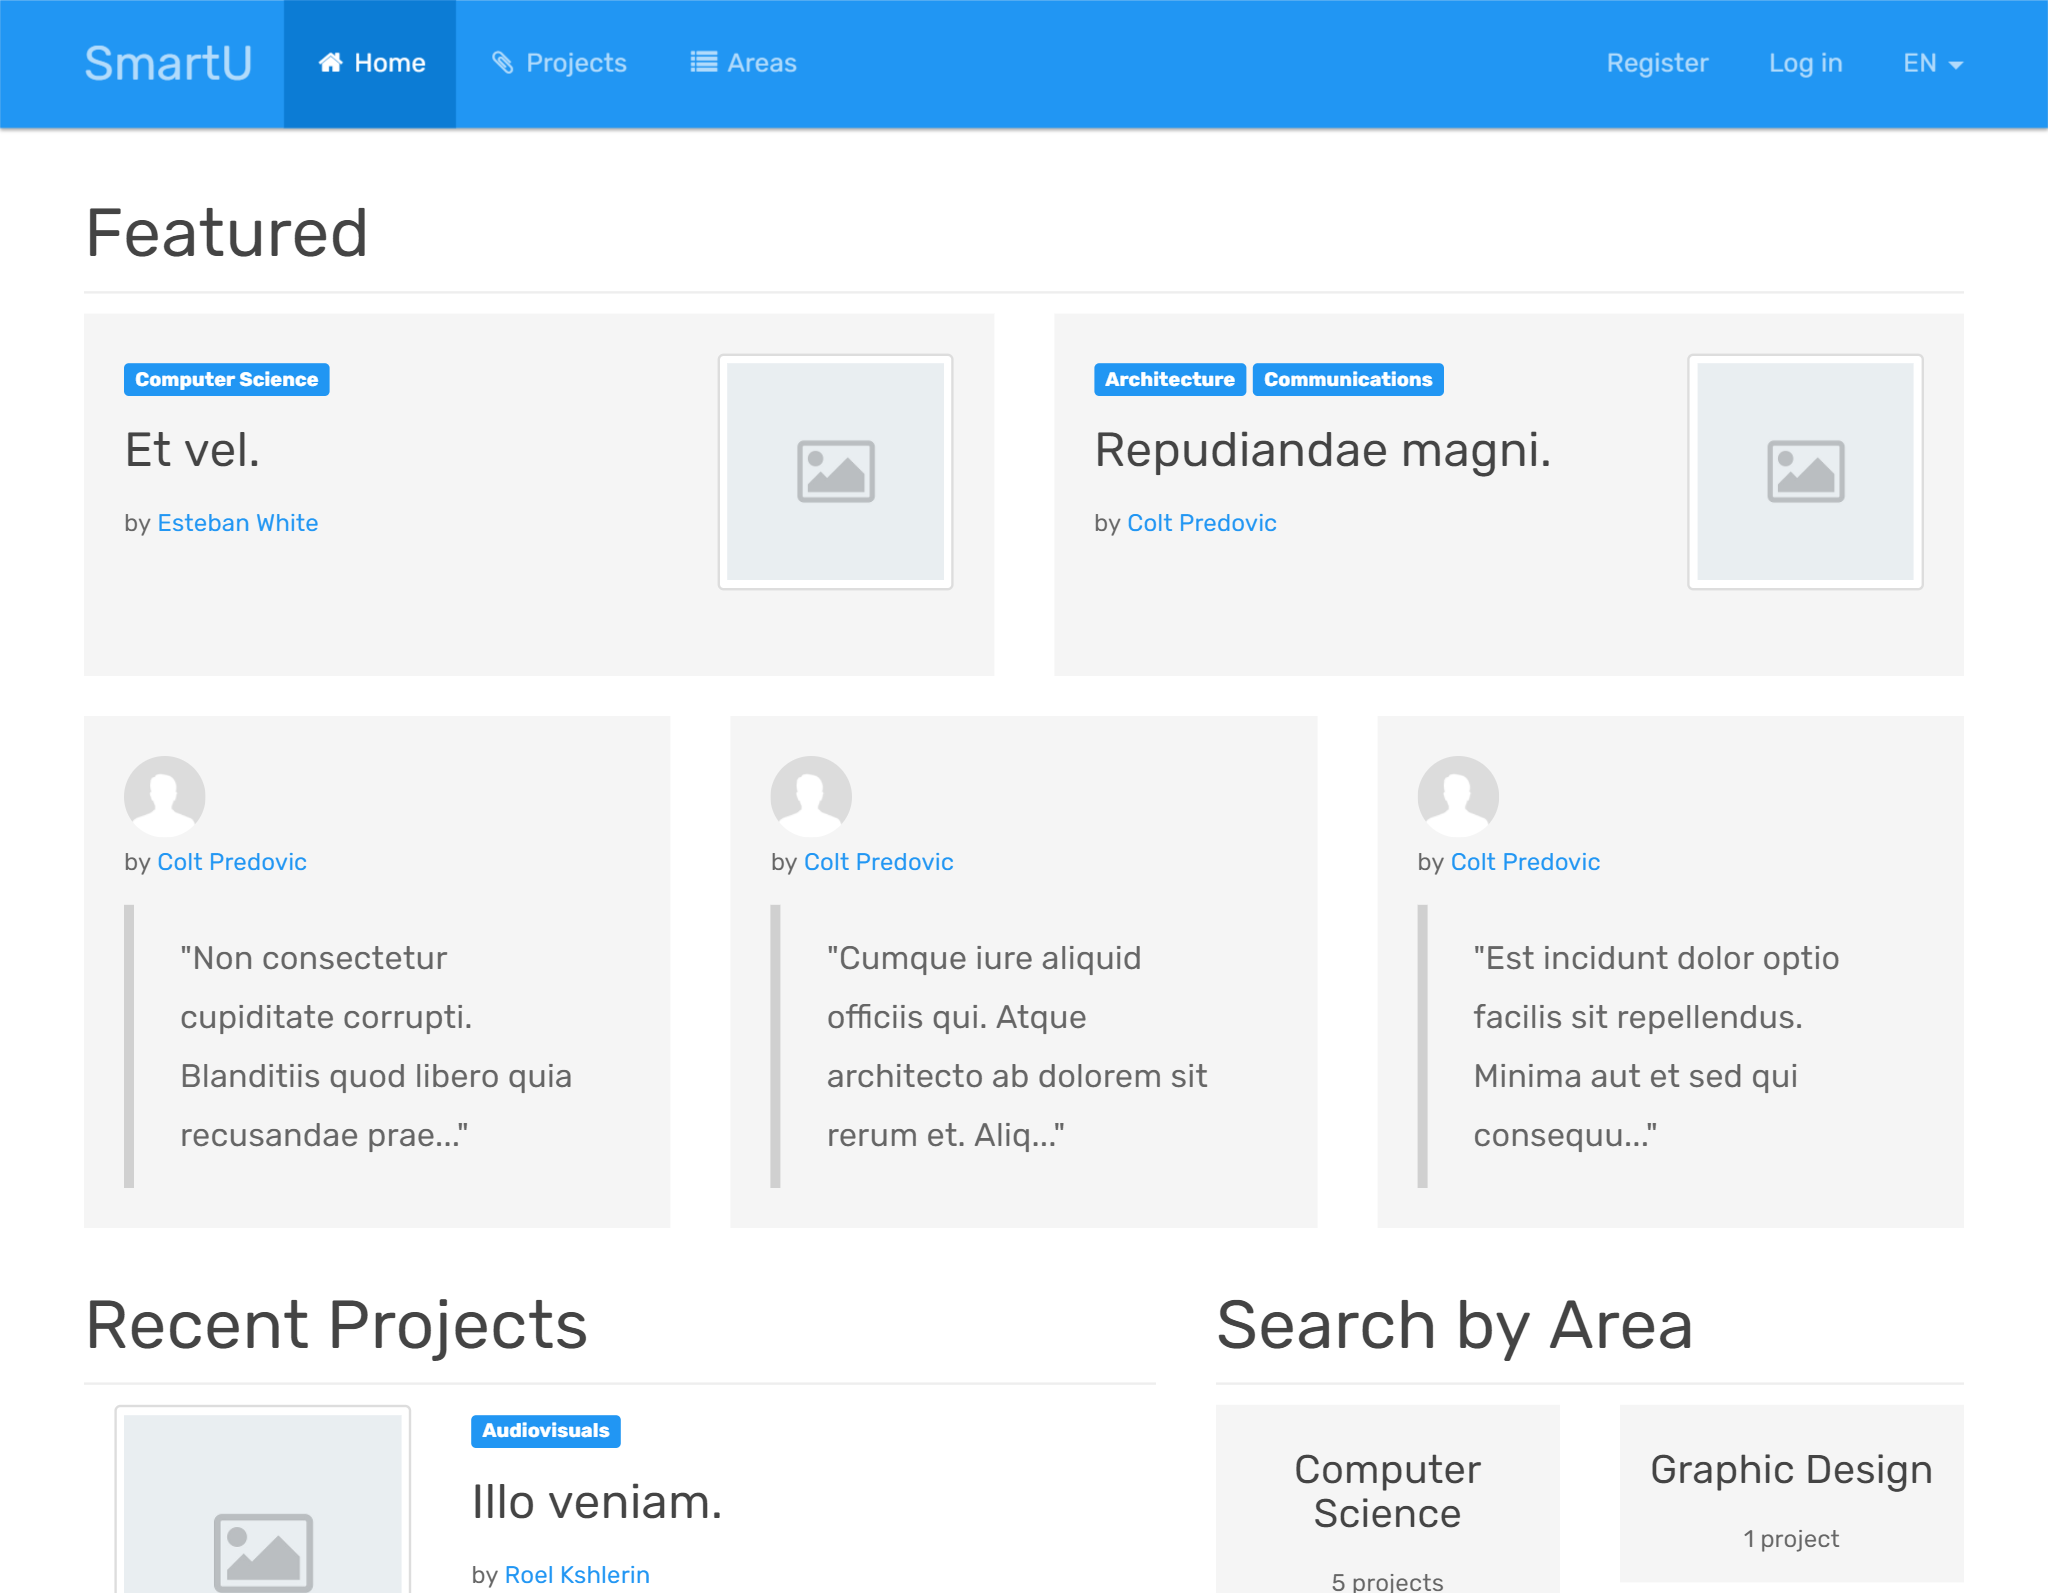
\includegraphics[scale=0.16]{dashboardenglish}
    \caption{Página inicial de SmartU con el idioma en inglés}
    \label{dashboardenglish}
\end{figure}

\begin{figure}
    \centering
    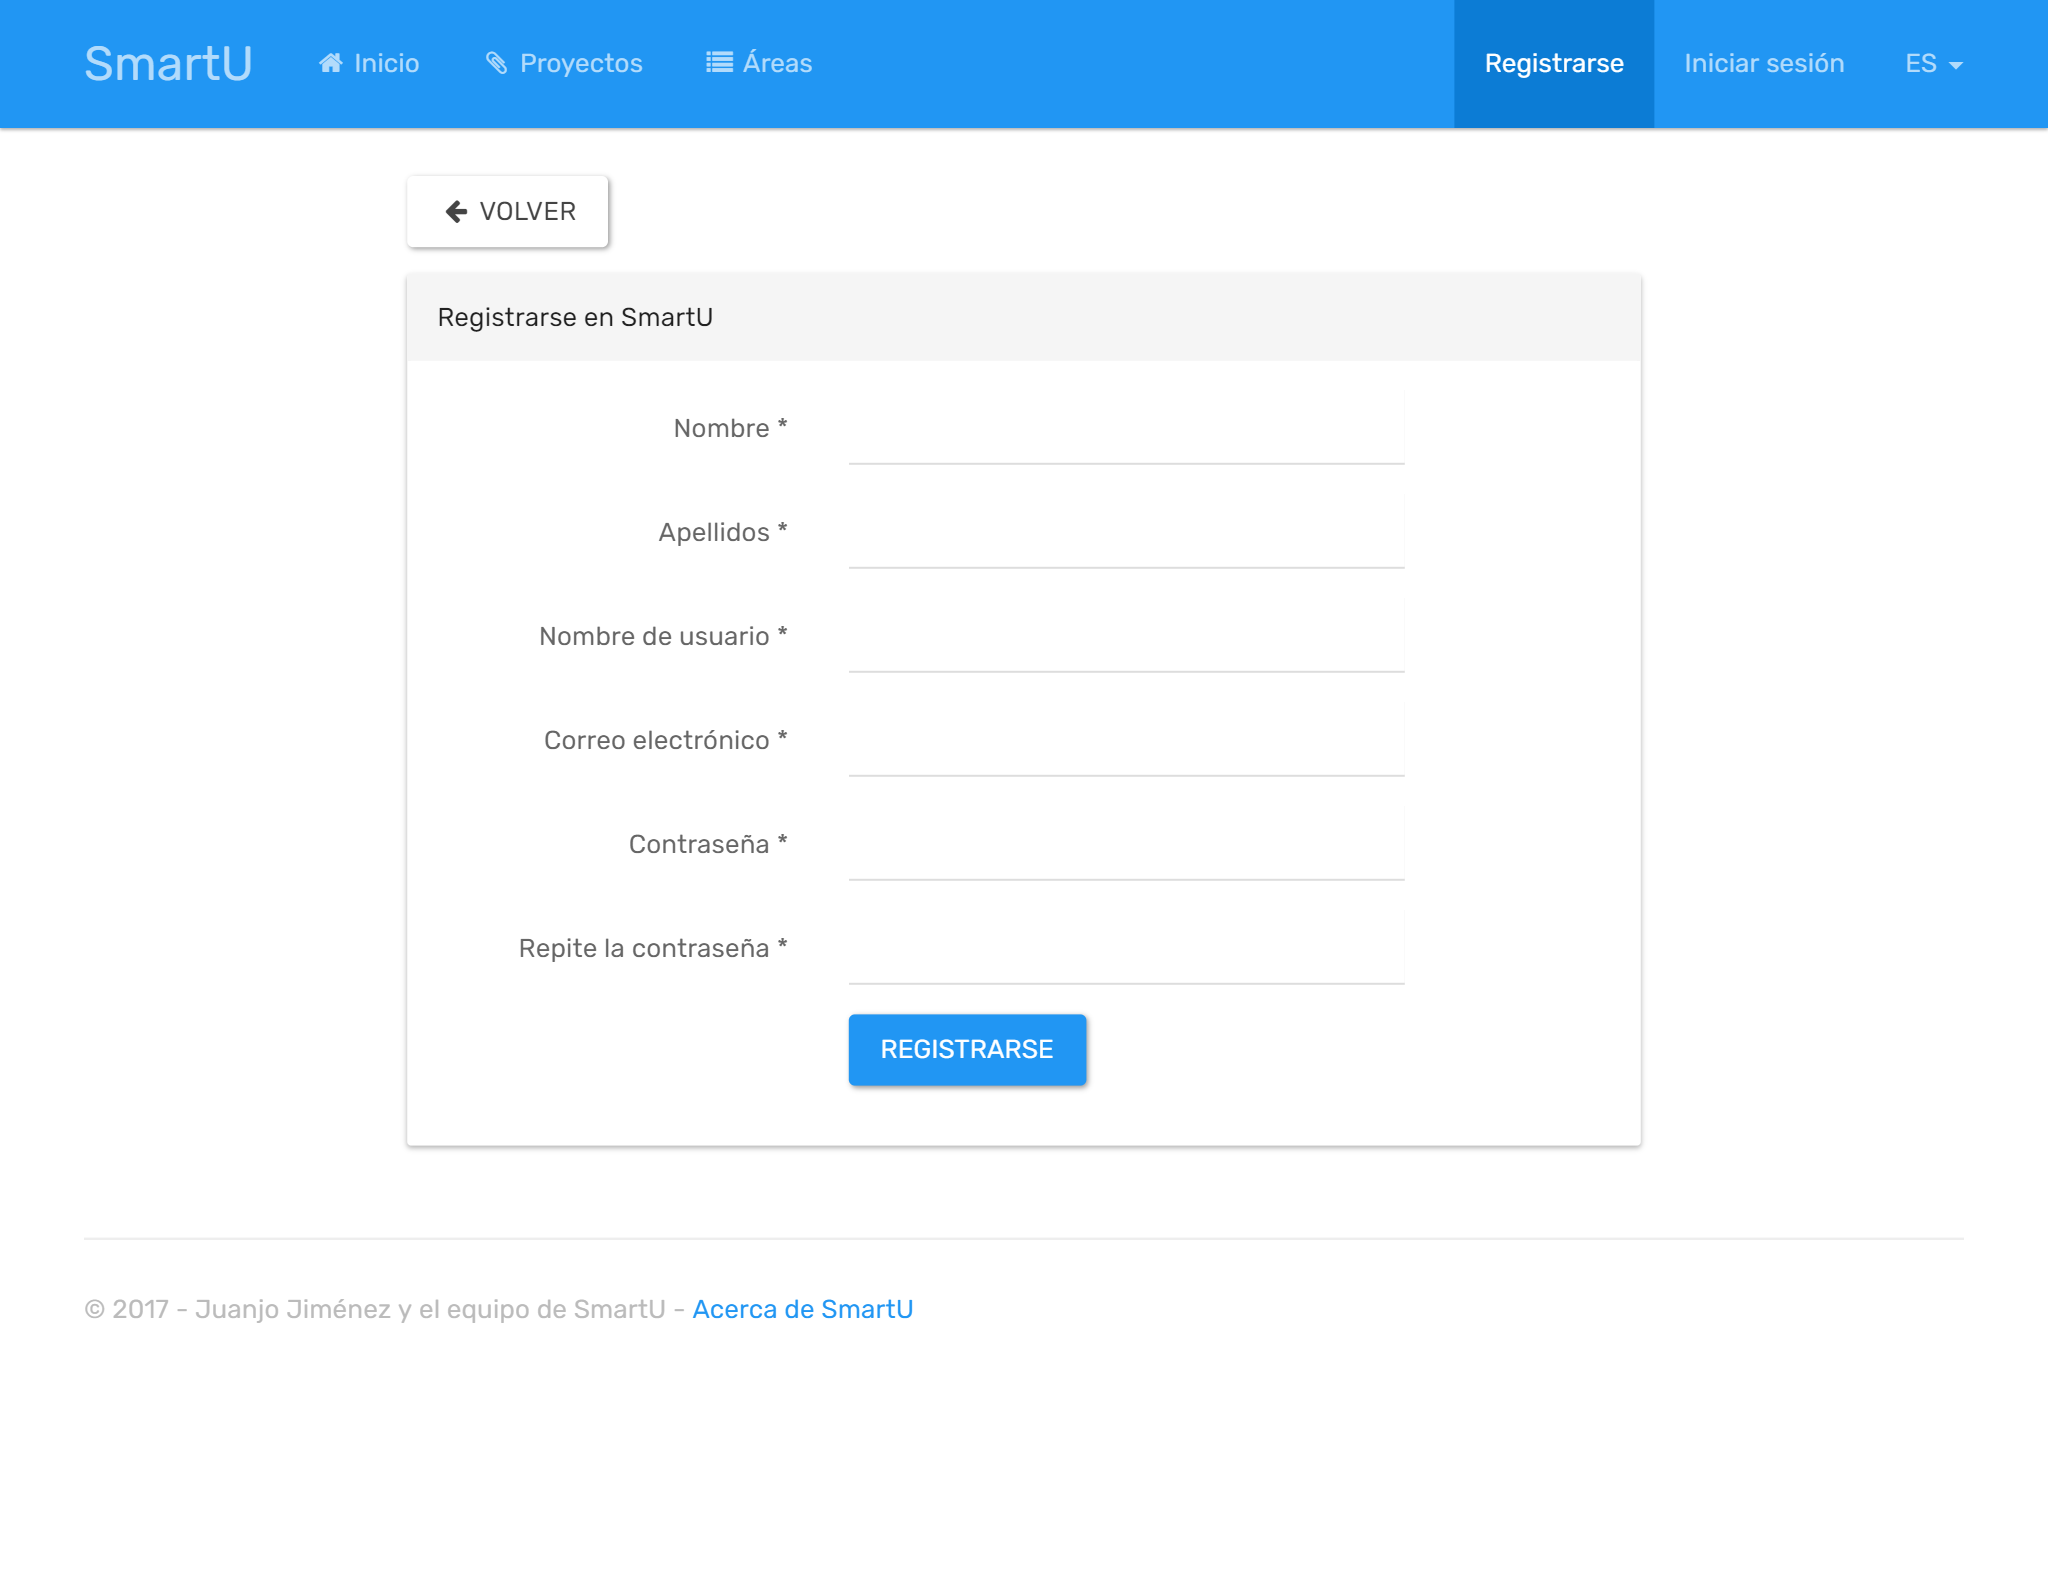
\includegraphics[scale=0.16]{register}
    \caption{Página de registro de un nuevo usuario}
    \label{register}
\end{figure}

En las imágenes \ref{projects}, \ref{project} y \ref{progress} se ve las secciones de \textit{Todos los proyectos}, \textit{Detalle de un proyecto} y la sección de avances (hitos, progresos que se hacen en el proyecto), así como los comentarios que otros usuarios han dejado en el proyecto.

\begin{figure}
    \centering
    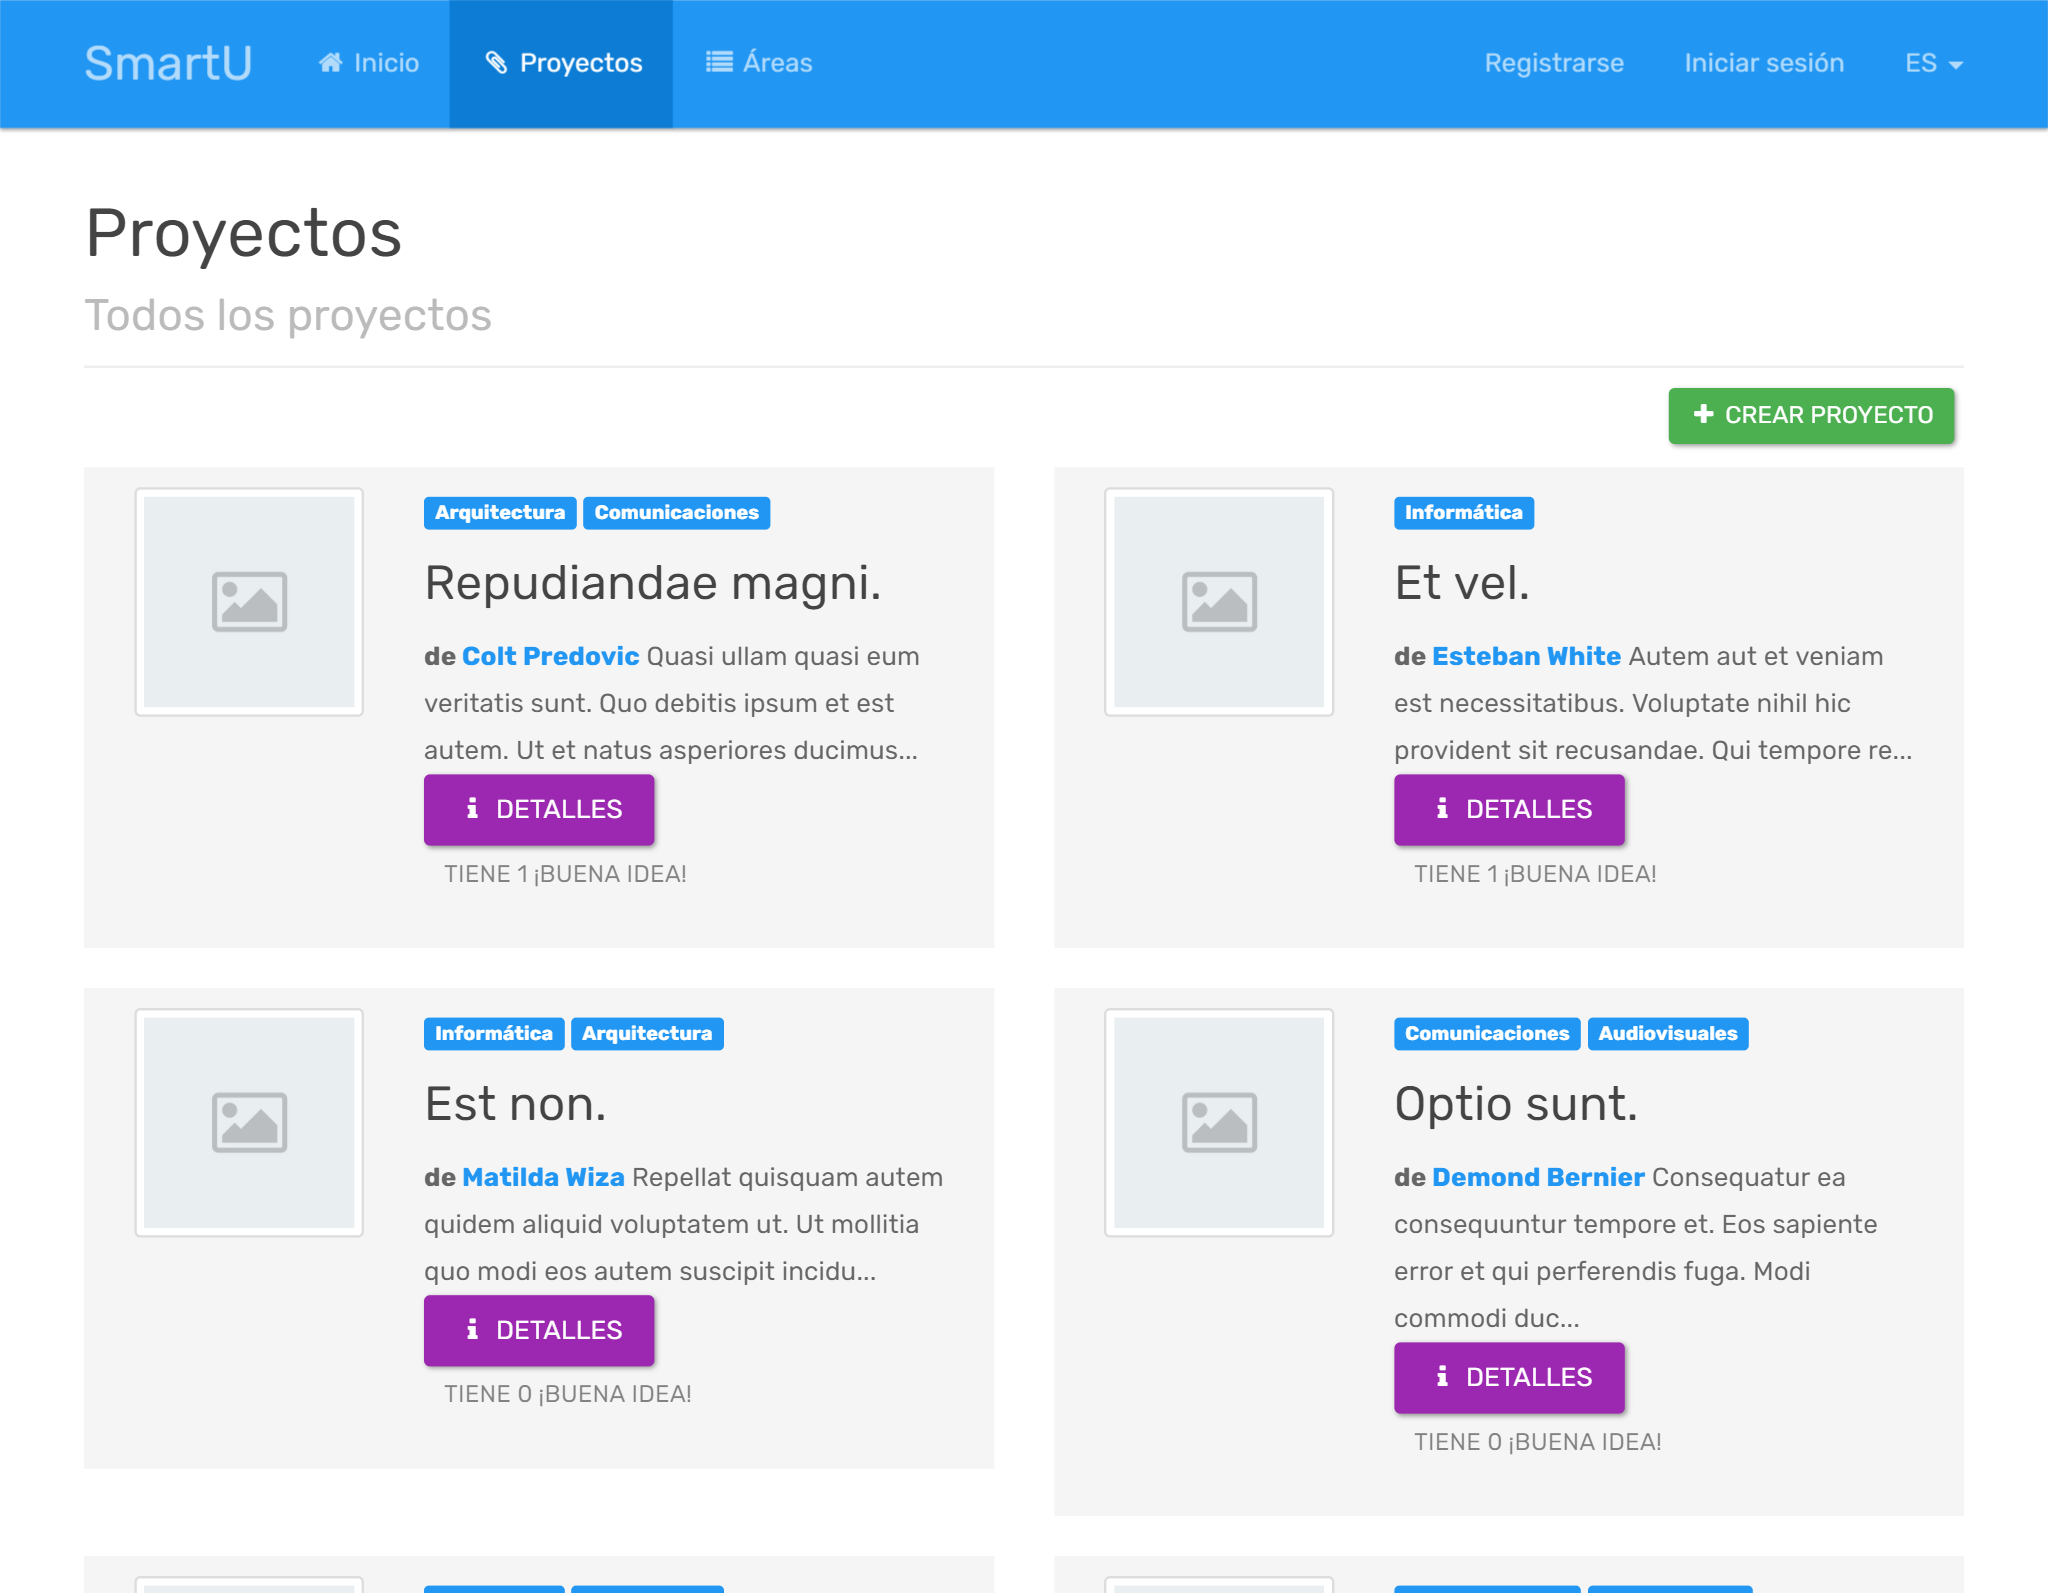
\includegraphics[scale=0.16]{projects}
    \caption{Listado de todos los proyectos}
    \label{projects}
\end{figure}

\begin{figure}
    \centering
    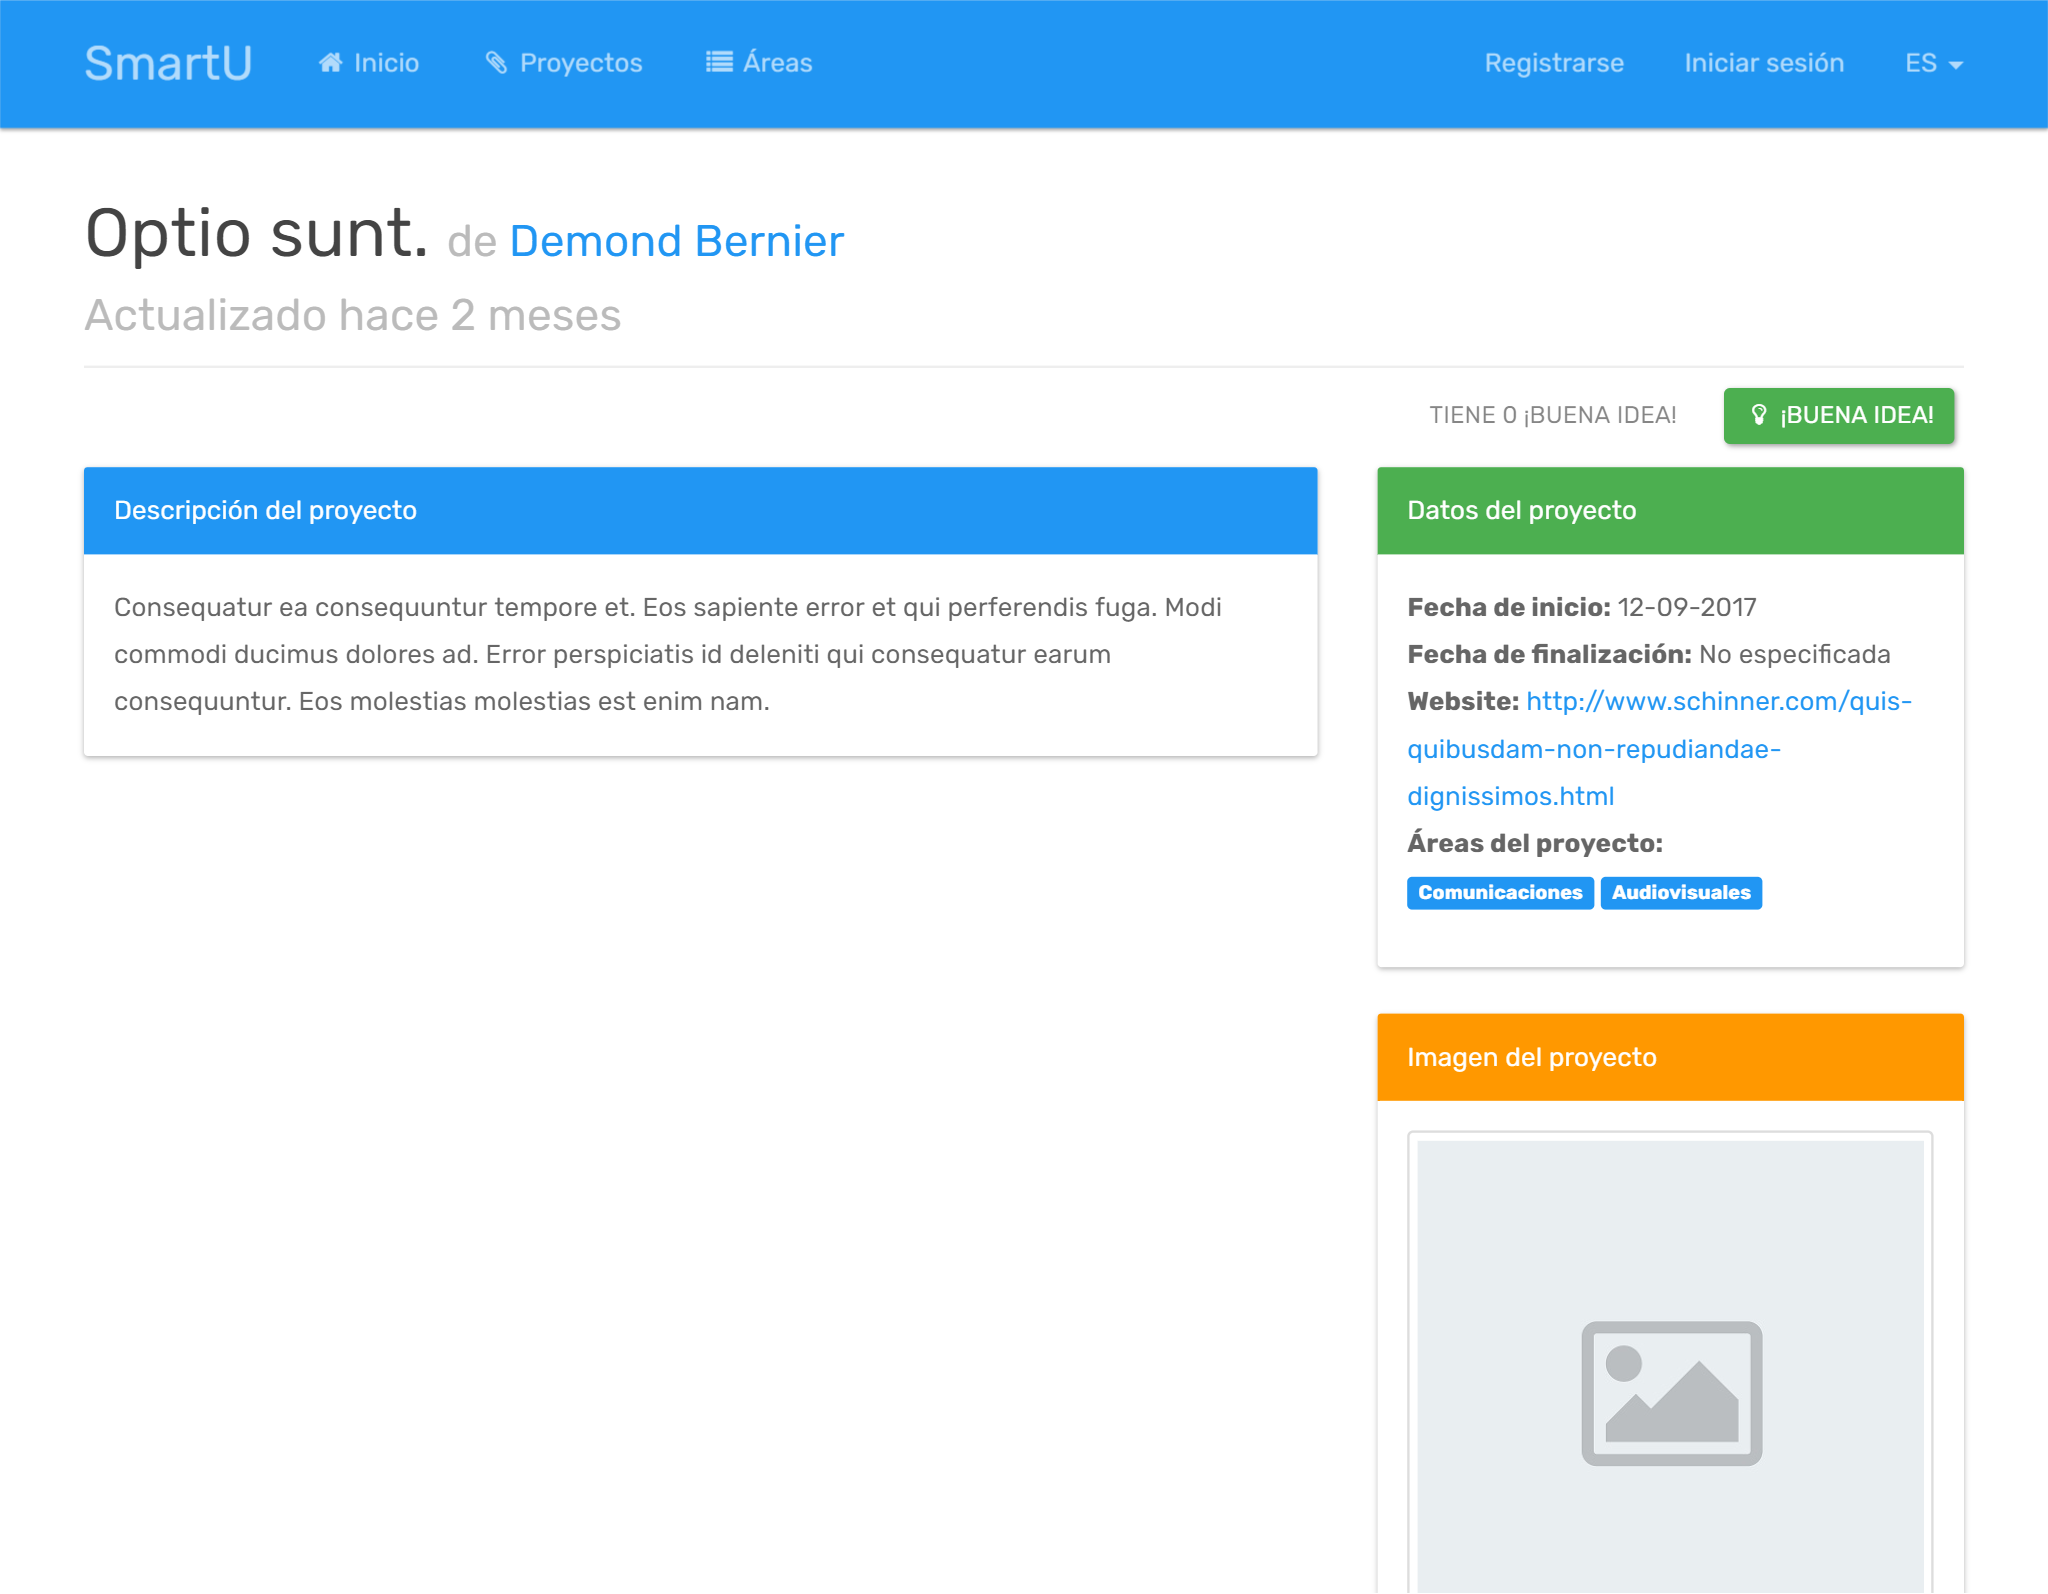
\includegraphics[scale=0.16]{project}
    \caption{Vista de detalles de un proyecto}
    \label{project}
\end{figure}

\begin{figure}
    \centering
    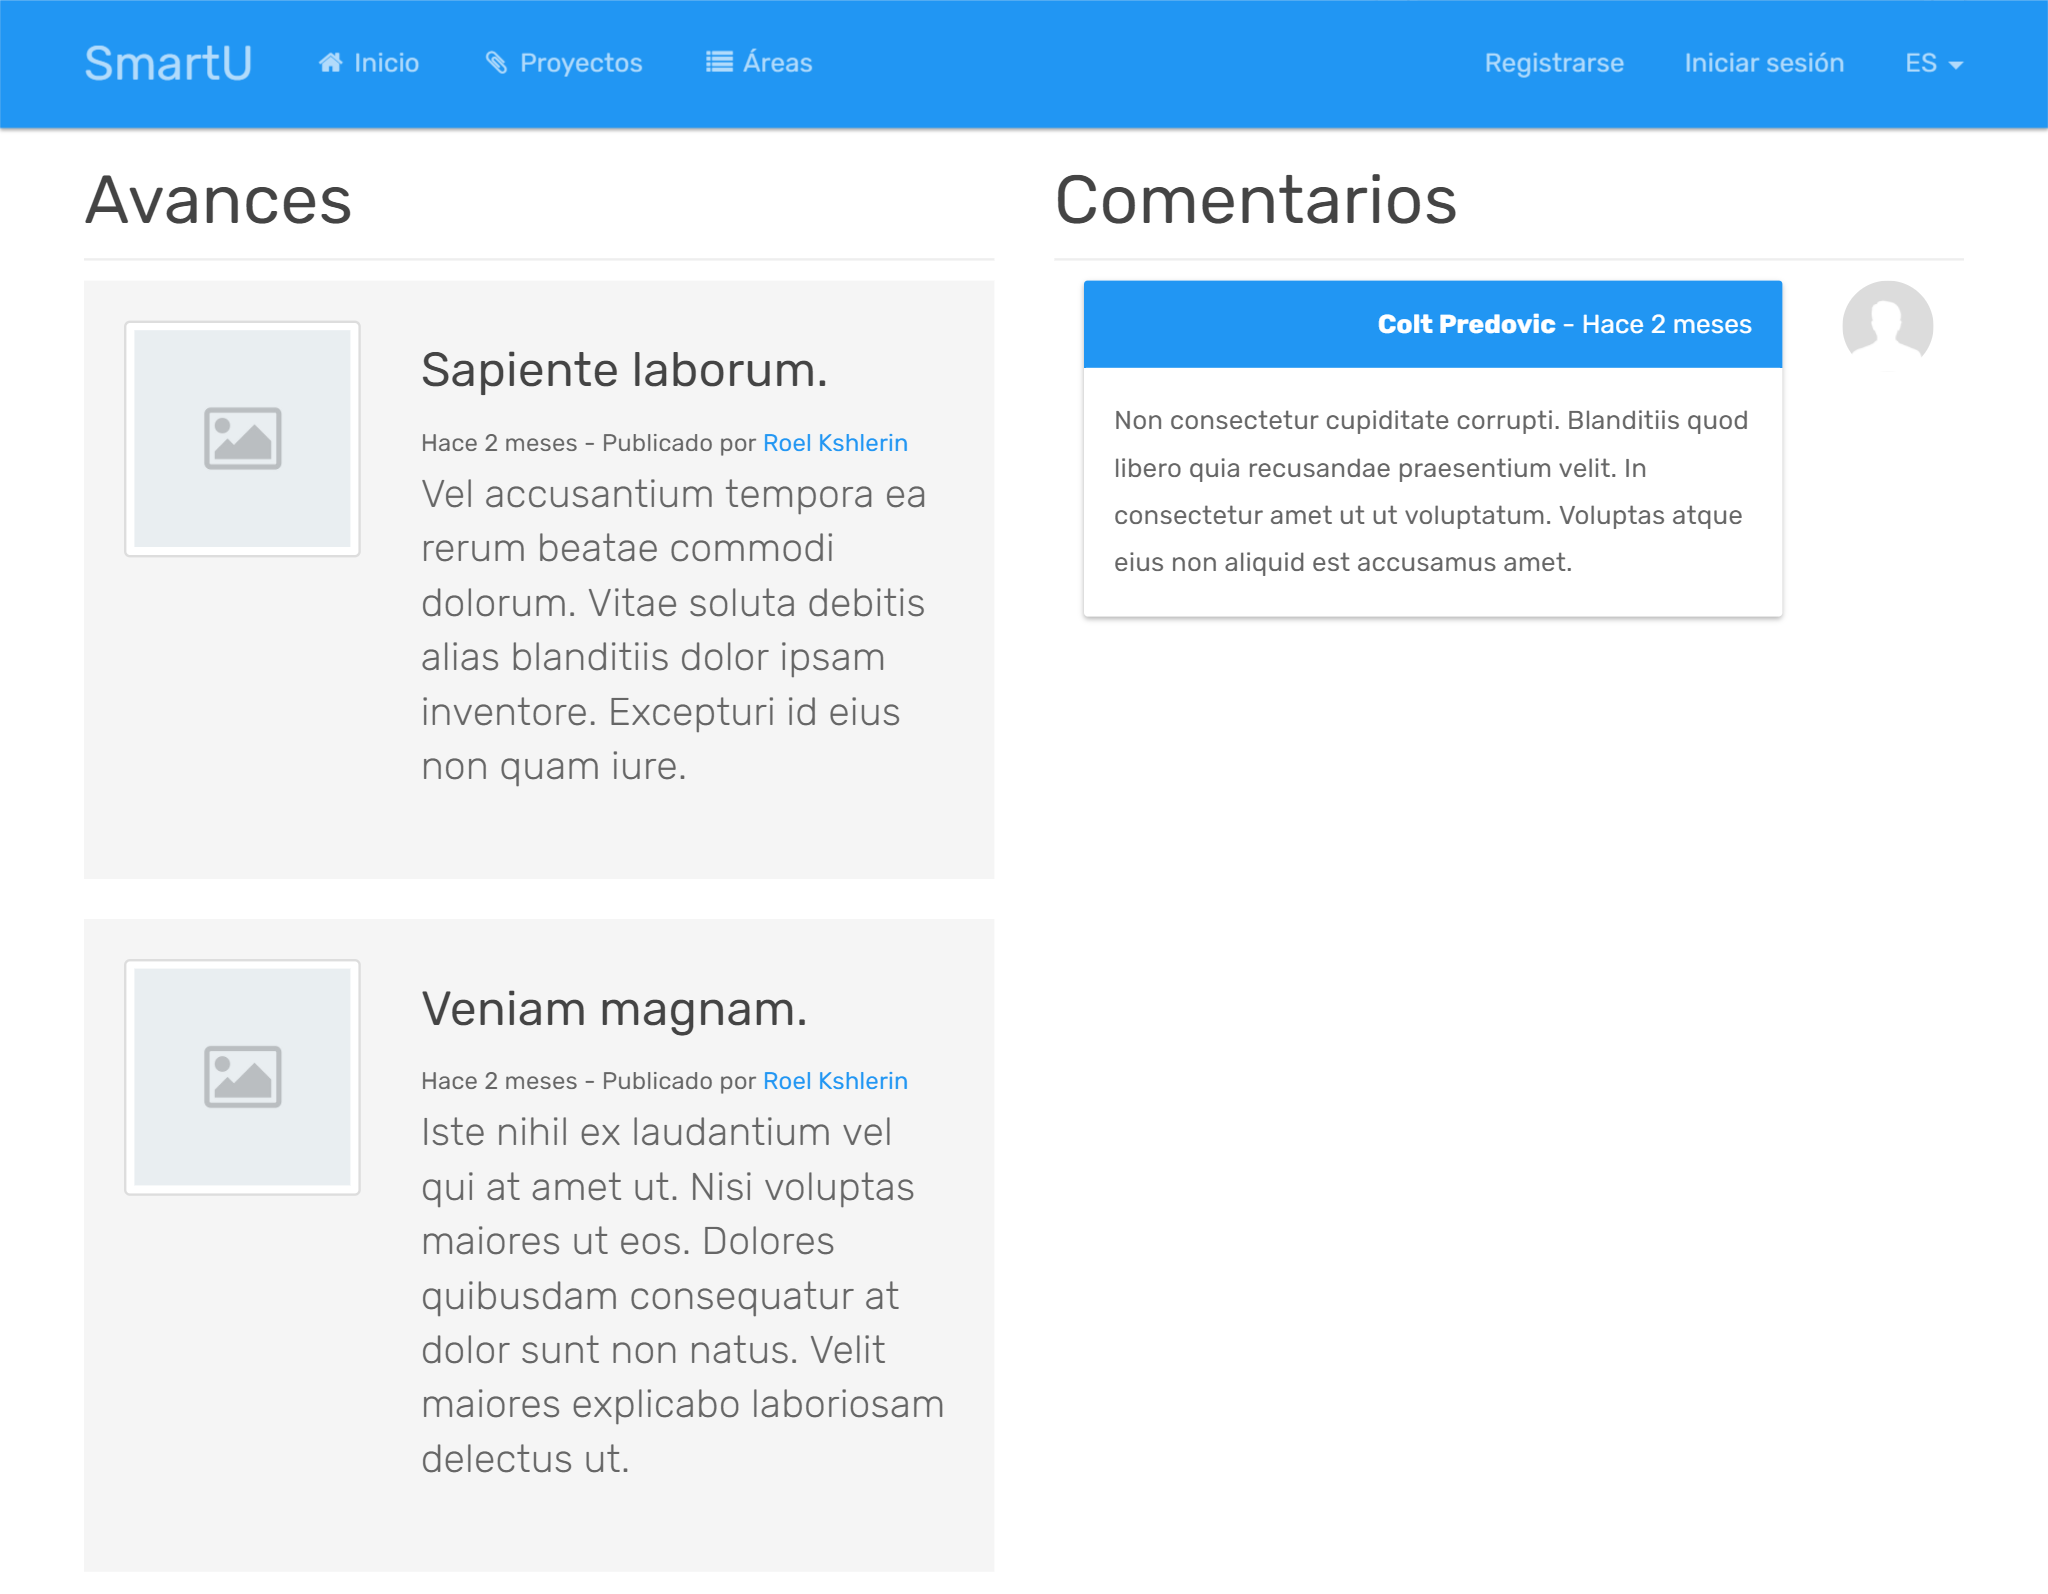
\includegraphics[scale=0.16]{progress}
    \caption{Vista de avances y comentarios de un proyecto}
    \label{progress}
\end{figure}

\chapter{Resultados y Conclusiones}
\label{ch:conclusiones}
Este capítulo recoge los resultados obtenidos de la realización del proyecto, siguiendo las directrices y procedimientos marcados en el capítulo \ref{ch:metodologia}. En este capítulo, se describirán los resultados siguiendo los mismos epígrafes que el capítulo \ref{ch:metodologia}, para así ver de forma más clara cómo ha progresado cada parte de la metodología.\\

Tras el análisis de la misma y una serie de conclusiones positivas y negativas del proyecto, se prosigue con una serie de propuestas de mejora de cara a sucesivas iteraciones del proyecto.

\section{Desarrollo de la metodología}
\subsection{El equipo}
A lo largo del proyecto, el equipo se ha visto afectado por numerosos cambios repentinos y no previstos, que incluyen bajas e incorporaciones de nuevos miembros. Esto requería un esfuerzo adicional de adaptación del nuevo compañero o compañera, al que había que poner en situación del proyecto, conocer sus cualidades y puntos fuertes, etc.\\

En la imagen \ref{asistencias} se puede ver un gráfico de número de asistencias de los miembros del equipo a las reuniones. Ha de tenerse en cuenta que no todos los miebros del equipo entraron al principio.\\

\begin{figure}
    \centering
    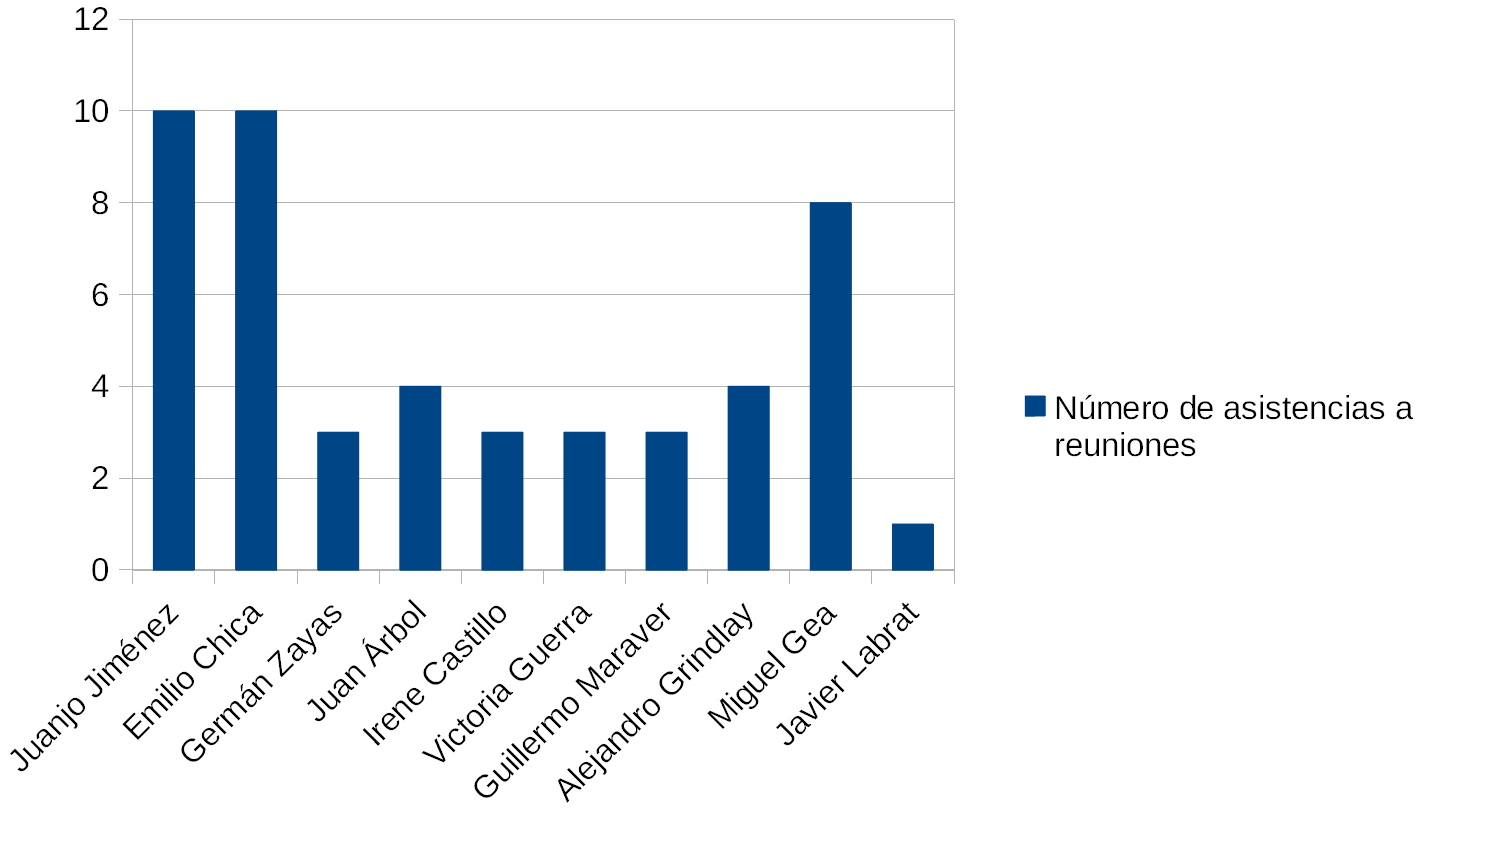
\includegraphics[scale=0.8]{asistencias}
    \caption{Gráfico de asistencias de los integrantes a las reuniones}
    \label{asistencias}
\end{figure}

Debido a la amplia disparidad de tiempo disponible que tenía cada uno de los integrantes, la coordinación no fue del todo exitosa. Surgieron numerosos contratiempos de planificación de reuniones. Esto afectó en cierta medida a la temporización del proyecto, que se ve con más detalle en el siguiente apartado.\\

Para lograr una mejor coordinación, este tipo de proyectos requieren de más dedicación y coordinación. Se ha visto que acciones como encontrar un día de la semana común para organizar reuniones semanales ayuda en gran medida a la organización. En caso de que no pueda asistir alguien en alguna ocasión a las reuniones, las actas de reunión son una buena forma de que los ausentes se pongan al día en lo que se ha avanzado.\\

Durante el proyecto, se realizaron una serie de actas más básicas que recogían lo esencial que fue tratado en la reunión, pero en el anexo se puede encontrar una propuesta de plantilla más elaborada que permite organizar y controlar mejor los asuntos del proyecto, como las tareas planificadas, objetivos para siguientes reuniones, etc.

\subsection{Temporización}
La planificación inicial que se realizó sufrió grandes variaciones a lo largo del curso. Debido a varios retrasos y dificultades para la organización de las reuniones, se sufrían retrasos de varias semanas hasta poder encontrar puntos comunes en los que la mayoría de personas del equipo se podían reunir. En la tabla \ref{temporizacion} se puede consultar la temporización del proyecto.\\

\begin{table}
    \begin{center}
        \begin{tabular}{|p{5cm}|p{3cm}|p{3cm}|}
            \hline
                \rowcolor{Gray}\multicolumn{1}{|c|}{\textbf{Hito o tarea}}
                & \multicolumn{1}{|c|}{\textbf{Fecha de inicio}}
                & \multicolumn{1}{|c|}{\textbf{Fecha de finalización}}\\
            \hline
                Reuniones iniciales de presentación, explicación y creación de seminarios & Principios de noviembre de 2016 & Finales de diciembre de 2016 \\
            \hline
                Creación de seminarios y design thinking & Principios de febrero de 2017 & Finales de marzo de 2017\\
            \hline
                Realización de los seminarios de tecnologías y Design Thinking & Finales de marzo de 2017 & Principios de abril de 2017 \\
            \hline
                Comienzo del desarrollo del proyecto y tareas asignadas a cada miembro & Principios de mayo de 2017 & Principios de junio de 2017 \\
            \hline
                Reuniones finales de testeo y coordinación de defensas de TFGs & Principios de junio de 2017 & Mediados de junio de 2017 \\
            \hline
                Finalización de la documentación de mi proyecto & Principios de julio de 2017 & Finales de noviembre de 2017 \\
            \hline
        \end{tabular}
        \caption{Temporización general del proyecto}
        \label{temporizacion}
    \end{center}
\end{table}

\subsection{Seminarios y divulgación}
Una vez expuesto el catálogo de posibles técnicas de creatividad y generación de ideas, se optó por realizar un \textbf{seminario informativo de tecnologías emergentes}, otro sobre \textbf{técnicas de creatividad}, seguido de un proceso creativo de \textit{Design Thinking} para que todos aportaran ideas y conceptos que nos servirían para dar forma a nuestro sistema a desarrollar. En el anexo \ref{sec:designthinking} podrá encontrar una \textbf{lista de todas las ideas} que se obtuvieron, clasificadas de la siguiente manera:

\begin{itemize}
    \item Ideas
    \item Objetivos
    \item Limitaciones
    \item Aspectos positivos
\end{itemize}

Más adelante se realizó otra sesión de Design Thinking debido a que hubo algunas ausencias en la primera reunión, y sirvió para \textbf{afianzar todo lo visto} en la primera y proceder con ello al desarrollo del producto software, que se detalla en el capítulo \ref{ch:desarrollo}.\\

En el anexo puede encontrar disponible las actas de reunión realizadas durante este primer año de vida del proyecto.

\subsection{Comunicación}
Como detalle final de la gestión de la comunicación, en la tabla \ref{canalescomunicacion} se puede ver las valoraciones dadas tras su uso a los distintos canales de comunicación que utilizamos entre los miembros del equipo.

\begin{table}
    \begin{center}
        \begin{tabular}{|l|p{3cm}|p{5cm}|}
            \hline
                \rowcolor{Gray}\multicolumn{1}{|c|}{\textbf{Canal}}
                & \multicolumn{1}{|c|}{\textbf{Utilidad}} & \multicolumn{1}{|c|}{\textbf{Valoración}} \\
            \hline
                E-mail & Usado en las primeras semanas & No es recomendable, debido a que no siempre se comprueba el correo electrónico con regularidad y no se sabe si alguien lo ha leido. \\
            \hline
                WhatsApp \cite{whatsapp} & Utilizado durante todo el proyecto & Aplicación de mensajería más utilizada, respuesta casi inmediata y mayor rapidez de comunicación. \\
            \hline
                Slack \cite{slack} & Utilizado al final del proyecto & Es una plataforma muy utilizada por empresas y equipos de desarrollo, con numerosas funcionalidades de comunicación entre miembros que agilizan bastante la comunicación. \\
            \hline
        \end{tabular}

        \caption{Canales de comunicación empleados y valoración de los mismos}
        \label{canalescomunicacion}
    \end{center}
\end{table}

A pesar de las ventajas que aportaba Slack, finalmente no se utilizó de forma global en el equipo, sino únicamente por un grupo reducido de personas del mismo. El motivo es que requiere de una pequeña introducción al resto de compañeros para que conozcan los fundamentos básicos de su funcionamiento, pero no se realizó dicha clase introductoria.\\

A pesar de esto, se recomienda el uso de Slack y para ello, se sugiere que al empezar un nuevo proyecto, una de las primeras tareas sea la de enseñar a usarlo y fomentarlo.

\subsection{Dependencias entre miembros del equipo}
Nos encontramos con los siguientes ejemplos de tareas en las que hemos encontrado sinergias, es decir, que gracias a la colaboración mutua, el resultado obtenido es mejor que haberlo hecho por separado:

\begin{itemize}
    \item La propia \textbf{implementación de las plataformas} colaborando con mi compañero Emilio consiguió que el software propuesto presentara una funcionalidad más rica y completa que haberlo hecho por separado.
    \item Germán aportó sinergias en casi todas las líneas de trabajo, ya que su tarea (\textbf{diseño de la identidad corporativa}) es aplicable no solo al software, sino también al marketing.
    \item Entre Germán y Juan hubo colaboración para confeccionar el diseño de la \textbf{página web de presentación del proyecto}, así como la creación de sus contenidos.
    \item Javier, con su proyecto ya terminado, sirvió como \textbf{prueba de concepto}, al permitir incorporar su proyecto al futuro sistema que se va a diseñar para demostrar al público objetivo las capacidades de SmartU.
\end{itemize}

Pero también es cierto que hubo ciertos problemas a lo largo del curso que impidieron la aprición de más sinergias. Principalmente los problemas fueron la falta de tiempo para que algunos miembros pudieran hacer sus tareas, y la tardía definición de todos los conceptos del proyecto y la necesidad de la aplicación móvil, que en un principio no quedaba clara cual podía ser tu utilidad y diferenciación.\\

Esta experiencia nos hace ver que este tipo de proyectos requieren de más dedicación de la que se pensaba. Al ser una primera experiencia piloto, no teníamos del todo claro lo que podía pasar, pero ello nos servirá para que en los años siguientes el proceso mejore.

\section{Valoración personal}
Tras todos estos meses de trabajo, la experiencia adquirida es de enorme valor. Aunque ha habido contratiempos, no se puede negar que se han hecho importantes progresos en el inicio de este proyecto. Se ha conseguido formar un equipo de trabajo de diferentes especialidades y se ha podido obtener de todos ellos mucha información, además de aprender a aprovechar los puntos fuertes de cada uno para realizar partes de este proyecto.\\

Personalmente, quiero destacar que ha sido muy revelador el haber compartido trabajo con personas de otras disciplinas y estudios. Tras muchos años trabajando en equipo con compañeros informáticos, nos acostumbramos demasiado y no sabemos tratar con personas que no tienen los mismos conocimientos que nosotros. Junto a esto, ha sido positivo el haber podido coordinar en la medida de lo posible a todos para poder reunirnos sin alterar la rutina y obligaciones diarias de cada uno de los miembros.\\

El trabajo en equipo nunca es fácil, ya que requiere de un gran compromiso por parte de todos los integrantes para que pueda haber un cierto nivel de éxito. No importa que sea poco al principio si se consigue poner la primera piedra de un proyecto que se espera que a largo plazo se refine más. El hecho de poder coordinar (en mayor o menor medida) a estudiantes de diferentes disciplinas de conocimiento pone en valor lo enriquecedor que supone un trabajo que recibe apoyo de distintos puntos de vista.\\

Por ello, espero que estas páginas y las de los proyectos del resto de mis compañeros sean en el futuro de gran utilidad y permitan que en el futuro, los proyectos multidisciplinares sean una parte más dentro de la vida universitaria, y que los estudiantes no tengan miedo a adentrarse en un proyecto en equipo. Nadie dijo que fuese algo fácil, pero no es imposible.\\

Debido a que la tarea de gestión del proyecto ha sido más laboriosa y ha requerido más tiempo y esfuerzo para llevarla a cabo, por el hecho de organizar y sincronizar a los integrantes del equipo, como consecuencia de ello, mi tarea de desarrollo de software se ha visto mermada y reducida en tiempo y recursos para poder completarla.\\

De esta situación, puedo afirmar que la tarea de gestión alberga una dedicación y complejidad que haría más recomendable que la persona a cargo de la misma, no dedique su tiempo y esfuerzo a otras tareas diferentes, ya que es posible que, o no realice una correcta gestión y atienda a la organización de todos los miembros, o sus otras tareas sean de una calidad reducida.

\section{Objetivos conseguidos}
Aunque el proyecto ha tenido sus problemas, quiero destacar que se han logrado varios objetivos gracias al esfuerzo y trabajo de todos los compañeros. En primer lugar, hemos creado una primera versión de una metodología de trabajo en equipo que confiamos en que mejore con los años. A modo de experimento, hemos aplicado nuestros actuales conocimientos y hemos visto las fortalezas y debilidades de esta forma de trabajar.

\subsection{Productos creados}
Es importante que, como gestor del proyecto, además de desarrollador, ponga en valor todo lo que se ha ido creando, ya que, aun incompletos, existen una serie de \textit{deriverables} que sirven como base para completar en el futuro.\\

\subsubsection{Software}
Tenemos las primeras versiones de dos entregables importantes: la \textbf{app web} y la \textbf{app móvil} de mi compañero Emilio. De esta última se puede ver más detalle y explicación en el correspondiente trabajo de fin de grado \textit{``SmartU la red social - La Universidad conectada a la Ciudad sostenible''}. Es cierto que ha habido ciertas complicaciones debido a imprevistos y falta de tiempo, y que no he podido crear un producto con un 100\% de calidad, pero la idea de un desarrollo ágil es ir mejorando con el tiempo lo existente e incorporarle nuevas funcionalidades.

\subsubsection{Diseño gráfico}
Nuestro compañero Germán, en su proyecto \textit{La Universidad conectada a la Ciudad Sostenible, propuesta de espacio coworking de ideas y servicios}, ha elaborado un plan de diseño gráfico e identidad visual para la marca, que aporta modernidad y un diseño atractivo que servirá para atraer a los estudiantes y fomentar el uso de SmartU.

Aunque de momento el proyecto no ha aplicado esta guía de estilo, ya está creada, de modo que en sucesivas iteraciones se puede aplicar y empezar a usar.

\subsubsection{Audiovisuales}
Irene, con su proyecto \textit{Nuevos modelos de producción documental: Prototipo de video inmersivo de promoción del proyecto interdisciplinar SmartU}, ha ideado una estrategia de promoción muy innovadora y adaptada a las tecnologías presentes hoy en día, como son los videos en 360º. La promoción es muy importante para darse a conocer, e impresionar a los posibles usuarios de SmartU puede conseguir un gran éxito.

\section{Mejoras para el futuro}
El proyecto cuenta con diversas líneas de trabajo, en las que todavía queda espacio para mejoras y ampliación de su desarrollo. En un principio se supo que no iban a quedar todas las líneas finalizadas en su primer año de vida, así que las personas que decidan continuarlo se encargarán de seguir completándolo.

\subsection{Mejoras de la gestión}
El equipo multidisciplinar recomienda que se sigan las directrices mencionadas en el capítulo de la metodología de trabajo, y animamos a que se perfeccione y corrija todo lo que se vea que requiere mejora, para conseguir mejores resultados en años venideros.\\

A lo largo de este capítulo se han ido viendo los problemas derivados de la gestión que han ido surgiendo, y posibles mejoras al respecto. Esta serie de mejoras han de solventarse desde el principio, ya que de no hacerlo, serían recurrentes y volveríamos a encontrarnos con los mismos problemas:

\begin{itemize}
    \item La organización desde el principio es muy importante en un equipo tan heterogéneo. Hay que estar preparado para el cambio, incorporaciones y bajas de miembros del equipo.
    \item Relacionado con lo anterior, la comunicación juega un papel fundamental en la organización, por lo que una plataforma adecuada desde el principio mejoraría este aspecto.
    \item El compromiso personal de todos. Este tipo de proyectos requiere de mayor esfuerzo por la coordinación con otras personas y ajuste y cuadre de sus agendas.
    \item Este proyecto tenía un ámbito muy ambiuo y poco definido debido a las circunstancias. El proyecto es muy novedoso y se basa en el estudio de una metodología de trabajo. Es importante que desde el principio se defina muy bien los objetivos que se quieren realizar y ajustarse a dicho plan.
\end{itemize}

\subsection{Mejoras del desarrollo}
Existen numerosas mejoras que se pueden realizar en lo que respecta a mi línea de trabajo. Para consultar las posibles mejoras de otras líneas, consulta los TFGs de mis compañeros de equipo multidisciplinar. He confeccionado la siguiente lista en base a mi experiencia y trabajo realizado:

\begin{itemize}
    \item Debido a problemas de tiempo, mi proyecto no está \textbf{integrado completamente} con la aplicación móvil de mi compañero Emilio. Ambas aplicaciones se han construido bajo una misma lista de requisitos y funcionalidades, pero es necesario integrar ambas plataformas bajo una misma API para que lo que se haga en una se refleje en la otra, y viceversa.
    \item Partiendo del punto anterior, en la aplicación web \textbf{faltan diversas funcionalidades} que sí están presentes en la móvil, como es el caso del chat individual entre usuarios.
    \item Aunque la aplicación web presenta un diseño adaptable que permite su visualización en todos los formatos de pantalla, sería interesante estudiar el llevarlo a \textbf{otras plataformas móviles} como iOS o Windows 10 Mobile, de forma nativa.
    \item La \textbf{gestión del contenido multimedia} es mejorable en la aplicación web, pudiendo implementar una funcionalidad similar a la existente en la aplicación móvil.
    \item Se pueden realizar \textbf{mejoras en las funcionalidades existentes} actualmente. Los proyectos pueden tener más complejidad o información que mostrar al usuario, así como mejoras en la funcionalidad de vacantes y avances.
    \item La aplicación web contiene \textbf{soporte para múltiples idiomas}. Aunque de momento solo cuenta con el inglés y el español, siempre se pueden añadir más para que más personas puedan hacer uso de SmartU.
\end{itemize}

\chapter{Anexos}
\label{ch:anexos}

\section{Ideas recopiladas de la sesión de \textit{Design Thinking}}
\label{sec:designthinking}
\begin{itemize}
    \item \textbf{Aspectos positivos}
    \begin{itemize}
        \item Pensar y actuar, comprometerme.
        \item ¡Armarse de valor! Empezar y luego ir mejorando aspectos, uno por uno.
        \item Sienten que la universidad no fomenta el trabajo en equipo cuando es algo que las empresas demandan (se ve como algo positivo a aprovechar).
        \item Oigo que las empresas siempre están buscando talentos y gente con ideas para ayudarles a llevarlas a cabo.
        \item Puede dar difusión a una buena idea.
        \item El TFG de mi carrera es muy aburrido (visto como oportunidad).
        \item Veo posibilidades de mejorar la realidad física a través de la realidad virtual. Pensar.
        \item Es una oportunidad de crear proyectos interesantes y experiencias.
        \item Proponer herramientas online y virtuales y generar documentación.
        \item Múltiples posibilidades. Inquietud.
        \item Trabajar duro para llegar a la cohesión. Investigar acerca de todo, el máximo posible. Afrontar el proyecto sin temor al fracaso.
        \item Frustración por no desarrollar una idea propia.
        \item Apostar por ideas innovadoras de TFG. Buscar ideas/productos interesantes para motivar.
        \item Veo un gran distanciamiento entre los distintos campus y no saben lo que pasa entre unos y otros.
    \end{itemize}
    \item \textbf{Ideas}
    \begin{itemize}
        \item Identidad visual.
        \item Comunicación.
        \item Plataforma web.
        \item Jornadas de estudiantes como forma de conocer sus necesidades e incertidumbres.
        \item Fomentar espacios virtuales para comunicación, reuniones y conocimiento.
        \item Fomentar espacios físicos de debate y trabajo (ámbito lúdico, forma de llegar a la sociedad).
    \end{itemize}
    \item \textbf{Objetivos}
    \begin{itemize}
        \item Mapa geográfico de proyectos que permitan acceder al proyecto.
        \item Proyectos conectados entre sí, por tipo.
        \item Hay que crear grupos muy comprometidos y concienciados.
        \item Dificultades, reuniones
        \item Posibilidad de llegar a todos.
        \item Exposición en público.
        \item Crear congresos y seminarios sobre el proyecto interdisciplinar.
        \item Síntesis de ideas para transformarlas en contenido a exponer en redes y otros medios y así dar repercusión al proyecto.
    \end{itemize}
    \item \textbf{Limitaciones}
    \begin{itemize}
        \item No se conoce. Dudas acerca de la viabilidad. No lo entienden. Les atrae como para crear una empresa.
        \item Cómo dar más difusión a los trabajos TFG.
        \item Huimos del tema por miedo a suspender. Vamos a lo fácil para sacar la carrera y no nos complicamos.
        \item Oigo que la gente tiene buenas ideas que le gustaría desarrollar, pero les falta gente que sepa de ciertas cosas.
        \item Cuesta trabajo encontrar tiempo para dedicárselo.
        \item No hay espacios para trabajar en grupo. No hay espacio ni tiempo suficiente para trabajar.
        \item Es un mayor esfuerzo de lo que parece habitual.
        \item No hay tiempo y faltan espacios.
        \item Grandes ideas, propuestas interesantes. Pero hay limitaciones de tiempo y material.
        \item Inseguridad. Ilusión por realizar algo innovador. Falta de un anteproyecto que una las diferentes ramas.
        \item Hay que conformarse con el TFG establecido.
        \item Oigo a la gente quejarse de que trabajar en equipo a veces no sale bien.
        \item No hay tiempo para reuniones y organizar.
        \item Exceso de trámites para realizar un TFG.
        \item Piensan que trabajar en equipo es un engorro y que siempre sale mal.
        \item No existen herramientas para hacer diferentes TFG.
        \item Falta de ayuda por parte de la universidad y el ayuntamiento.
        \item Como ven que es difícil trabajar en equipo, lo que hacen es conformarse con un proyecto más simple que les gusta menos.
        \item Con desesperación, con esperanza, con oportunidades.
        \item Necesidad de implicación (nosotros mismos, menos integrantes). Necesidad de sintetizar las ideas. Si una persona no conoce el proyecto, o quiere participar, una idea clara.
        \item Plazos y forma de organización a veces muy rígida.
        \item Veo que la gente no está motivada a trabajar en equipo y prefieren trabajar solos.
        \item Incertidumbre, amparo, curiosidad.
        \item Inestabilidad, falta de conexión.
    \end{itemize}
\end{itemize}

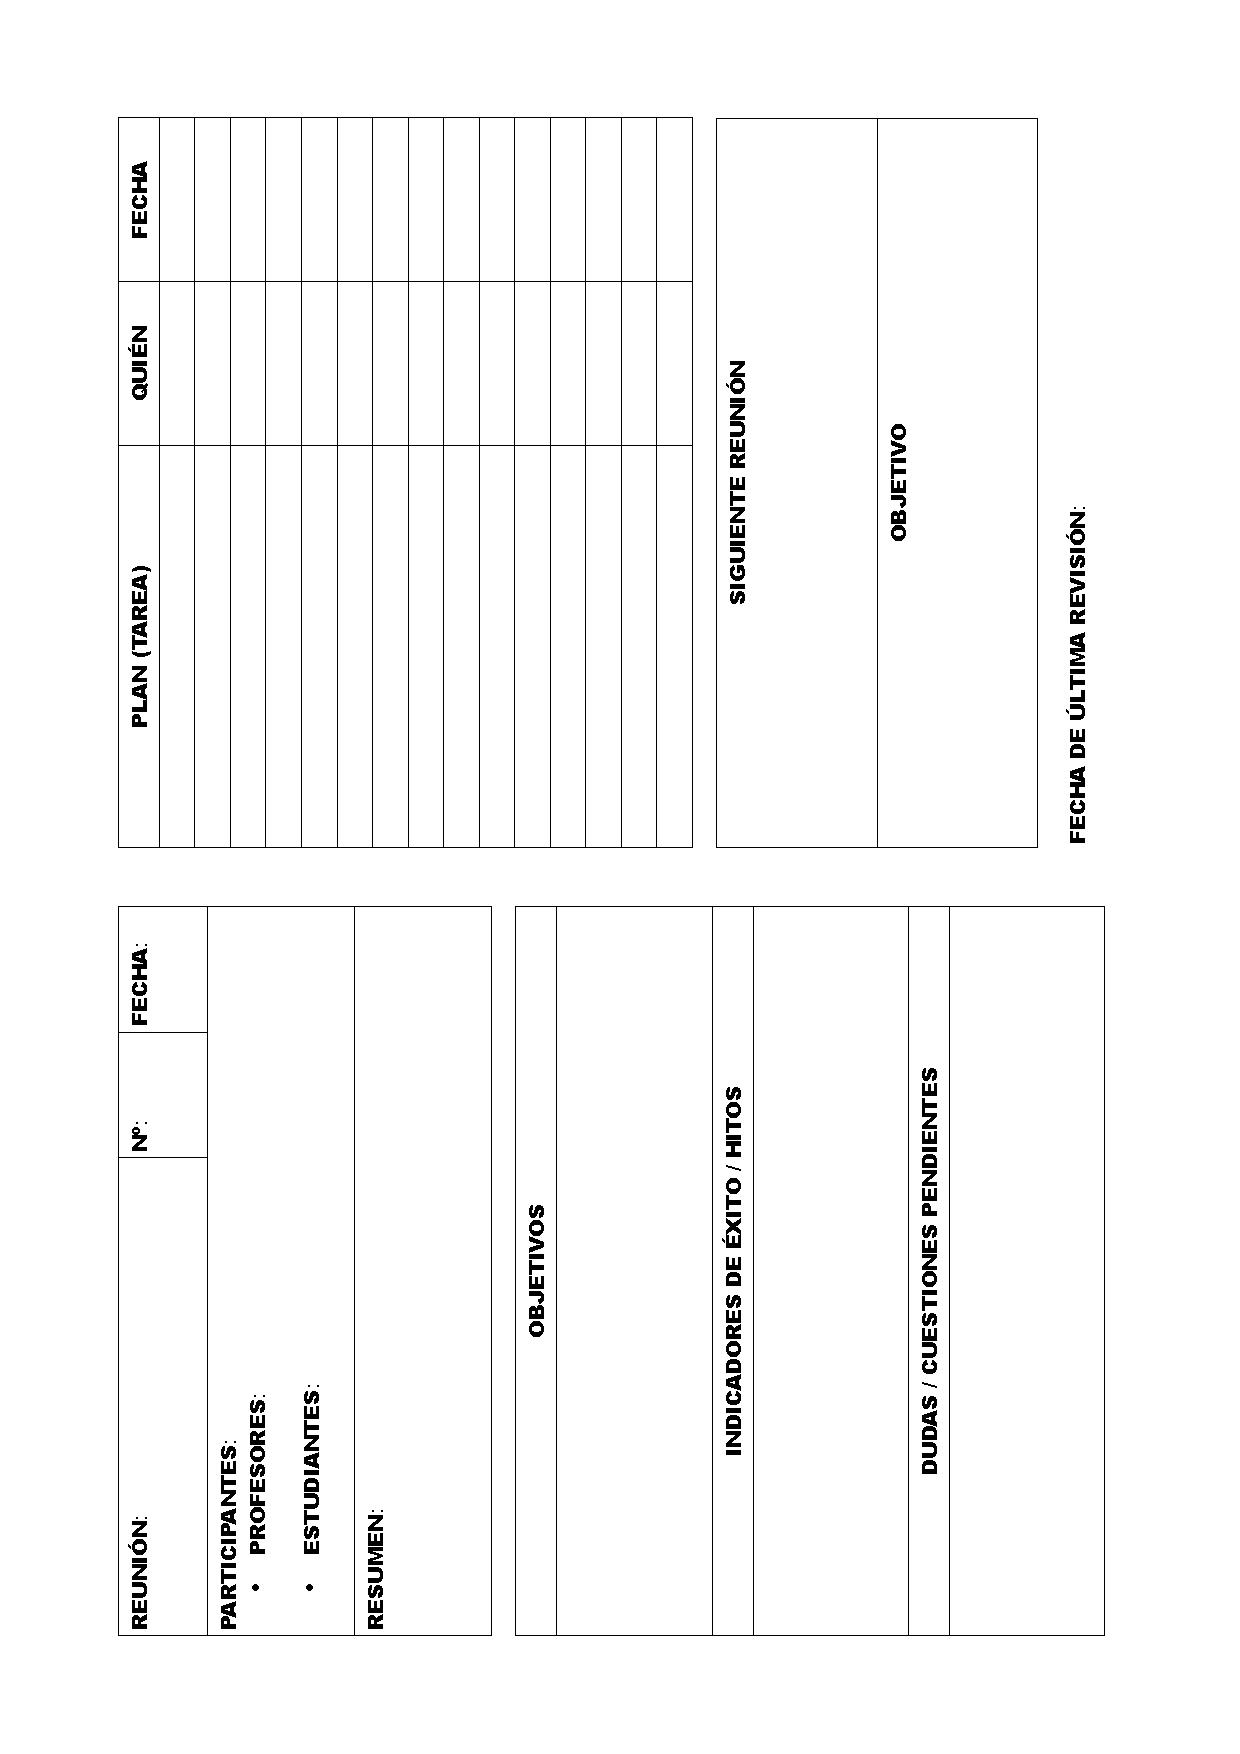
\includepdf[pages=1-]{meetings/template.pdf}

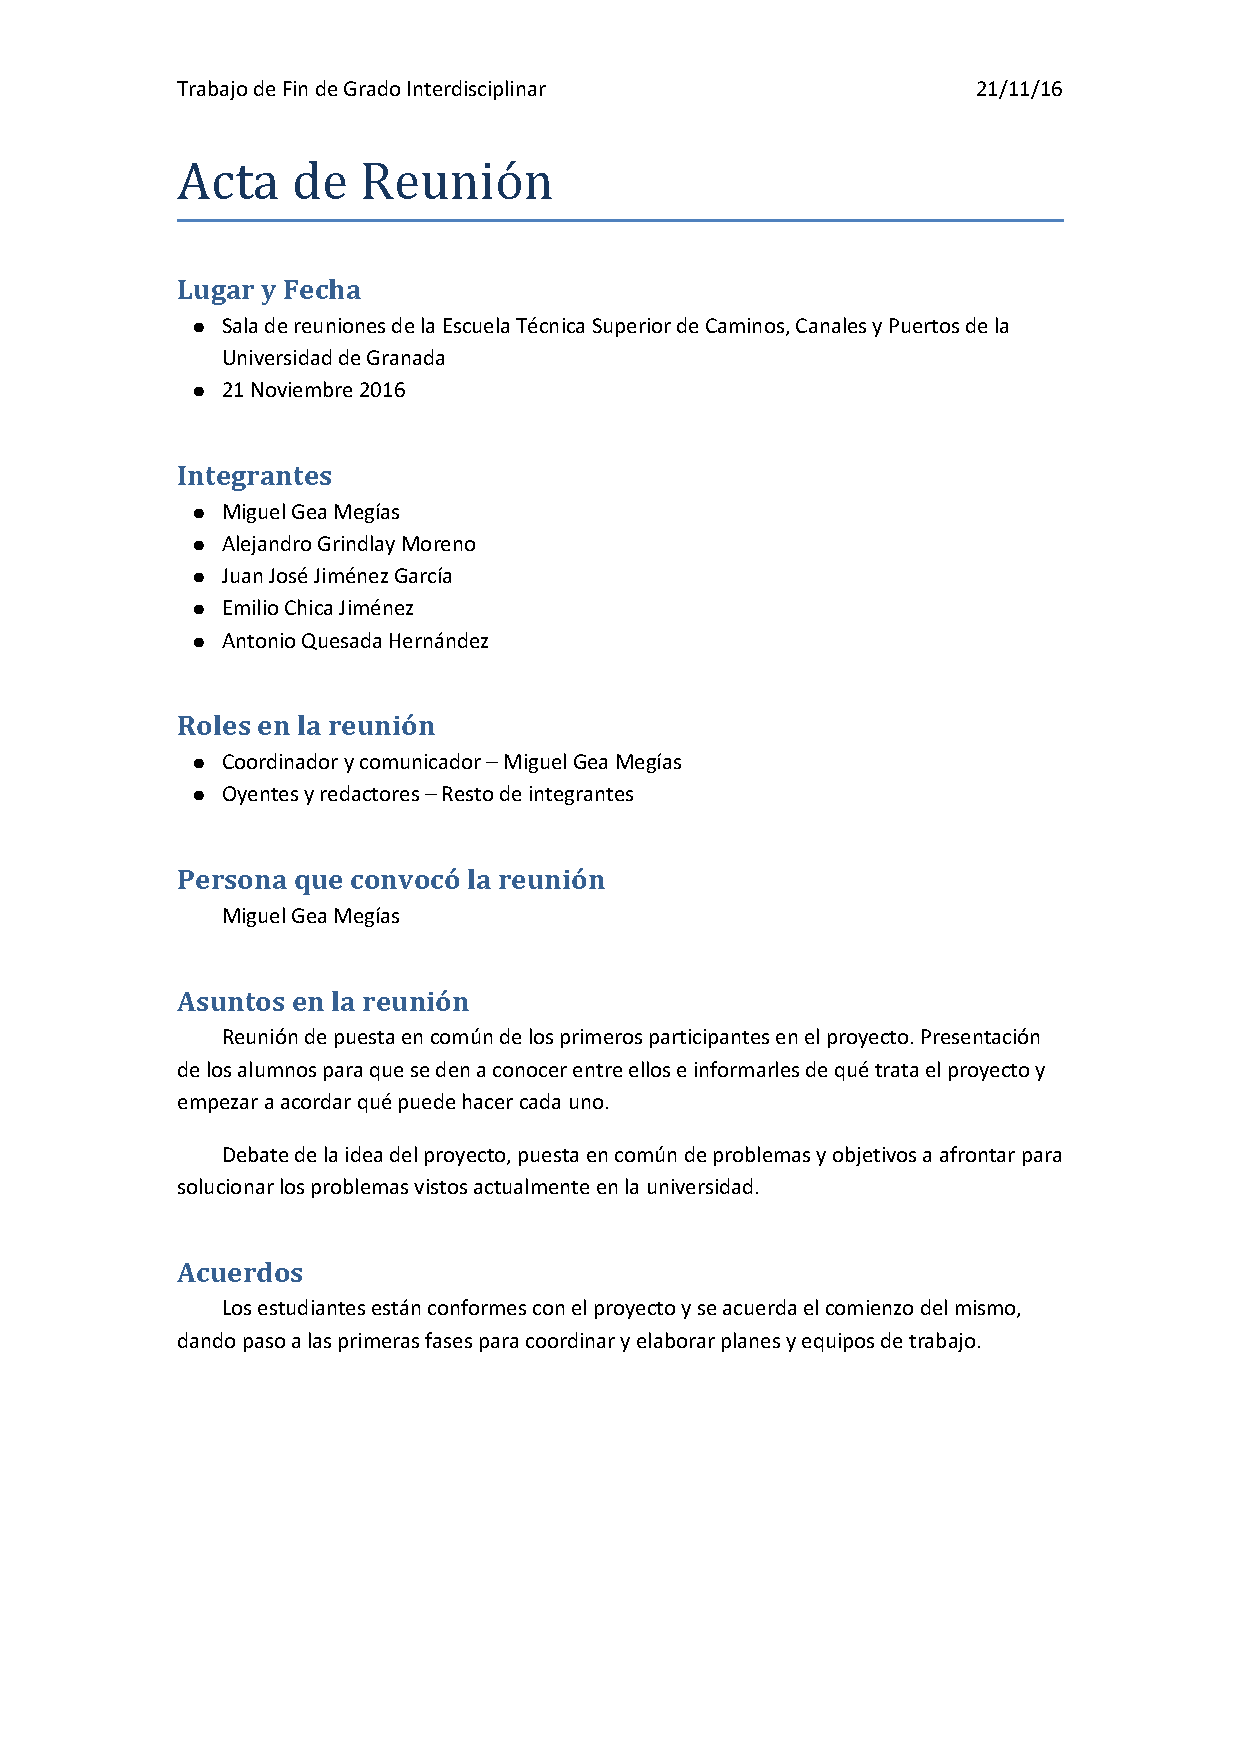
\includepdf[pages=1-]{meetings/01.pdf}
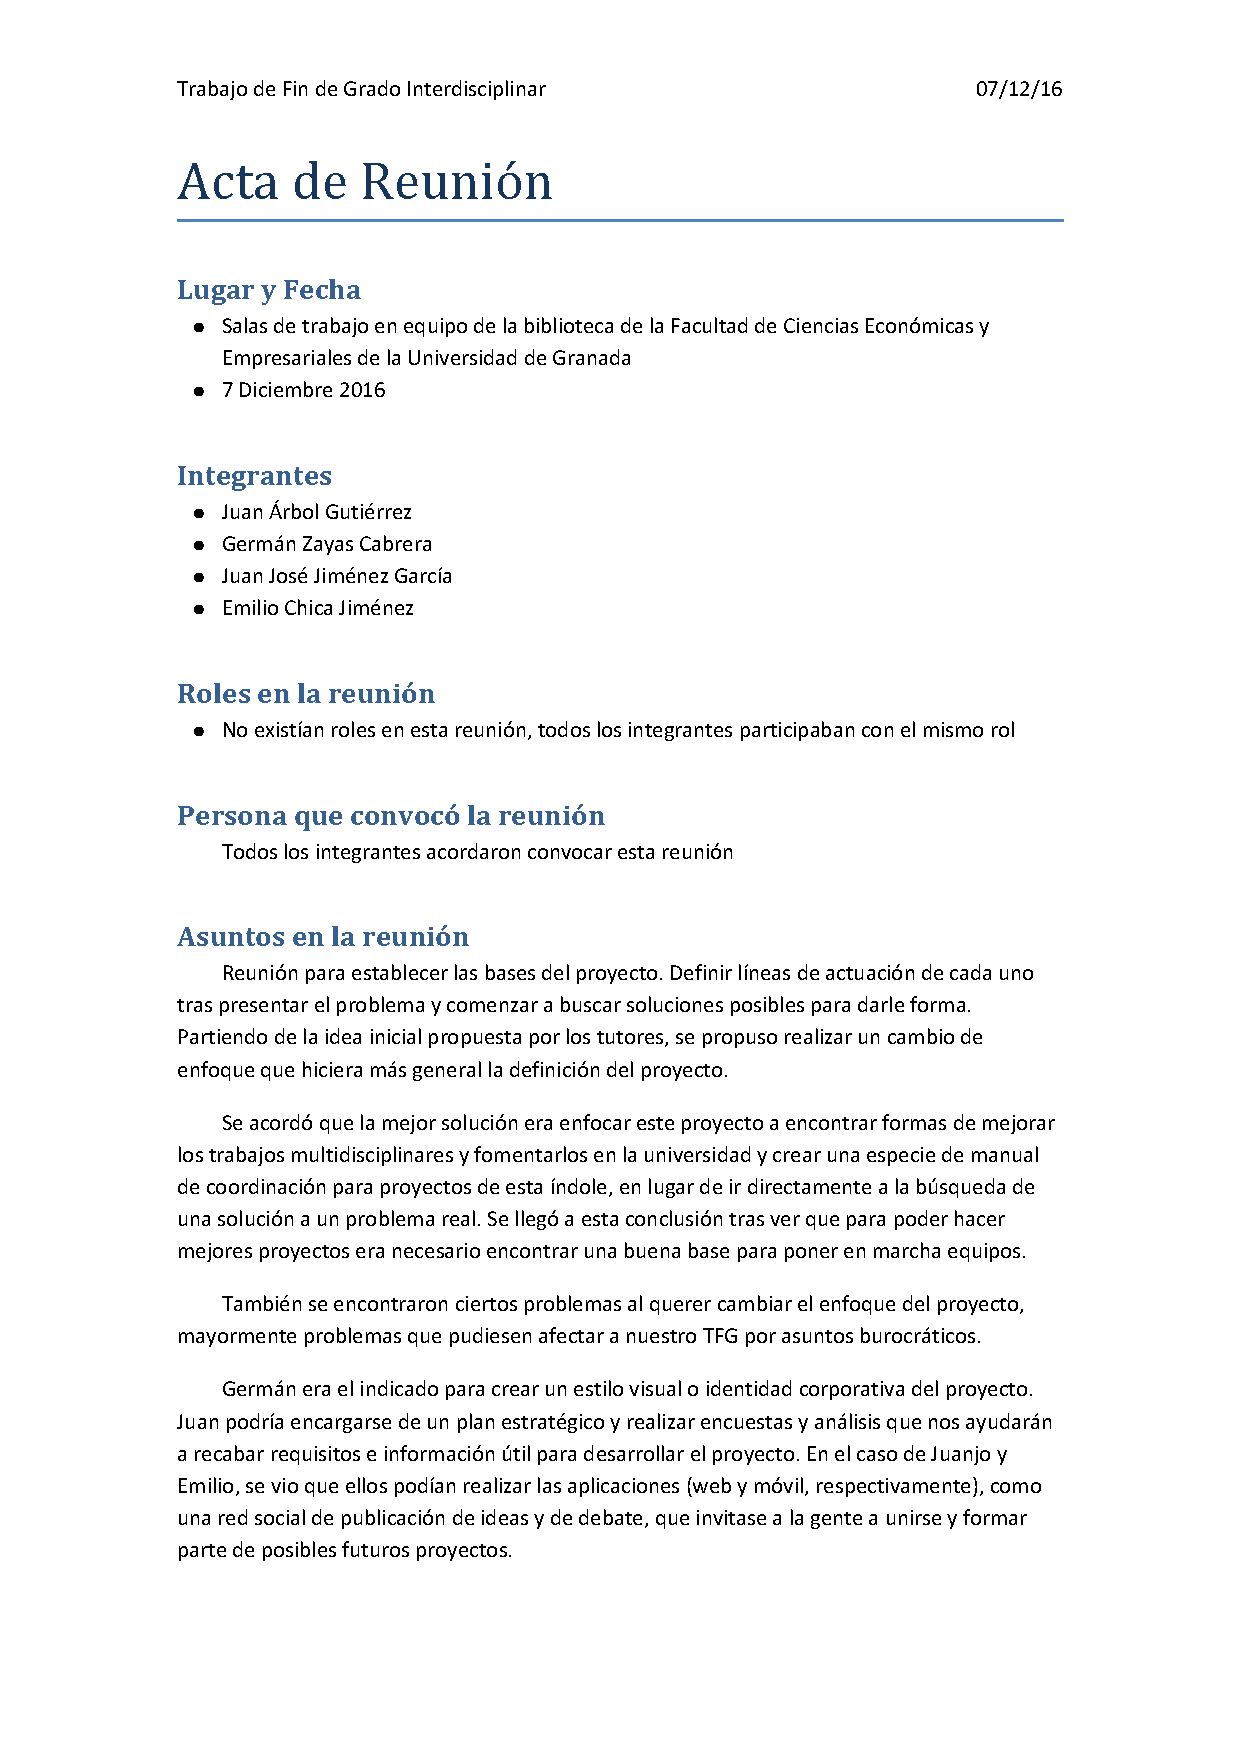
\includepdf[pages=1-]{meetings/02.pdf}
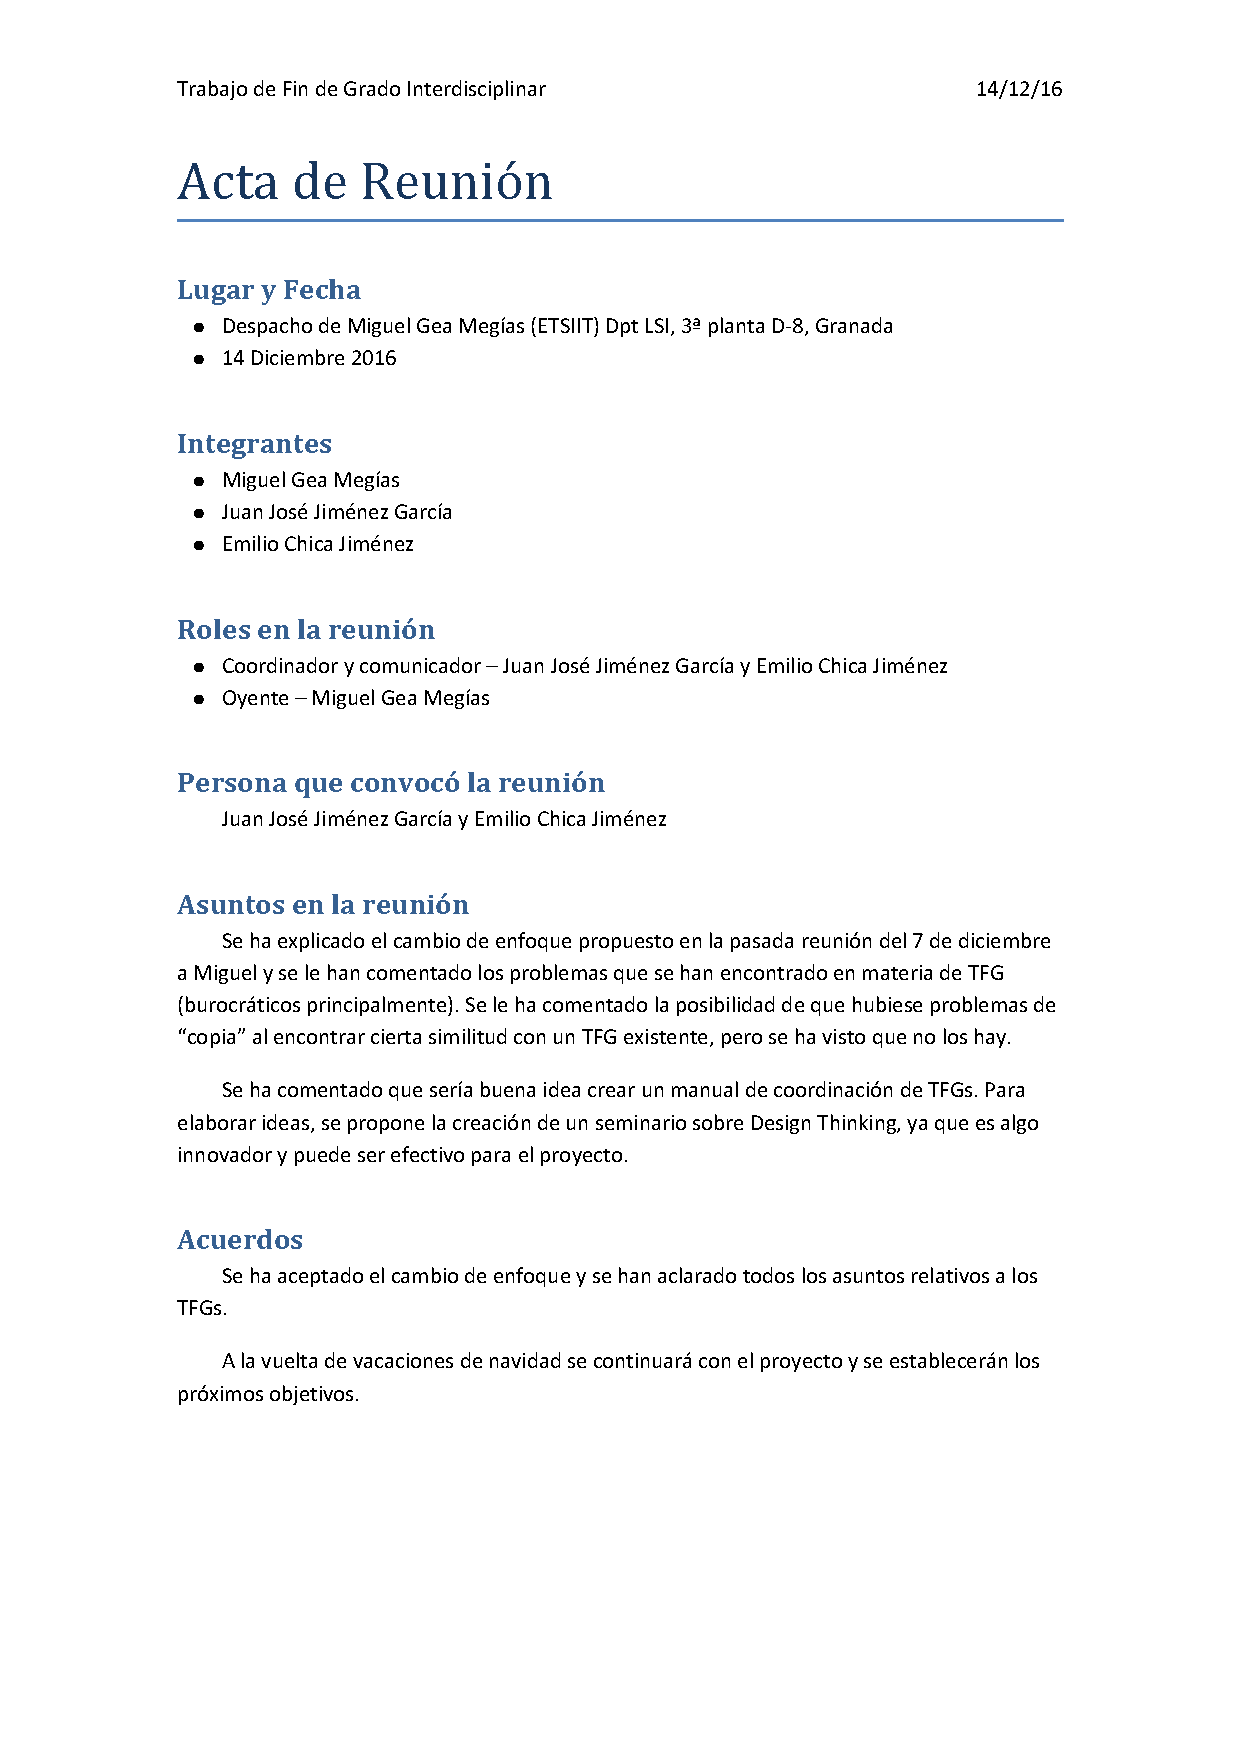
\includepdf[pages=1-]{meetings/03.pdf}
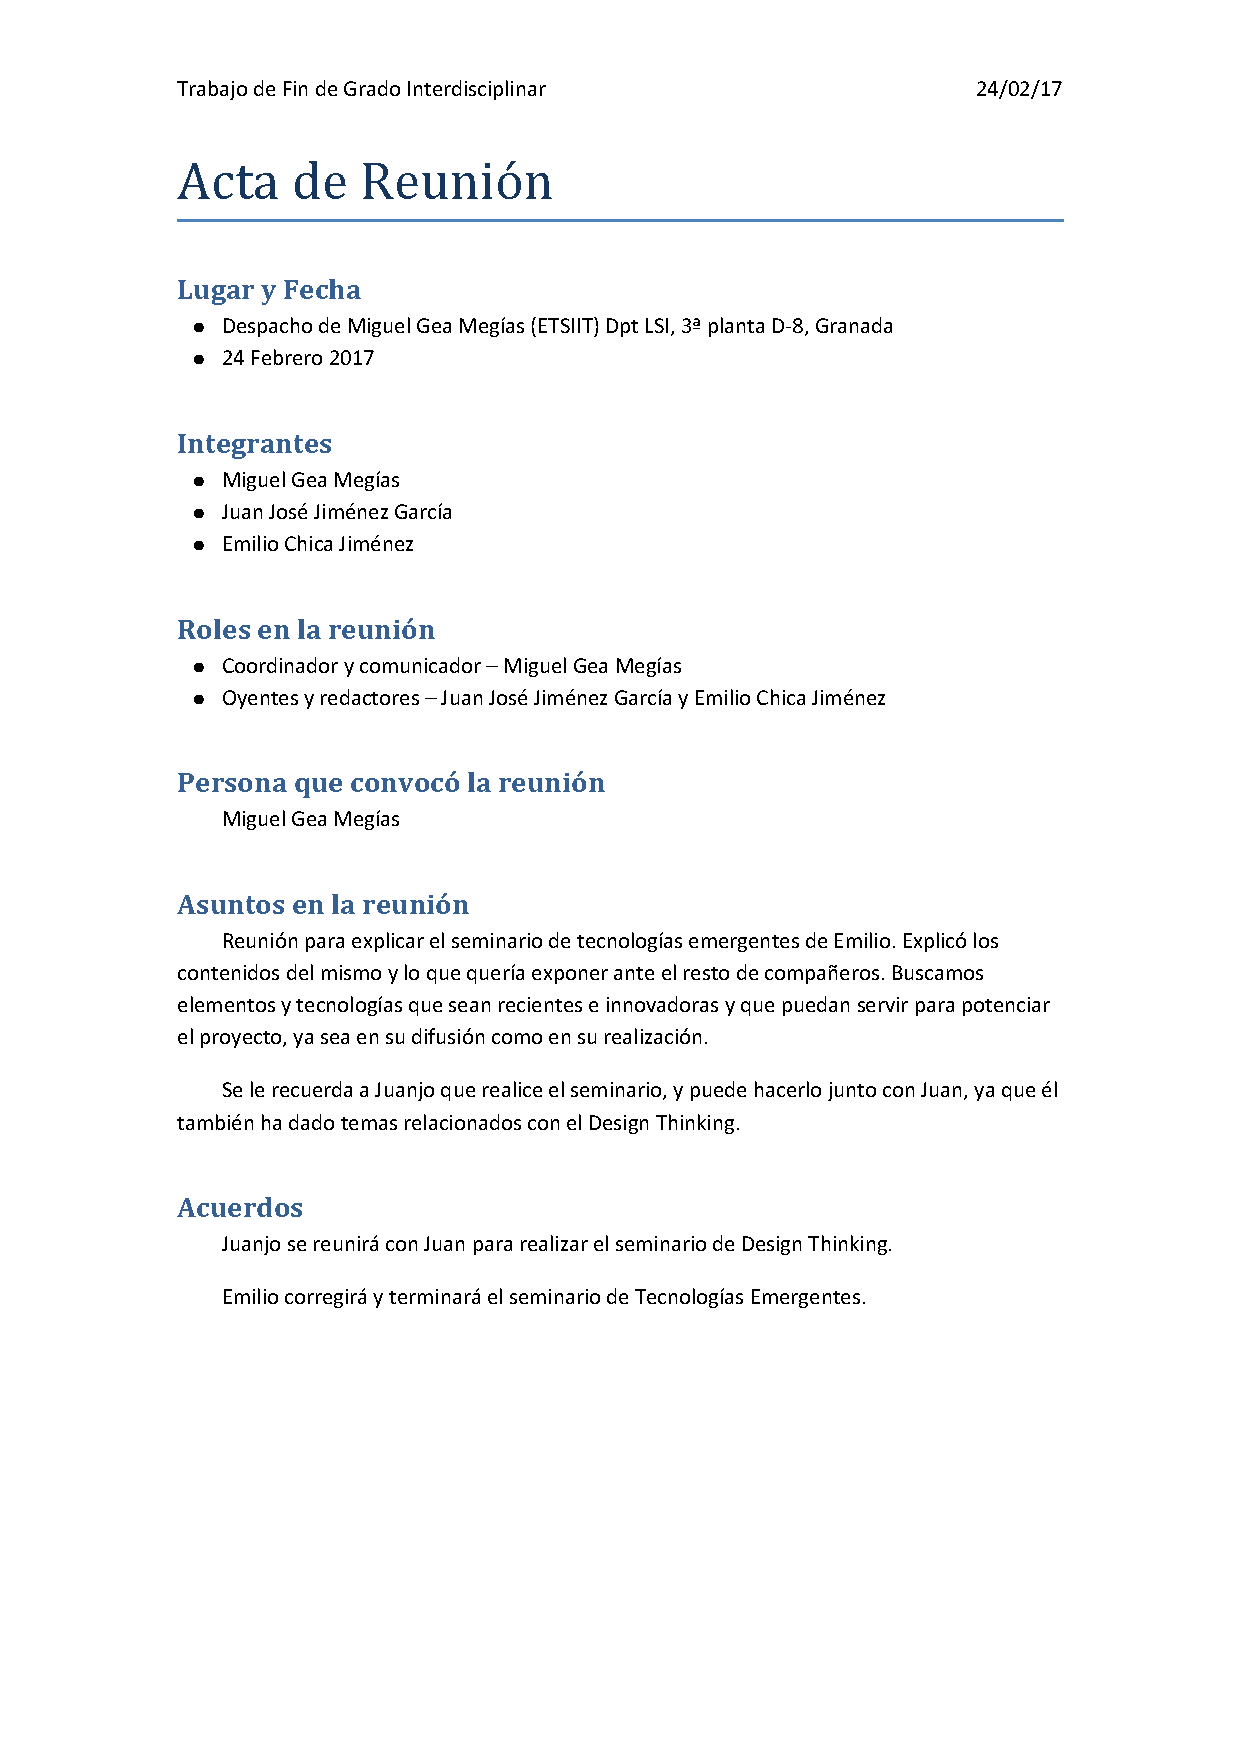
\includepdf[pages=1-]{meetings/04.pdf}
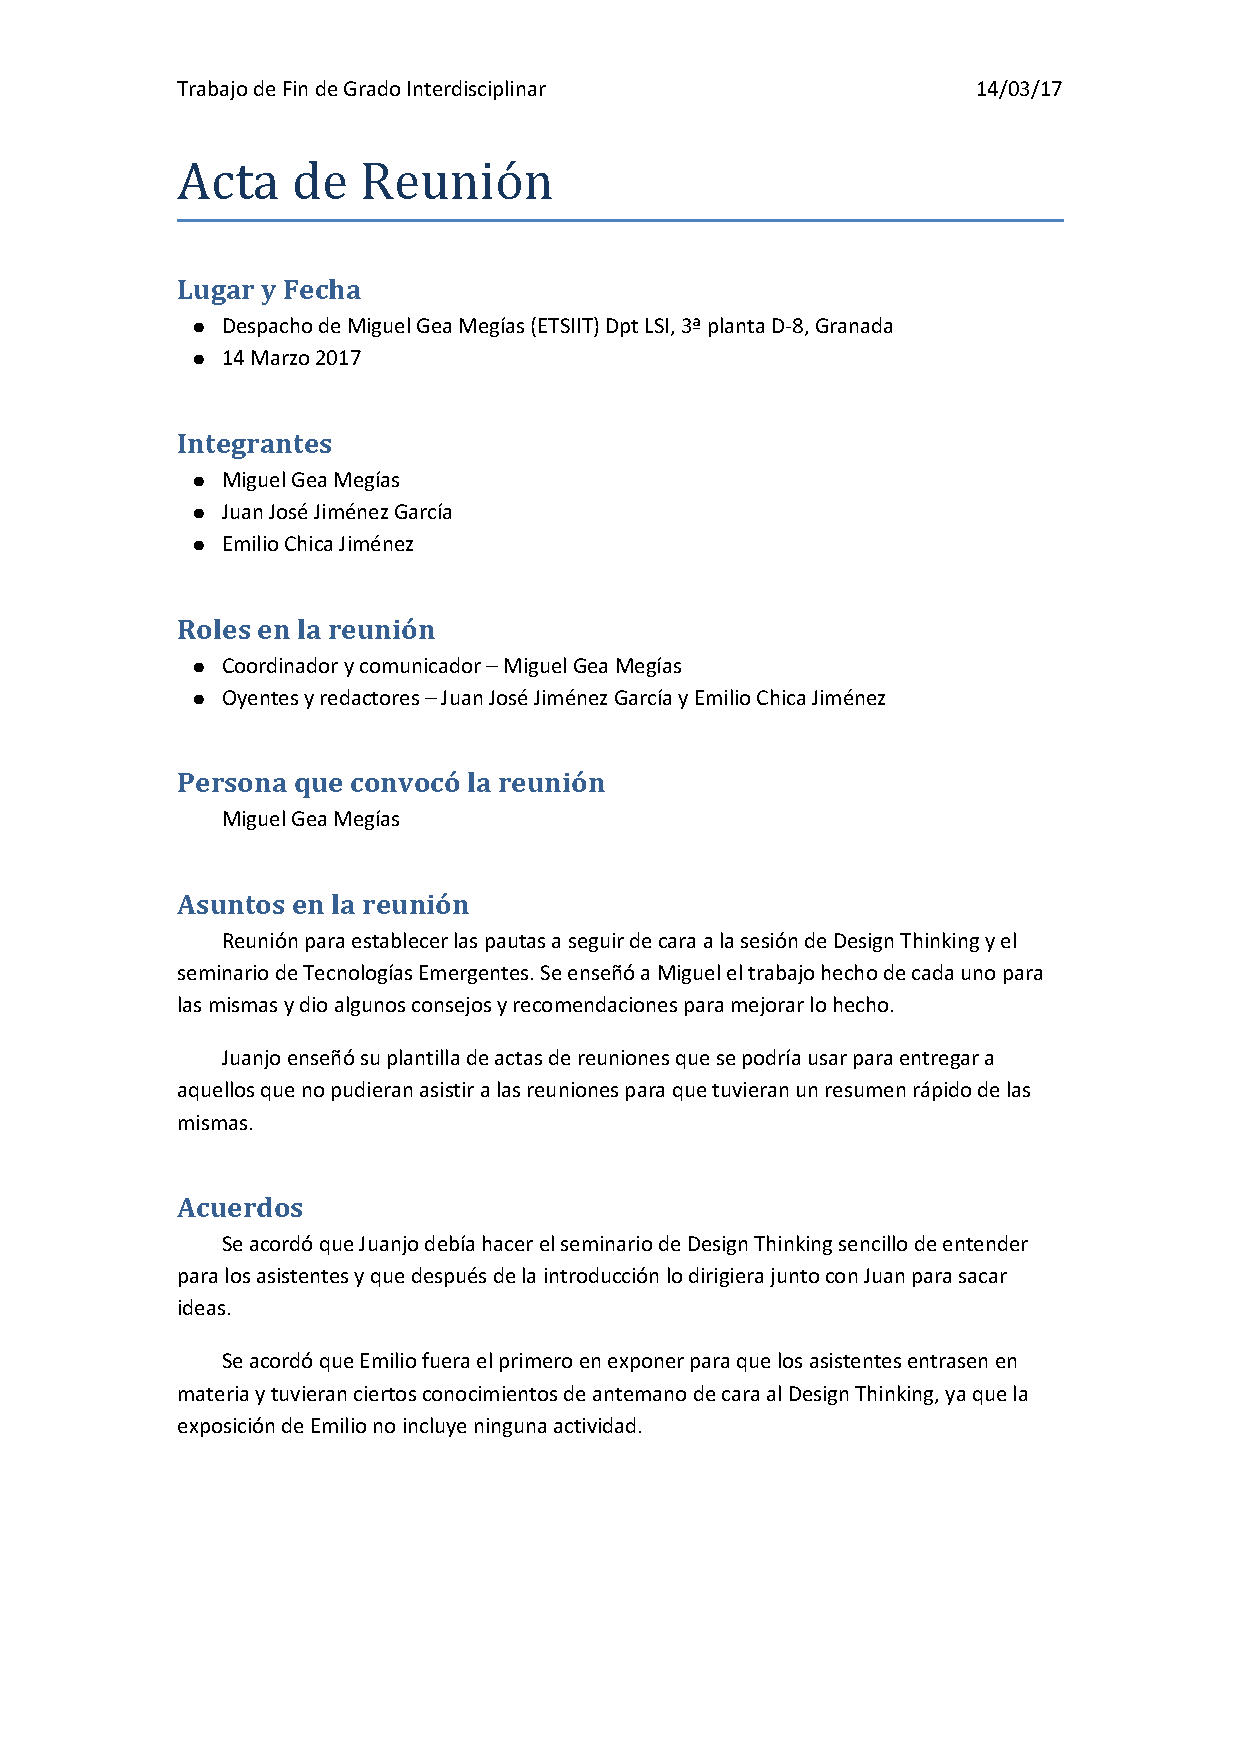
\includepdf[pages=1-]{meetings/05.pdf}
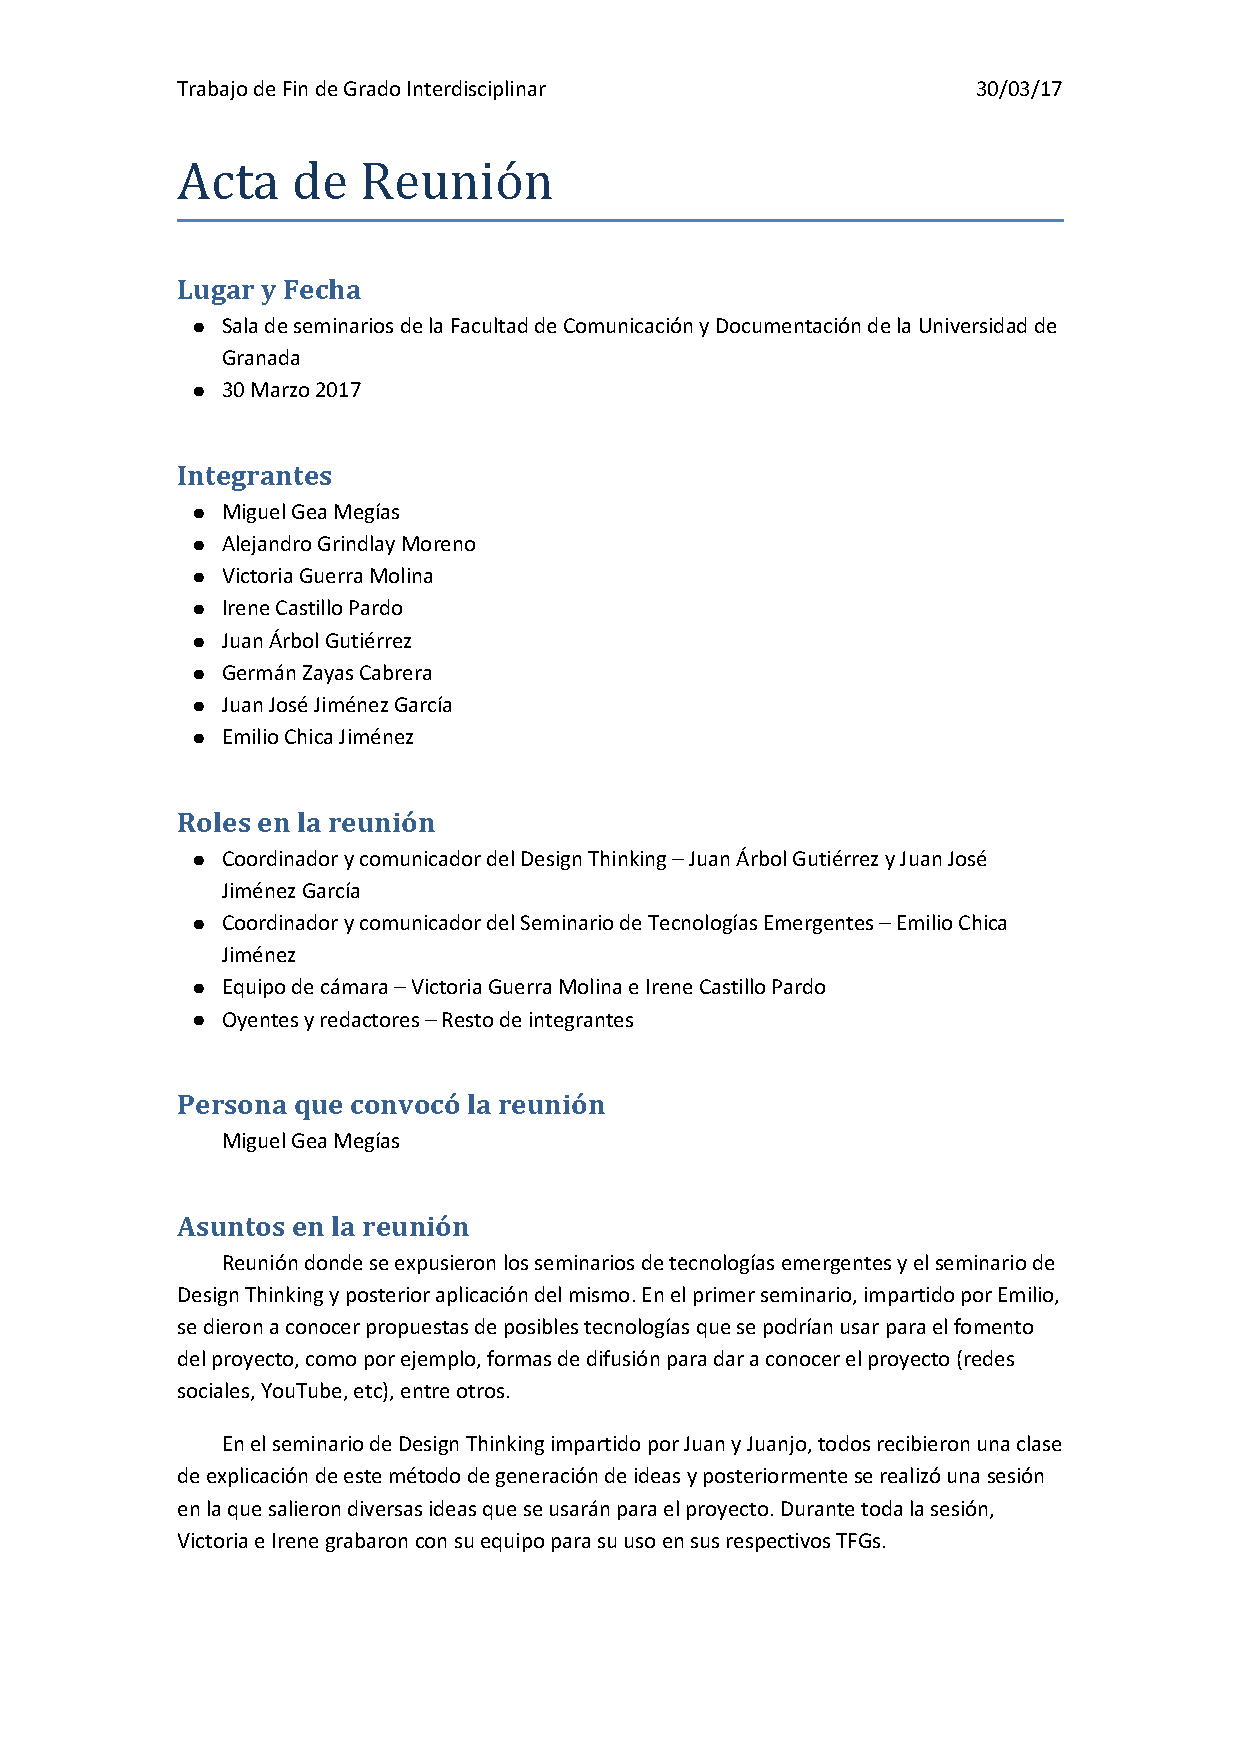
\includepdf[pages=1-]{meetings/06.pdf}
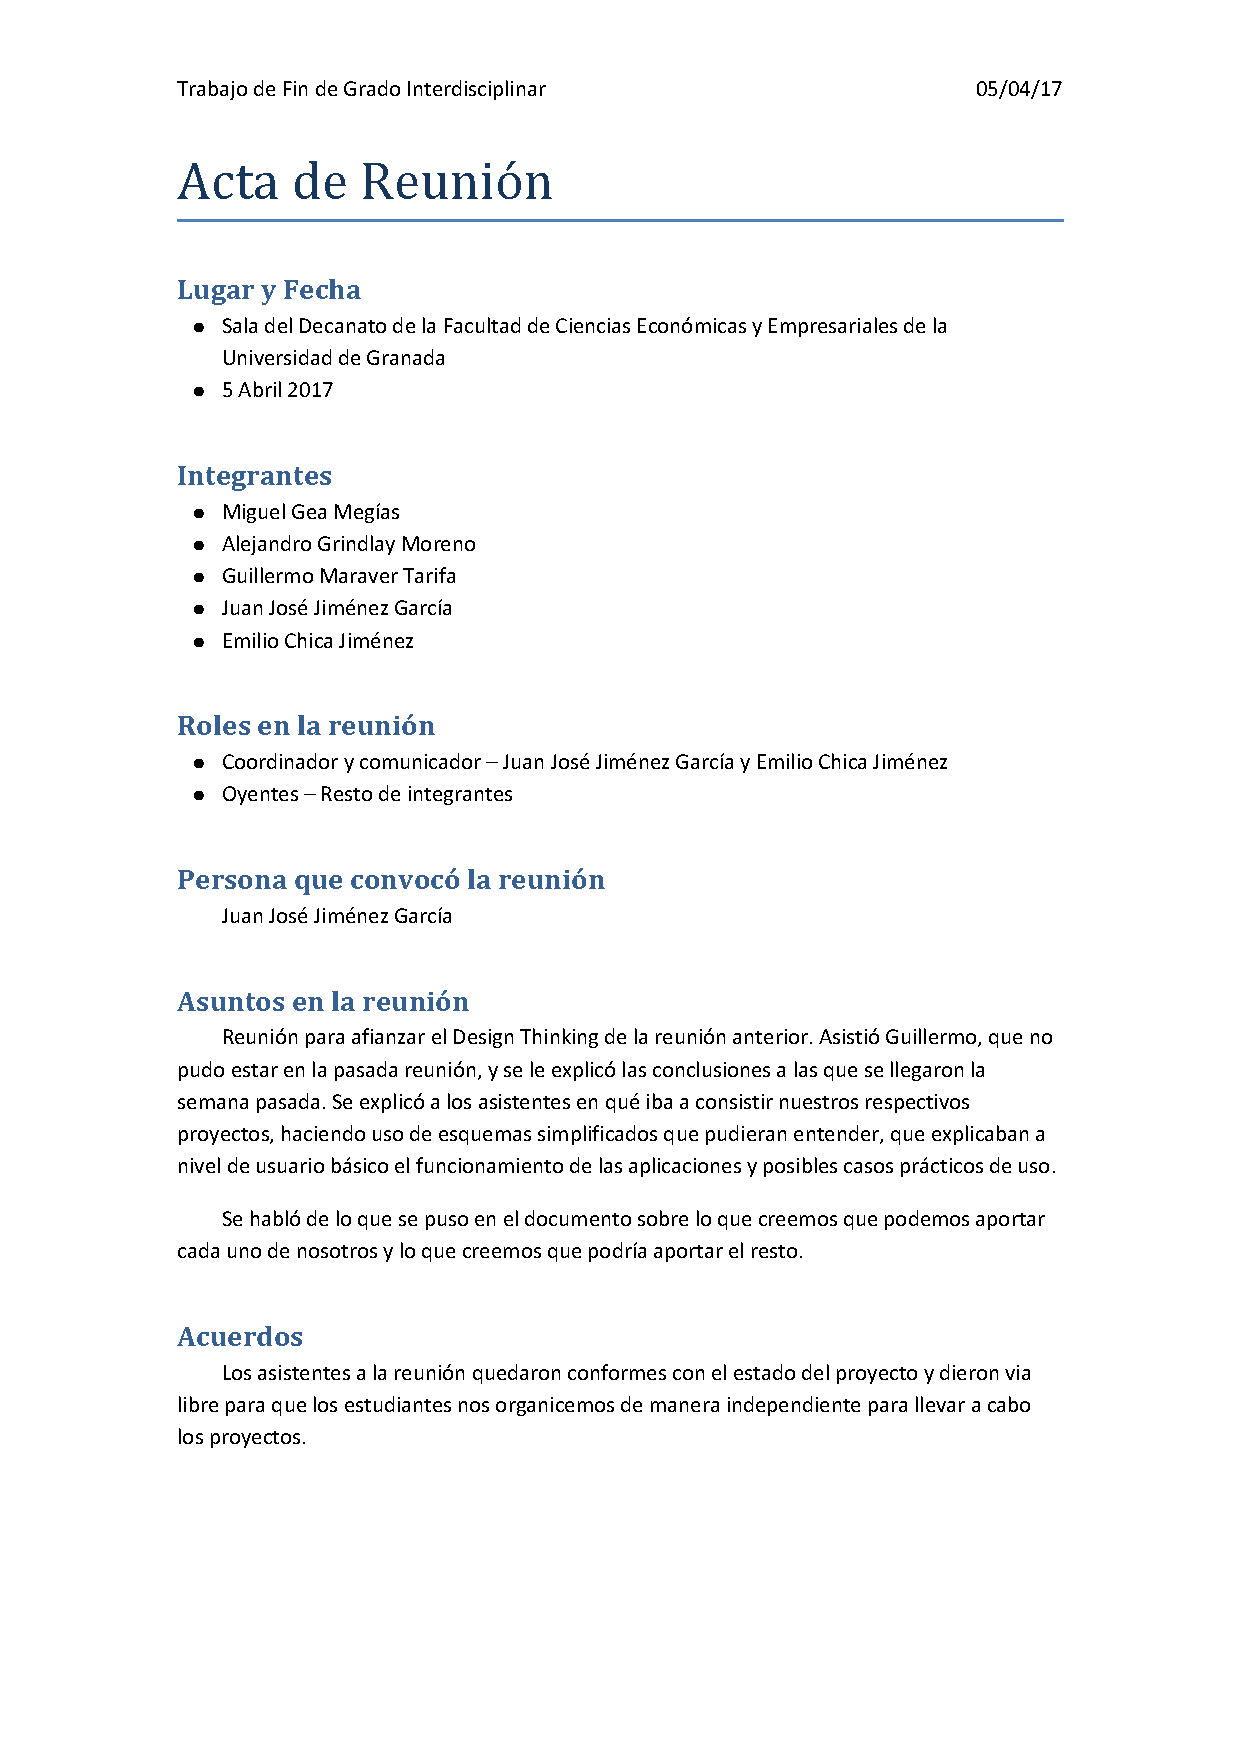
\includepdf[pages=1-]{meetings/07.pdf}
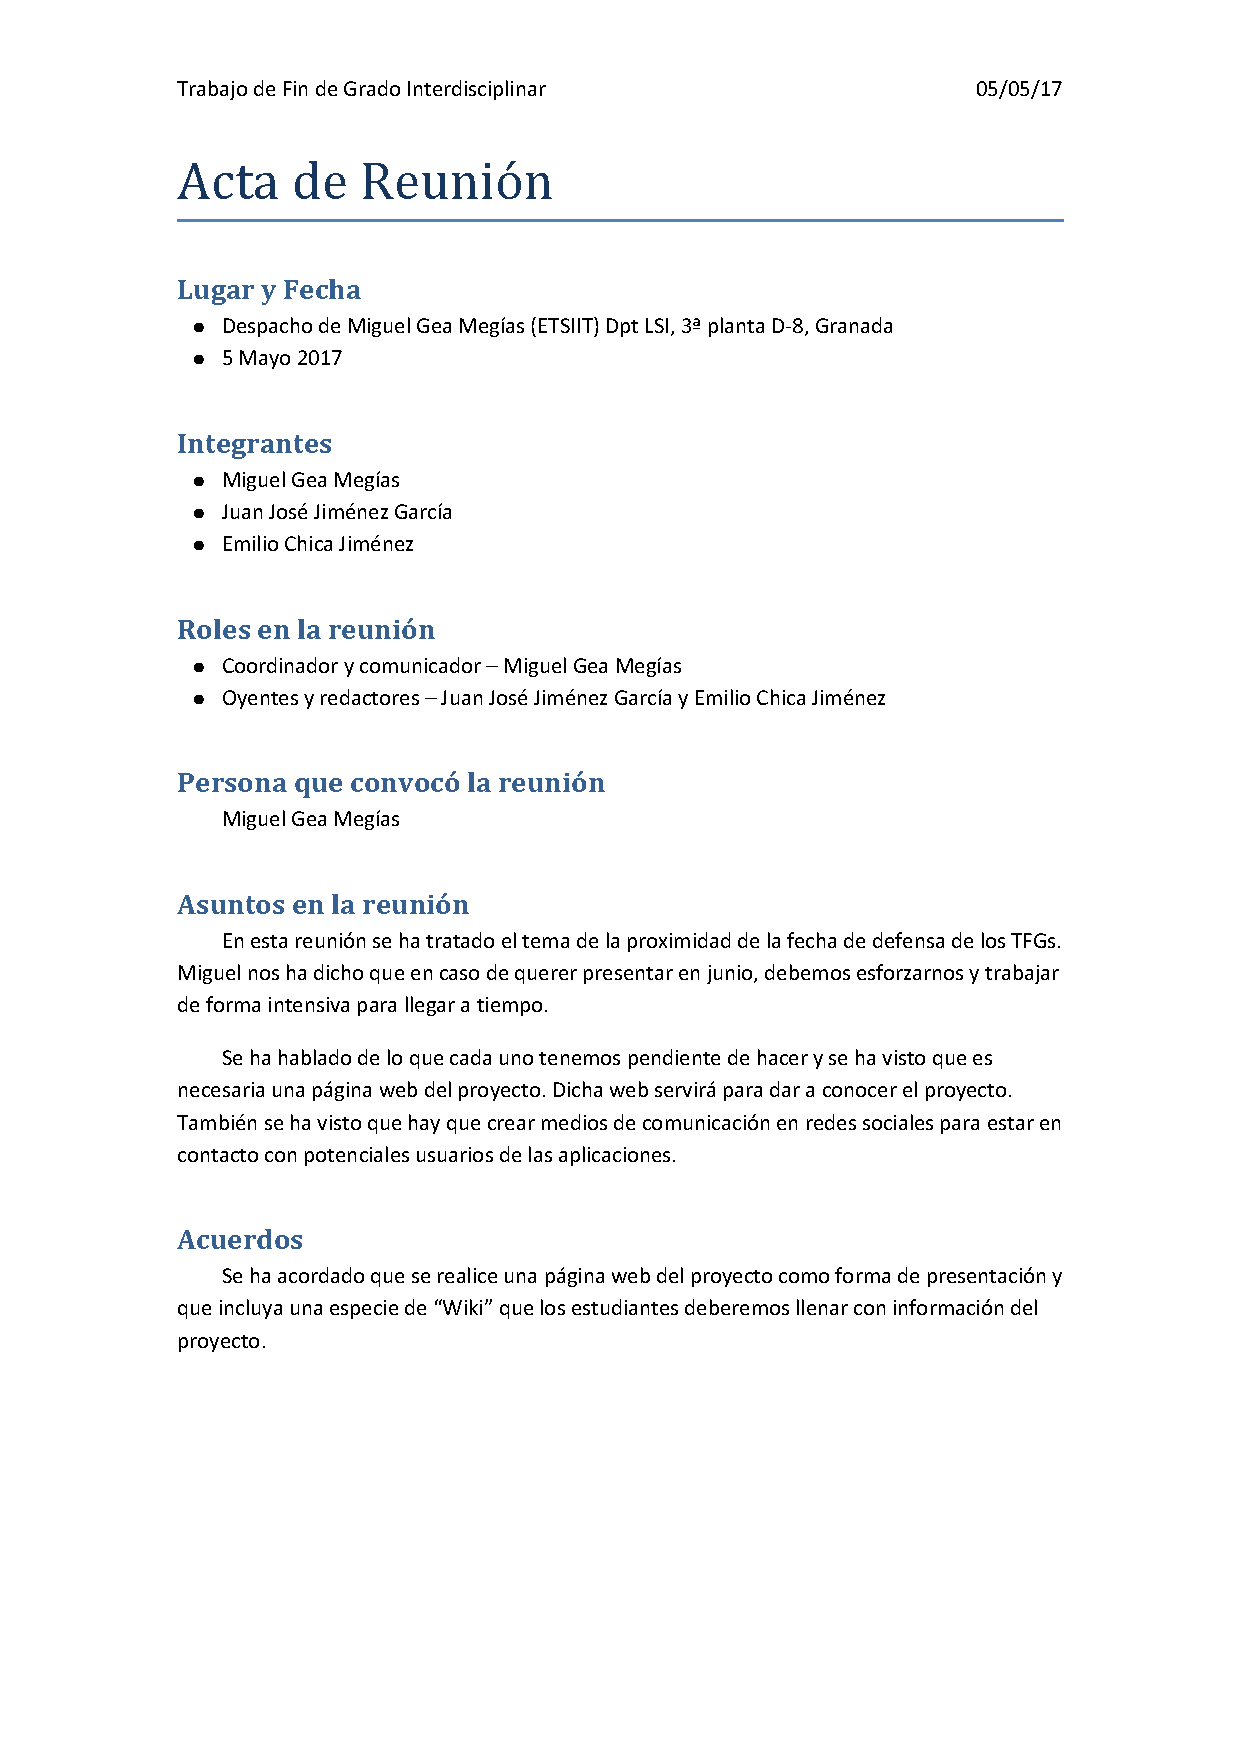
\includepdf[pages=1-]{meetings/08.pdf}
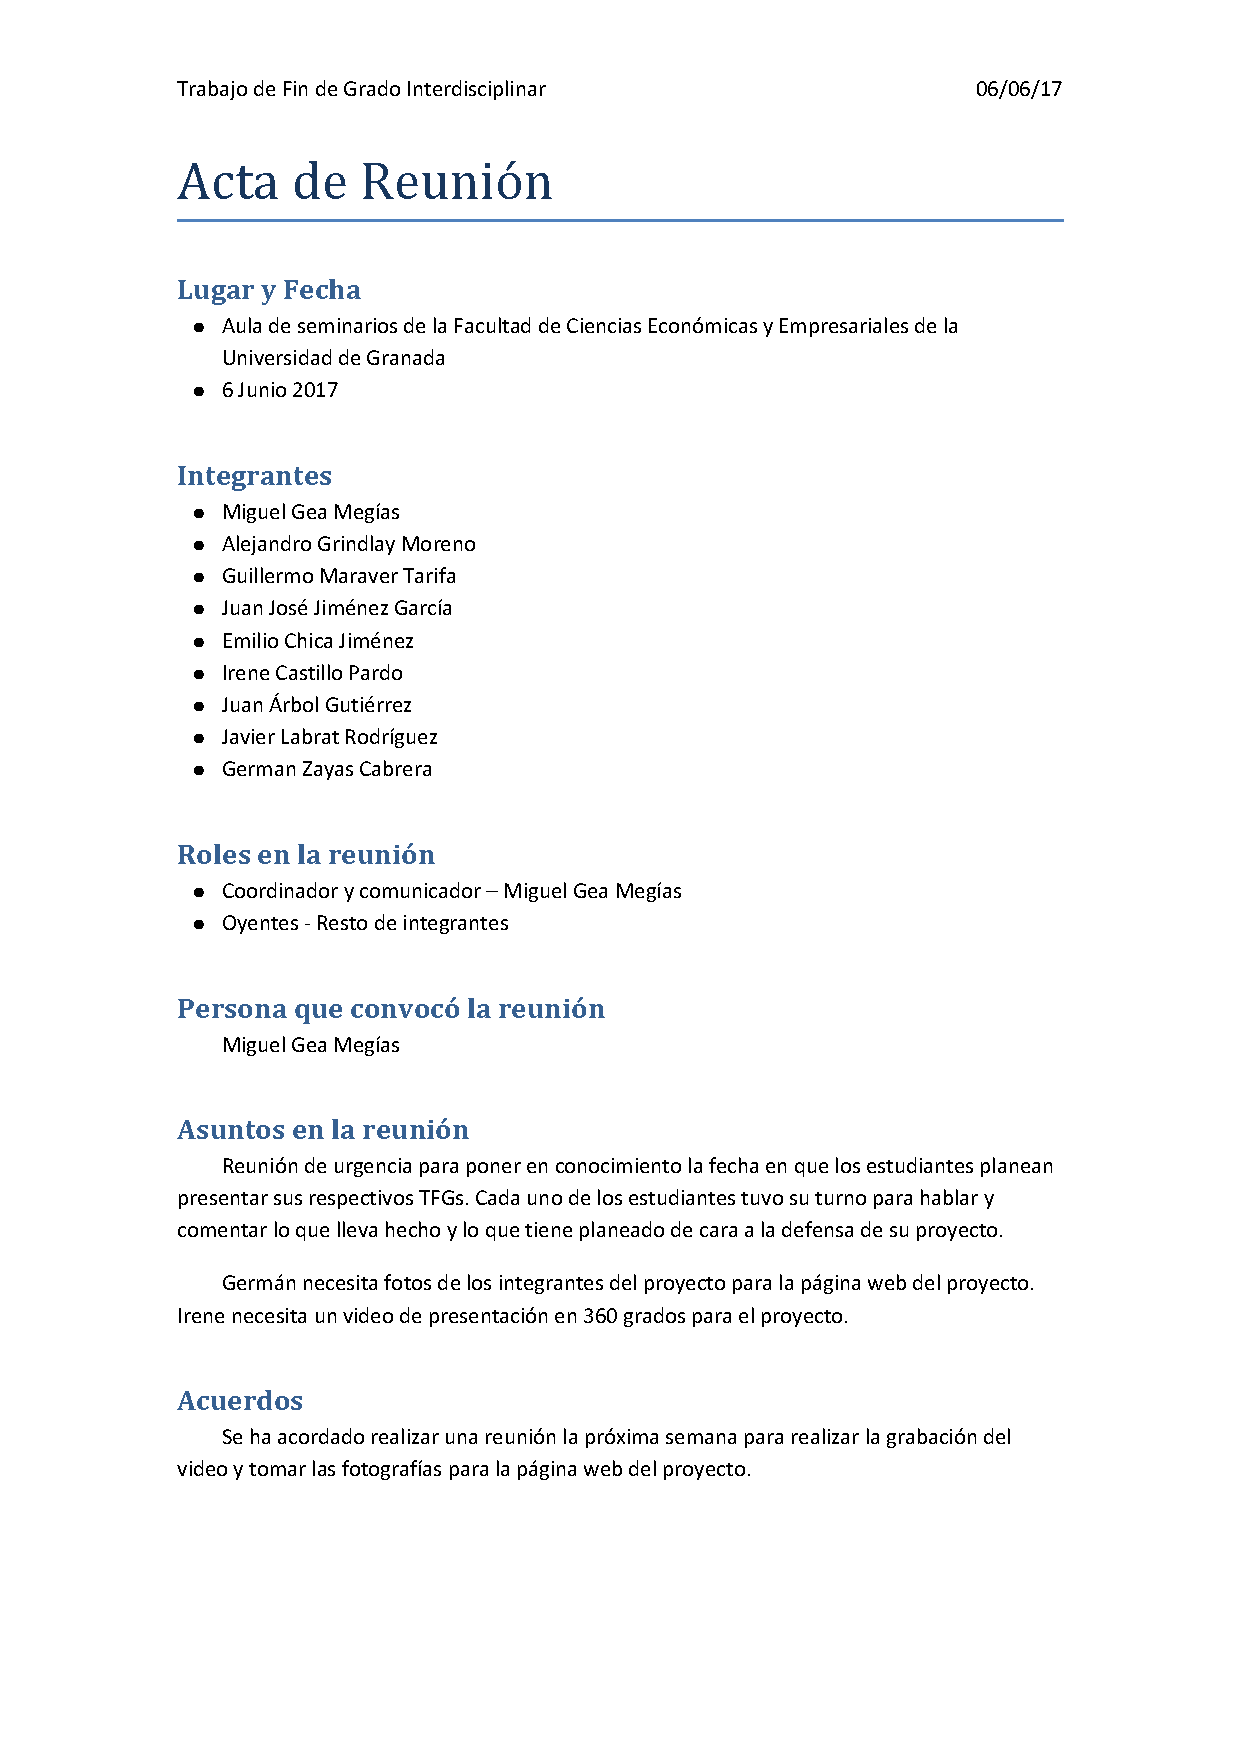
\includepdf[pages=1-]{meetings/09.pdf}
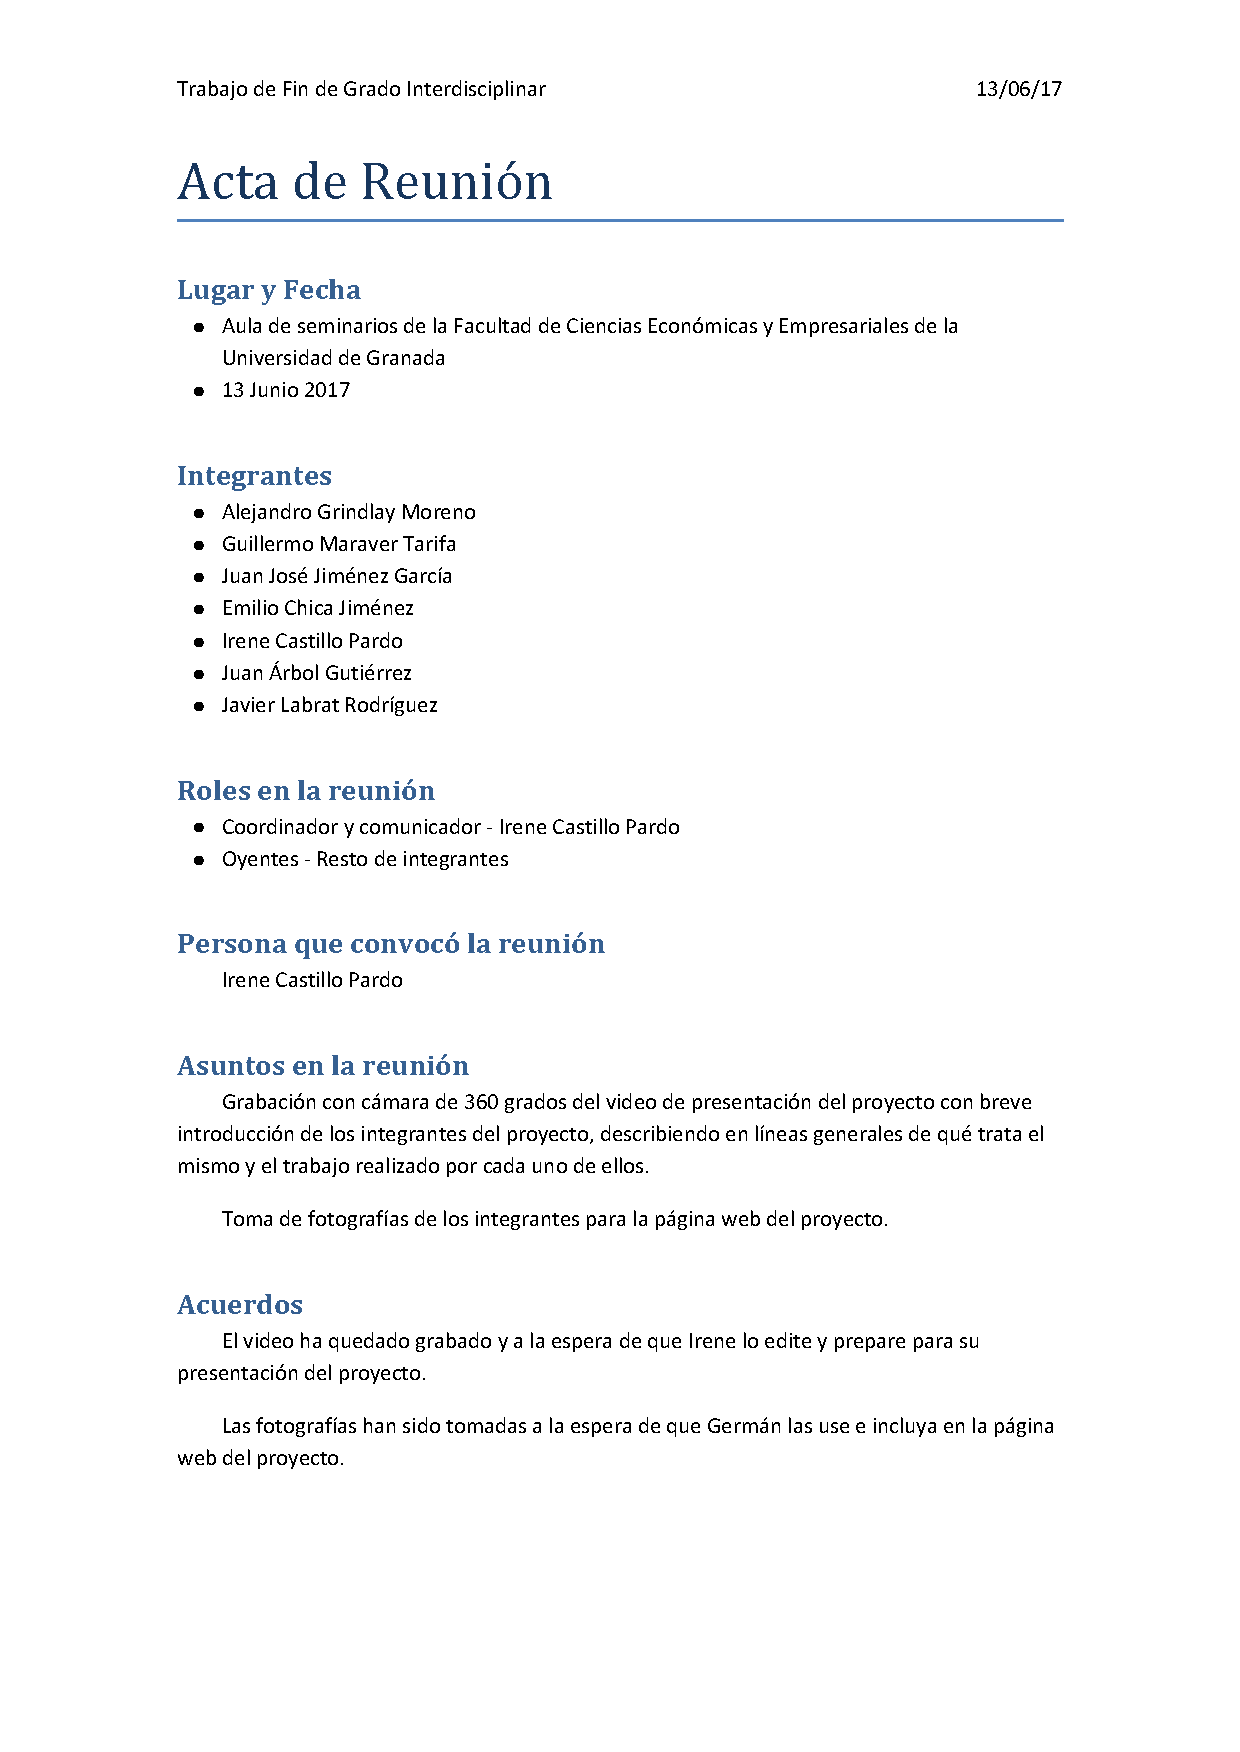
\includepdf[pages=1-]{meetings/10.pdf}


% Glosario de términos
\backmatter
\begingroup
	\setlength\parindent{0pt}
	\chapter{Glosario de términos}

\begin{description}
  
\end{description}

\endgroup

% Bibliografía
\newpage
\begin{thebibliography}{99}
	\addcontentsline{toc}{chapter}{Bibliografía}

\subsection*{Páginas web consultadas durante la realización del proyecto}

\bibitem{globalizacion} {\tt Globalización - Wikipedia}\\
\url{https://es.wikipedia.org/wiki/Globalizaci%C3%B3n}

\bibitem{globalreport} {\tt Globalization Report 2016 - Who benefits most from globalization?}\\
\url{https://www.bertelsmann-stiftung.de/fileadmin/files/BSt/Publikationen/GrauePublikationen/NW_Globalization_Report_2016.pdf}

\bibitem{internetusage} {\tt Wikipedia - Global Internet usage stats from the International Telecommunications Union}\\
\url{https://en.wikipedia.org/wiki/Global_Internet_usage#Internet_users}

\bibitem{ugremprende} {\tt UGR Emprendedora - Página principal}\\
\url{https://ugremprendedora.ugr.es/}

\bibitem{h2020} {\tt Horizon 2020 - Página principal}\\
\url{https://ec.europa.eu/programmes/horizon2020/}

\bibitem{agilereport} {\tt Top 10 Insights from the 11th Annual State of Agile Report}\\
\url{https://explore.versionone.com/state-of-agile/top-10-insights-from-the-11th-annual-state-of-agile-report-2}

\bibitem{health1} {\tt PubMed Central - Multidisciplinary in-hospital teams improve patient outcomes: A review}\\
\url{https://www.ncbi.nlm.nih.gov/pmc/articles/PMC4173201/}

\bibitem{health2} {\tt PubMed Central - Benefits of multidisciplinary teamwork in the management of breast cancer}\\
\url{https://www.ncbi.nlm.nih.gov/pmc/articles/PMC3929250/}

\bibitem{neuroped} {\tt Imagen original de NeuroPed - Enlace}\\
\url{http://www.neuroped.es/equipo-multidisciplinar/}

\bibitem{medialabugr} {\tt Medialab UGR - Página principal}\\
\url{http://medialab.ugr.es/}

\bibitem{linkuma} {\tt Link by UMA-ATech (Universidad de Málaga) - Página principal}\\
\url{http://www.link.uma.es/}

\bibitem{linkimage} {\tt Fotografía original de Geek and Tech Girls}\\
\url{https://geekandtechgirls.github.io/We-Create-Technology/}

\bibitem{linkedin} {\tt LinkedIn - Página principal}\\
\url{https://es.linkedin.com/}

\bibitem{kickstarter} {\tt Kickstarter - Página principal}\\
\url{https://www.kickstarter.com/}

\bibitem{responsivelink} {\tt Página de inicio de \textit{Responsive Web Design}}\\
\url{https://responsivedesign.is/}

\bibitem{contentwater} {\tt Imagen original de Wikimedia - Enlace}\\
\url{https://commons.wikimedia.org/wiki/File:Content_is_like_water.png}

\bibitem{framework} {\tt Framework - Wikipedia}\\
\url{https://es.wikipedia.org/wiki/Framework}

\bibitem{startup} {\tt Startup - Wikipedia}\\
\url{https://es.wikipedia.org/wiki/Empresa_emergente}

\bibitem{designthinkinglink} {\tt Design Thinking en Español - Página oficial}\\
\url{http://designthinking.es/inicio/index.php}

\subsection*{Libros consultados}

\bibitem{gangoffour}
Gamma, E., Helm, R., Johnson, R. and Vlissides, J. 1994. {\em Design Patterns. Elements of Reusable Object-Oriented Software}. Addison Wesley.

\bibitem{brandon}
M. Brandon, D. 2008. {\em Software Engineering for Modern Web Applications: Methodologies and Technologies}. Information Science Reference.

\bibitem{pressman}
Pressman, R. 1982. {\em Software Engineering - A Practitioner's Approach}. McGraw-Hill Higher Education.

\bibitem{pressmanweb}
Pressman, R. and Lowe, D. 2009. {\em Web Engineering - A Practitioner's Approach}. McGraw-Hill Higher Education.

\bibitem{headfirstpatterns}
Sierra, K., Freeman, E., Robson, E. and Bates, B. 2004. {\em Head First Dessign Patterns. A Brain-Friendly Guide}. O'Reilly.

\subsection*{Páginas de principales productos y programas usados}

\bibitem{bootstrap} {\tt Bootstrap Framework - Página principal}\\
\url{https://getbootstrap.com/}

\bibitem{laravel} {\tt Laravel - Página principal}\\
\url{https://laravel.com}

\bibitem{xampp} {\tt XAMPP - Página oficial}\\
\url{https://www.apachefriends.org/es/index.html}

\bibitem{slack} {\tt Slack - Página oficial}\\
\url{https://slack.com/}

\bibitem{googlecalendar} {\tt Google Calendar - Página oficial}\\
\url{https://www.google.com/calendar}

\bibitem{googledrive} {\tt Google Drive - Página oficial}\\
\url{https://www.google.com/drive}

\bibitem{whatsapp} {\tt WhatsApp - Página oficial}\\
\url{https://www.whatsapp.com/}

\subsection*{Otros recursos utilizados}

\bibitem{laraveldocs} {\tt Documentación oficial de Laravel 5.5}\\
\url{https://laravel.com/docs/5.5/}

\bibitem{bootstrapdocs} {\tt Documentación oficial de Bootstrap 3.3}\\
\url{https://getbootstrap.com/docs/3.3/}\\

Apuntes de asignaturas del \textbf{Grado en Ingeniería Informática}, tales como:
\begin{itemize}
    \item Desarrollo de Aplicaciones para Internet
    \item Sistemas de Información Basados en Web
    \item Desarrollo de Software
    \item Fundamentos de Ingeniería del Software
    \item Dirección y Gestión de proyectos
    \item Metodologías de Desarrollo Ágil
    \item Diseño y Desarrollo de Sistemas de Información
\end{itemize}

\end{thebibliography}

\chapter*{}
\thispagestyle{empty}

\end{document}
